% basically this is a template file, you should be able to take it and
% start running.

% the philosophy behind this template is that each chapter or
% chapterlike section goes in a separate file and you use the \include
% command to input it into the final document.  The \includeonly
% command can be used so you only need to work on one or two chapters at a
% time (instead of having to either latex the entire book each time or
% losing cross-references and page numbering)

% copy this file and call it something like mythesis.tex

\documentclass[12pt]{report}
% note that the documentclass can take other option such as
% twoside - for double sided printing
% openright - if double side  chapters always start on odd pages
% openany - if double side chapters start on the next page even or odd
% 12pt can be replaced by 11pt

\usepackage{suthesis-2e}

%% load other packages you need
\input defs
\usepackage{suthesis-2e,graphicx,subfigure,setspace, topcapt,amssymb,amsmath}
%\usepackage{site} %did not work with hyperref
\usepackage{natbib} %works with hyperref
\usepackage[pdftex,bookmarks=true, colorlinks=true,linkcolor=blue,
pdfpagemode=UseOutlines, citecolor=blue, backref=page,
linktocpage=true ]{hyperref}
\usepackage[all]{hypcap} %to link to top of figure, not to top of caption
\bibpunct{[}{]}{,}{n}{,}{,} %settings for natbib



%% uncomment the following and create mythesis-macros.sty for all your
%% own macros.  This keeps this top level file looking fairly neat.
% \usepackage{mythesis-macros}

%% certain types of theses require special title page format.  See the
%% style file for the full list.  An example would be that for some of
%% the language departments. 
% \dualthesis \dept{Asian Languages} \languagemajor{Korean} 
%% or education
% \educationthesis

    \title{Nanophotonic Computational Design}
    \author{Jesse Ying-Shou Lu}
    \dept{Electrical Engineering}
    \principaladviser{Jelena Vuckovic}
% \coprincipaladvisor{}
    \firstreader{David Miller}
    \secondreader{Shanhui Fan}
% \thirdreader{}

%the following command would (if uncommented) allow  only chapter1 and
%chapter2 to be processed
%\includeonly{chapter1,chapter2}

% if you feel real savvy use
% \typein{Now put in includeonly}
% the \typein command stops latex at this point and allows you to type
% in a command such as
% \includeonly{chapter3,chapter5}
% this can save some time and means you don't have to edit this file
% as much.


\begin{document}

 


% \beforepreface
% \prefacesection{Preface}
% Preface to be written here.

% \prefacesection{Acknowledgements}
\begin{quote}
In the beginning was the Word, and the Word was with God, and the Word was God. He was in the beginning with God. All things were made through him, and without him was not any thing made that was made. In him was life, and the life was the light of men. The light shines in the darkness, and the darkness has not overcome it. (John 1:1-4)
\end{quote}

\begin{quote}This is the message we have heard from him and proclaim to you, that God is light, and in him is no darkness at all. (1 John 1:1) \end{quote}

I have had the privilege, 
    over the course of my studies,
    to become intimately familiar with the study of light 
    both from a \emph{physical} and \emph{spiritual} perspective.
This thesis, not surprisingly, 
    features the equations which describe light.
And when properly considered,
    naturally lead one's mind to the origin of that light, Jesus Christ.

It is the Lord Jesus Christ that I want to acknowledge in this thesis.
I acknowledge Him as my Creator,
    and the One who, in the beginning, said, 
    ```Let there be light', and there was light.'' (Genesis 1:3)
I acknowledge Him as my Savior, the Light of the world,
    who has brought me to God by the forgiveness of my sins in His blood.
He is the ultimate light, 
    apart from which we cannot do or know anything---whether
    we acknowledge Him or not.
And far more significant than any of the progress presented here
    is the work that He promises to do in every willing and submissive heart,
\begin{quote}
For God, who said, ``Let light shine out of darkness,'' has shone in our hearts to give the light of the knowledge of the glory of God in the face of Jesus Christ.
(2 Corinthians 4:6)
\end{quote}

\afterpreface

\chapter{Introduction}
The twenty-first century has rightly been called the ``information age'',
    as advances in computation have resulted in an explosion
    in the amount of information created and communicated on a daily basis.

The underlying communication fabric and key technological enabler
    of our information age has been the high-bandwidth, long-distance
    communication capability afforded by the optical network.

First used to communicate between cities and across continents,
    optical networks are now needed to simply communicate across rooms (datacenters)
    because of the ballooning information creation and communication
    abilities of single computers.
As our appetite for information continues to grow,
    the optical network will be used for even shorter distances
    such as chip-to-chip and even core-to-core communication.
The focus of this work is the design of nanophotonic components
    to enable such future on-chip optical networks.


Currently, on-chip networks consist of devices
    which are designed by tuning
    a handful of design parameters\cite{pic1,pic2} (\fig{integrated_circuit}).
Much progress has been made on this front;
    however, we note that the available design space is largely untouched (\fig{des_complexity}).

\myfig{integrated_circuit}
    {Examples of hand-tuned nanophotonic devices\cite{pic1,pic2}.
    Device performance is tuned by varying the sizes of and spacing between
    a handful of elements (waveguides, resonators, gratings, \ldots).}

To be precise, the motivation for this works stems from the twin realizations that
    \begin{enumerate}
    \item the fabrication of on-chip optical networks in semiconductor 
    foundries enables virtually unlimited design complexity at no additional 
    fabrication cost, and
    \item component performance can only benefit by the addition and
    consideration of these additional degrees of freedom.
    \end{enumerate}
Unfortunately, the lack of intuition for what such designs might look like and
    the inability to manually search such a large parameter space
    have greatly hindered the ability to achieve a full-parameter space design.
The goal of this work, then, is to be able to take advantage
    of the full available parameter space to design nanophotonic devices.

\myfig{des_complexity}
    {The parameter space for nanophotonic design is enormous and largely untapped.
    Here, we show that, 
        limited to including or excluding 100 nm square areas,
        a 1500 nm $\times$ 1500 nm area already contains $2^{225}$ 
        (an uncountable number) possible designs.}
  
Previously, design algorithms featuring a large number of parameters
    have been applied to the design of individual devices.
These range from the use of genetic algorithms\cite{lipson},
    level-set methods\cite{yablo}, 
    and the optimization of specific geometric parameters\cite{levi,johnson}
    to design nanophotonic devices.
Additionally, much success in this field has been attained\cite{sigmund1}
    through the use of topological design methods that
    have traditionally been applied in other fields \cite{jameson,bendsoe}.

Built upon this prior art,
    this work's aim is to produce a design method 
    that not only produces designs for a single device,
    but for a wide range of devices.
Specifically,
    we desired to be able to produce devices which
    \BI have very compact footprints,
    \I  exhibit high efficiency performance,
    \I  are multi-modal in their operation,
    \I  are robust to shifts in wavelength and temperature,
    \I  are robust to fabrication error,
    \I  demonstrate novel, never-before-seen functionality. \EI
Our final result (chapter~\ref{final}) indeed demonstrates
    manufacturable, three-dimensional nanophotonic devices which
    exhibit these properties.

Not only was a large parameter space used to achieve such designs,
    but we employed a \emph{design-by-specification} strategy
    which simply means that our software produces nanophotonic designs
    based solely on the desired performance specification given to it,
    and requires no intermediate hand tuning.
We note that such a design-by-specification strategy
    is unusually powerful in the sense that \emph{all} useful nanophotonic devices
    can be designed in this way.
Indeed, the apparent ease with which we are able to produce designs seems
    to lend one to this conclusion.

The organization of this thesis is straightforward: 
    chapters \ref{direct}-\ref{ob-1} detail the incremental steps in achieving
    our final result, which is presented in chapter \ref{final}.
Futhermore, each chapter is broken into three major sections:
    \begin{description}
    \item[Problem formulation] where we show how we cast the design problem
        in incrementally more sophisticated mathematics.
    \item[Implementation] where we note how the formulated problem 
        was solved computationally.
    \item[Results] where we demonstrate the abilities (and weaknesses)
        of each formulation.
    \end{description}

Additionally, appendices~\ref{ob-1 additional} and \ref{ob-1 meta} 
    contain numerous examples of devices designed using our
    so-called ``objective-first'' design formulation.
Appendix~\ref{maths} contains the nitty-gritty mathematics
    that was used to implement our final design tool, 
    as outlined in chapter~\ref{final}.
This appendix will be most useful to any wishing to reproduce our work.

The work presented here is based on the following publications:
\begin{itemize}
\item chapters~\ref{direct}-\ref{bounded}: J. Lu and J. Vuckovic, ``Inverse design of nanophotonic structures using complementary convex optimization,'' Opt. Express \textbf{18}, 3793-3804 (2010),
\item chapter~\ref{bounded}: J. Lu, S. Boyd, and J. Vuckovic, 
    ``Inverse design of a three-dimensional nanophotonic resonator,''
    Opt. Express \textbf{19}, 10563-10750 (2011),
\item chapter~\ref{ob-1}: J. Lu, J. Vuckovic, ``Objective-first design of high-efficiency, small-footprint couplers between arbitrary nanophotonic waveguide modes,'' 
    Opt. Express \textbf{20}, 7221-7236 (2012),
\item chapter~\ref{final}: J. Lu, J. Vuckovic, ``Nanophotonic computational design,'' 
    Opt. Express \textbf{21}, 13351-13367 (2013).
\end{itemize}

% \begin{abstract}
% A computationally-fast inverse design method for nanophotonic structures is presented. The method is based on two complementary convex optimization problems which modify the dielectric structure and resonant field respectively. The design of one- and two-dimensional nanophotonic resonators is demonstrated and is shown to require minimal computational resources.
% \end{abstract}
% 
% \begin{thebibliography}{99}
% \bibitem{Yee66} K. Yee, ``Numerical solution of initial boundary value problems involving Maxwell’s equations in isotropic media,'' IEEE Trans. Antennas Propag. Mag. \textbf{14}, 302-307 (1966).
% \bibitem{AB74} M.~Albani and P.~Bernardi, ``A Numerical Method Based on the Discretization of Maxwell Equations in Integral Form,'' IEEE Trans.~Microwave Theory Tech. \textbf{22}, 446-450 (1974).
% \bibitem{GA79} J.~M.~Gerardy and M.~Ausloos, ``Absorption spectrum of clusters of spheres from the general solution of Maxwell's equations. The long-wavelength limit,'' Phys.~Rev.~B \textbf{22}, 4950-4959 (1979).
% \bibitem{Lon09} P. Deotare, M. McCutcheon, I. Frank, M. Khan, M. Loncar, ``High quality factor photonic crystal nanobeam cavities,'' Appl. Phys. Lett. \textbf{94}, 121106 (2009).
% \bibitem{Sch02} J. Vuckovic, M. Loncar, H. Mabuchi, A. Scherer, ``Design of photonic crystal microcavities for cavity QED,'' Phys. Rev. E \textbf{65}, 1-11 (2002).
% \bibitem{Nod05} Y.~Akahane, T.~Asano, B.~Song, S.~Noda, ``Fine-tuned high-Q photonic-crystal nanocavity,'' Opt. Express \textbf{13}, 1202-1214 (2005).
% \bibitem{Lip08} A. Gondarenko, M. Lipson, ``Low modal volume dipole-like dielectric slab resonator,'' Opt. Express \textbf{16}, 17689-17694 (2008).
% \bibitem{SD05} A. Hakansson, J. Sanchez-Dehesa, ``Inverse designed photonic crystal de-multiplex waveguide coupler,'' Opt. Express \textbf{13}, 5440-5449 (2005).
% \bibitem{Sig04} P. Borel, A. Harpøth, L. Frandsen, M. Kristensen, P. Shi, J. Jensen, and O. Sigmund, ``Topology optimization and fabrication of photonic crystal structures,'' Opt. Express \textbf{12}, 1996-2001 (2004).
% \bibitem{Vuc05} D. Englund, I. Fushman, and J. Vuckovic. ``General Recipe for Designing Photonic Crystal Cavities,'' Opt. Express \textbf{12}, 5961–5975 (2005).
% \bibitem{cholmod} \emph{CHOLMOD} software package, accessed via \emph{Matlab}.
% \bibitem{mycomp} Intel Core 2 Quad $2.5$GHz, 8Gb RAM.
% \bibitem{JJ99} S.~G.~Johnson, J.~D.~Joannopoulos, ``Block-iterative frequency-domain methods for Maxwell’s equations in a planewave basis,'' Opt.~Express \textbf{8}, 967-970 (1999).
% \bibitem{BV04} S. Boyd, L. Vandenberghe, \emph{Convex Optimization} (Cambridge University Press, 2004).
% \bibitem{CVX} M. Grant and S. Boyd, \emph{CVX: Matlab software for disciplined convex programming}, \texttt{http://stanford.edu/$\sim$boyd/cvx}, June 2009.
% \bibitem{Hen06} K. Hennessy, C.~Högerle, E.~Hu, A. Badolato, A. Imamoğlu, ``Tuning photonic nanocavities by atomic force microscope nano-oxidation,'' Appl.~Phys.~Lett.~\textbf{89}, 041118 (2006).
% \bibitem{Aka05} B.~-S.~Song, S.~Noda, T.~Asano, Y.~Akahane, ``Ultra-high-Q photonic double-heterostructure nanocavity,'' Nat. Mater. \textbf{4}, 207-210 (2005).
% \bibitem{Riv09} K.~Rivoire, Z.~Lin, F.~Hatami, W.~Ted Masselink, and J.~Vuckovic, ``Second harmonic generation in gallium phosphide photonic crystal nanocavities with ultralow continuous wave pump power,'' Optics Express \textbf{17}, 22609-22615 (2009).
% \end{thebibliography}
% 
\chapter{Direct design}
\section{Introduction}
Numerous numerical methods have been devised to solve Maxwell's equations in both time\cite{Yee66} and frequency\cite{AB74,GA79} domains. We refer to these schemes as direct solvers, since they compute the electric and magnetic fields based on current sources, charge distributions and surrounding dielectric and/or metallic structures. While extremely useful in simulating optical components, using direct methods to design optical components, especially in two or three dimensions,  typically requires an extremely time-consuming direct search in a large parameter space\cite{Lon09,Sch02,Nod05,Lip08,SD05}.

On the other hand, an inverse solver would be much more adept in such design and optimization problems\cite{Sig04,Vuc05}. In this work, we define the inverse problem as that where the electromagnetic field is known, but the surrounding structure is not known. The goal in the inverse problem is, then, to find a dielectric structure that will produce that specific electromagnetic field profile.

We show that one can design nanophotonic resonators by specifying the electromagnetic field and its desirable characteristics (such as cavity quality (Q) factor and/or mode volume) and then using an inverse solver to find the corresponding dielectric structure. We show that the inverse method used is not only computationally-fast, but is also able to optimize for multiple device characteristics and produce multiple resonances, both of which are very difficult using direct methods. 

\section{Numerical Setup}
We start from the time-harmonic eigenvalue equation 
\begin{equation}
\nabla \times \epsilon^{-1} \nabla \times H = \left(\frac{\omega}{c}\right)^2 H
\label{trad ev}\end{equation}
where $H$, $\epsilon$, $\omega$ and $c$ are the magnetic field, relative permittivity, resonance frequency and speed of light respectively. To solve the problem numerically, $H$ and $\epsilon$ are discretized in space using the standard Yee cell used in finite difference methods\cite{Yee66}. Also, the curl operators, since they are linear, are represented by the matrix $A$. Eq.~\eqref{trad ev} can now be written as 
\begin{equation}
A Y A x = \xi x
\label{lin ev}\end{equation}
where
\begin{align*}
&A \text{ is the discretized curl operator,} \\
&Y = \text{diag}(\epsilon^{-1}) \text{ is the diagonal matrix representing the dielectric structure,} \\
&x \text{ is a vector representing $H$, and} \\
&\xi =  \left(\frac{\omega}{c}\right)^2. 
\end{align*}
In this form, given $Y$, we can solve the direct problem by computing $x$ using an eigenvalue solver\cite{JJ99}. However, we note that eq.~\eqref{lin ev} is also linear in $Y$, which allows us, if $x$ is held constant, to solve the inverse problem by expressing eq.~\eqref{trad ev} as
\begin{equation}
By = d
\label{inv ls}\end{equation}
where
\begin{align*}
&B = A \cdot \text{diag}(Ax), \\
&d = \xi x\text{, and} \\
&y = 
\begin{bmatrix}
\epsilon_1^{-1} \\ \epsilon_2^{-1} \\ \vdots
\end{bmatrix} \text{ the variable for which we solve.}
\end{align*}
Here, $\text{diag}(Ax)$ is the matrix with the values of $Ax$ along the main diagonal and zeros elsewhere.

\section{Least-Squares Method in 1D}
\subsection{Least-Squares}
\begin{figure}[htbp]\centering
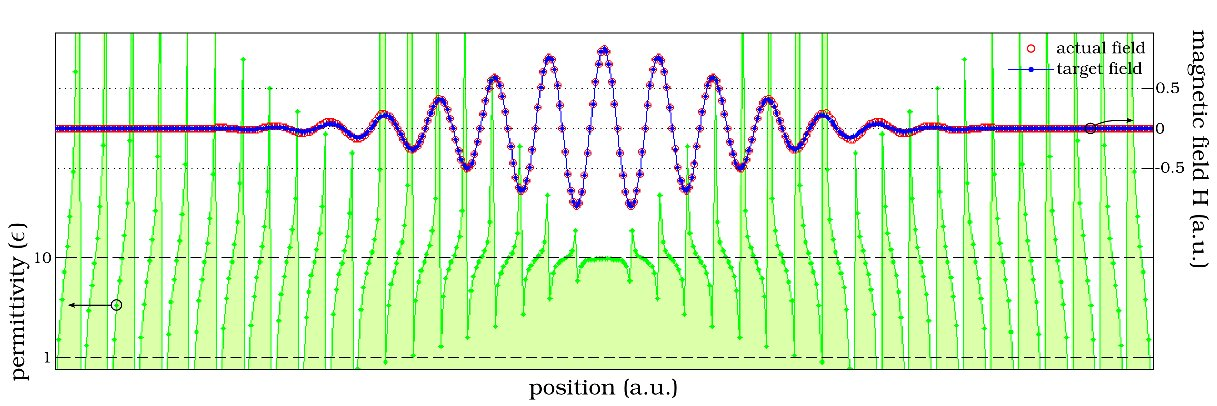
\includegraphics[width=\textwidth]{p1/leastsquares}
\caption{Inverse design of a one-dimensional structure using the unmodified least-squares method. The target field is a sinusoid within a Gaussian envelope. The computed dielectric structure (green area) supports a field (red circles) that exactly matches the target field (blue line). The entire design process is also extremely fast and takes less than $1$ second to complete on a generic desktop computer~\cite{mycomp}. The periodic singularities in the dielectric structure are non-physical and will be addressed later in the article.}
\label{ls pic}\end{figure}
The result of applying this method to a simple one-dimensional problem is shown in Fig.~\ref{ls pic}. A generic least-squares solver~\cite{cholmod} was used to find the dielectric structure, $y$ (green region), that exactly produces the target field, $x$ (blue line), using eq.~\eqref{lin ev}. Using a generic desktop computer, the solution was obtained in less than a second. Then a finite-difference time-domain (FDTD) solver was used to obtain the actual field (red circles) produced by the structure and to verify the accuracy of $y$.  

As expected, Fig.~\ref{ls pic} shows that the target field is reproduced exactly by the dielectric structure. However, the resulting structure is full of undesireable singularities. The rest of the section focuses on producing a well-behaved dielectric structure that still reproduces the target field accurately.

\subsection{Regularized Least-Squares}
The simplest way to produce a well-behaved dielectric structure is to add a regularization term to our least-squares problem, 
% \begin{equation}
% \begin{bmatrix} B \\ \sqrt{\eta} I \end{bmatrix} y = \begin{bmatrix} d \\ \sqrt{\eta}y_0 \end{bmatrix}
% \label{regls}\end{equation}
which is equivalent to solving the following optimization problem
\begin{equation}
\minimize_{y}\quad \|By-d\|^2 + \eta\|y-y_0\|^2.
\label{regls alt} \end{equation}
Here $y_0$ represents some initial guess for the dielectric structure, which we want the values of $y$ to stay close to, and $\eta>0$ is a parameter used to trade off fit, i.e. $\|By-d\|^2$, and deviation from $y_0$, i.e. $\|y-y_0\|^2$.

We chose to constrain $\epsilon$ around a constant value of $\epsilon_0 = 10$ and solved the least-squares system for $\eta=10^{-8}$, $10^{-6}$, and $10^{-4}$. The results, each still obtained in under a second, are shown in Fig.~\ref{regls pic} and illustrate the trade-off between constraining $\epsilon$ and accurately reproducing $H$.

\begin{figure}[htbp]\centering
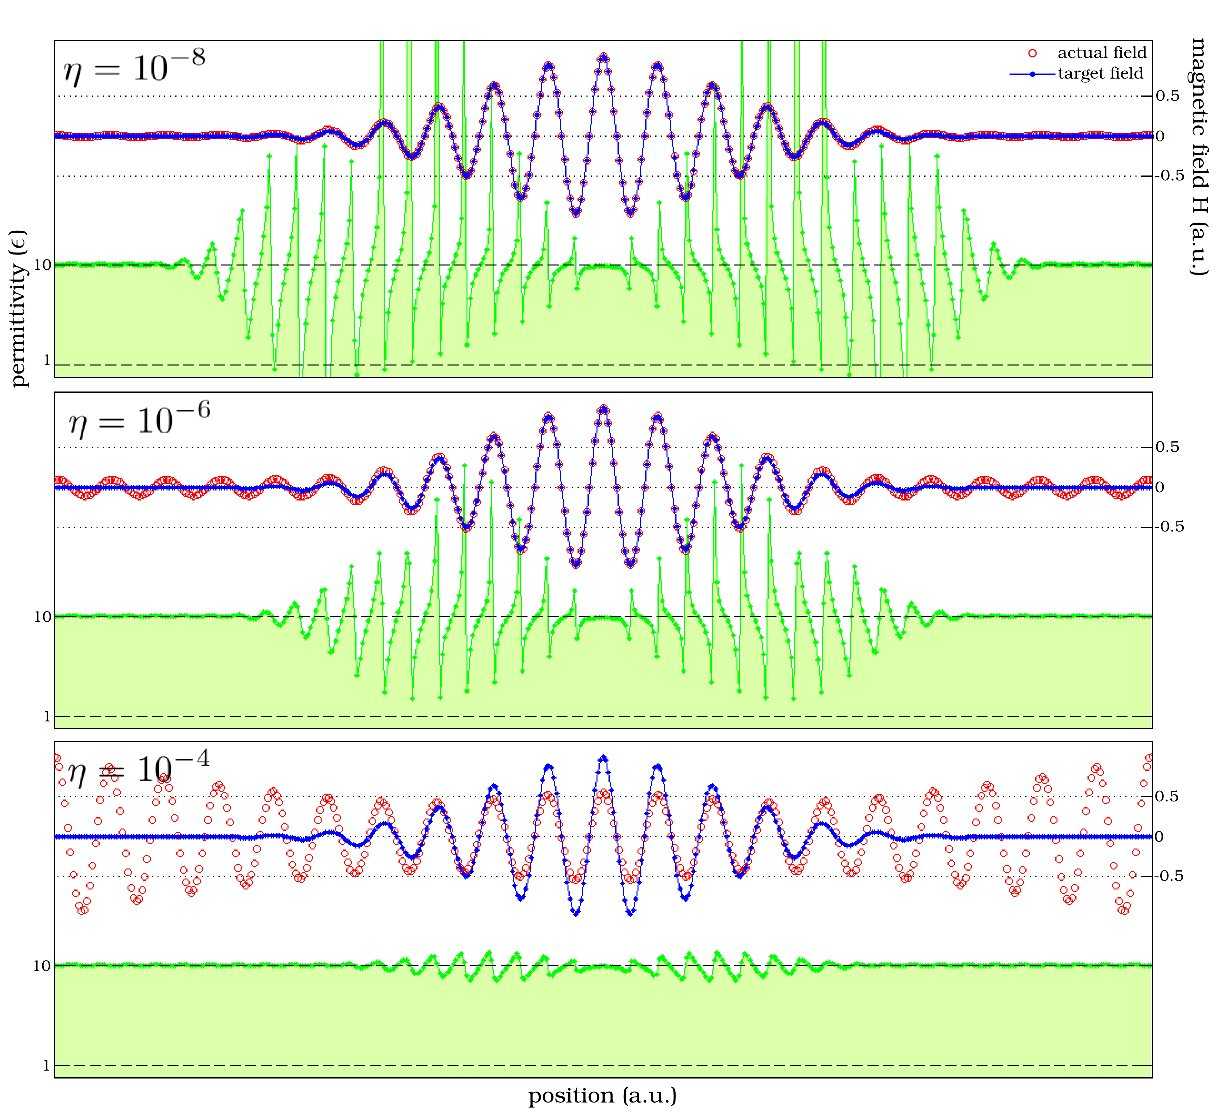
\includegraphics[width=\textwidth]{p1/regularized}
\caption{Inverse design of one-dimensional structures using the regularized least-squares method. The same target field is used as in Fig.~\ref{ls pic}, and the computation time remains below $1$ second. As the regularization parameter, $\eta$, is increased, $\epsilon$ is increasingly constrained to a chosen constant value of $10$. At the same time, the mismatch between target and actual fields increases markedly. This illustrates the apparent trade-off between producing reasonable structures and accurately reproducing a fixed target field.}
\label{regls pic}
\end{figure}

\chapter{Iterative design} \label{iterative}
% \section{Motivation for a Complementary Optimization Strategy}
The fundamental problem in the examples 
    in chapters \ref{direct} and \ref{regularized}
    is actually not in the methods themselves, 
    but in the improper selection of a target field. 
In fact, it is very difficult to select a suitable target field 
    because not every field even has a manufacturable dielectric structure 
    that is able to reproduce it. 
Furthermore, it is nearly impossible to select a multi-dimensional field 
    which corresponds to a well-behaved, isotropic and 
    discretely-valued $\epsilon$, 
    as would be needed for practical structures. 

What we realized was that a successful method 
    must be allowed to modify the target field as well as 
    its dielectric structure.
This realization led us to an iterative design strategy for nanophotonic devices.

\section{Problem formulation}
We start with the same target field as in the previous examples 
    but we now allow for it to be modified during the design process. 
Specifically, we alternate between modifying $z$ (structure) 
    to better fit $x$ (field), 
    and then modifying the $x$ (field) to better fit $z$ (structure):
    \begin{subequations}\begin{align} 
    \minimize_z & \|A(z)x - b\|^2 + \eta_0\|z - z_\text{prev}\|^2 \\
    \minimize_x & \|A(z)x - b\|^2 + \eta_1\|x - x_\text{prev}\|^2,
    \end{align}\end{subequations}
which can be more succintly expressed as 
    \BE \minimize_\text{alternately $x$ then $z$} 
        \|A(z)x - b\|^2 + \eta_0\|z - z_\text{prev}\|^2
                        + \eta_1\|x-x_\text{prev}\|^2. \label{iterative problem}\EE

In this formulation, both structure ($z$) and field ($x$) variables
    have regularization terms.
In order to avoid the performance/manufacturability trade-off 
    encountered in chapter~\ref{regularized},
    we decrease the values of $\eta_0$ and $\eta_1$ at each subsequent iteration.

\section{Implementation}
The most notable implementation difference is that,
    in contrast to direct design,
    \eq{iterative problem} must be solved multiple times
    in order to arrive at a good design.
Thus, design times now increase from seconds to minutes.

Note that, in order to design two-dimensional structures,
    \eq{iterative problem} is only modified in the
    definition of its constituent vectors and matrices,
    the formulation remains the same.


\section{Results}
\subsection{1D}
Fig.~\ref{comp pic} shows that the iterative algorithm, after $400$ iterations and with the correct choice of regularization parameters $\eta_0$ and $\eta_1$, results in a well-behaved structure that is able to closely reproduce the modified target field\cite{Lu10}. 

\begin{figure}[htbp]\centering
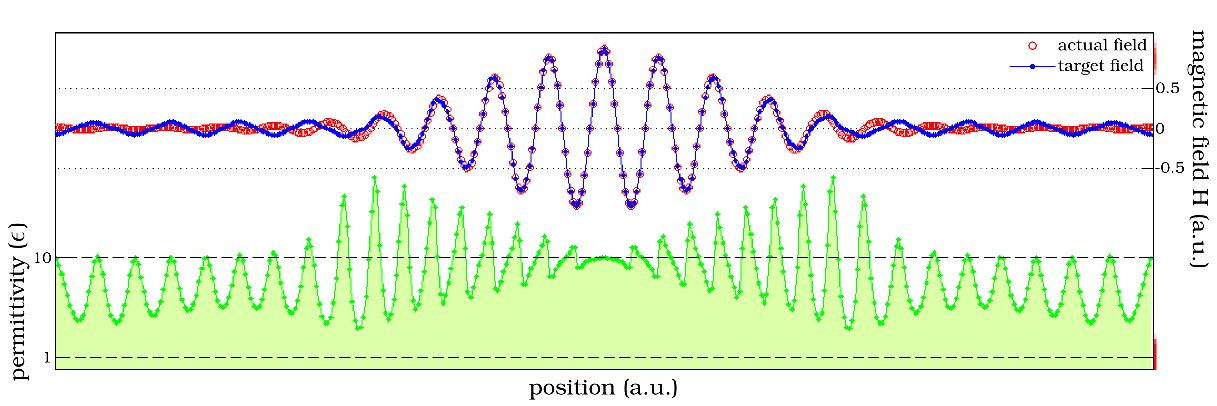
\includegraphics[width=\textwidth]{p1/complementary}
\caption{Iterative design of a one-dimensional resonator. 
    The target field in Figs \ref{p1:direct} and \ref{regls pic} is used as the initial target field. The rates of change for both $\epsilon$ and $H$ are controlled by regularization parameters $\eta_0=10^{-4}$ and $\eta_1=10^{-3}$ respectively. The $400$ iterations used to achieve this result took $60$ seconds to compute. This method results in a well-behaved $\epsilon$ that actually produces a field very similar to the original target field. Interestingly, the formation of a ``steady-state'' periodic structure toward the sides of the structure has emerged.}
\label{comp pic}
\end{figure}

\subsection{2D}
The iterative design method can also be extended to two dimensions\cite{Lu10}.
We demonstrate this using an S-shaped target field 
    which is non-trivial to reproduce. 
The design result is shown in fig.~\ref{S pic}. 
    The resulting dielectric structure is continuous, unbounded and 
    contains very few singularities (white dots), 
    but the final target and actual fields match up well. 
Also, the computational cost remains quite reasonable; the $50$ iterations needed required only $5$ minutes of computation time. 
\begin{figure}\centering
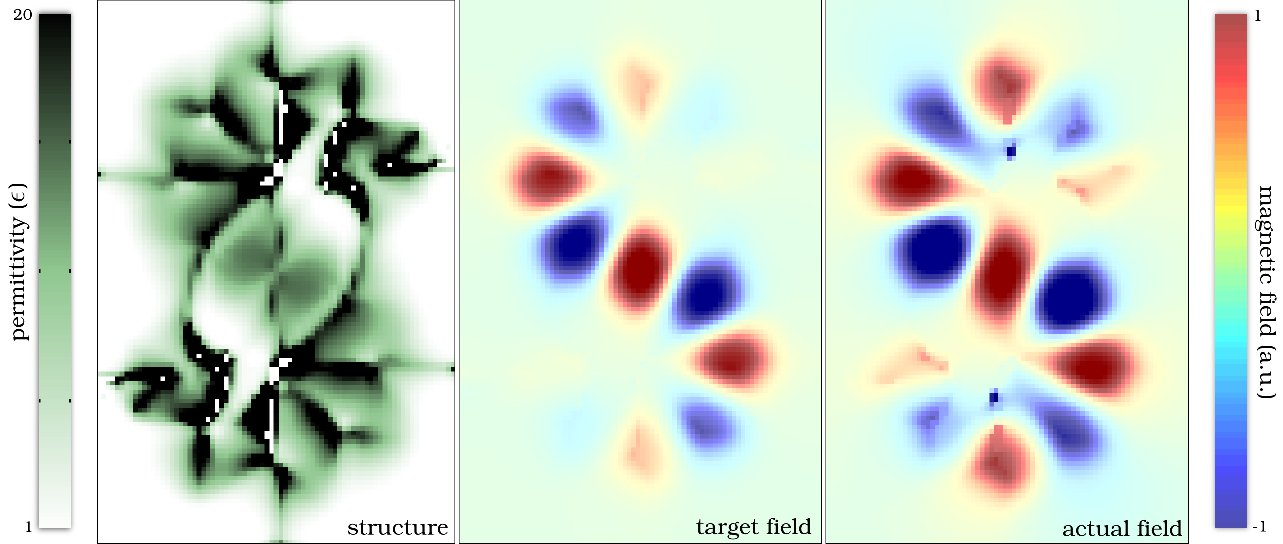
\includegraphics[width=\textwidth]{p1/S}
\caption{Iterative design of an ``S'' resonator. 
The design was initialized by specifying an initial dielectric structure ($\epsilon=1$ everywhere) and a resonant field in the shape of an ``S''. 
The final dielectric structure was produced after $50$ iterations which took $90$ seconds to complete in total. The grid size was $80\times 120$. The final dielectric structure is quite unintuive, and yet reproduces the target field surprisingly well. This example demonstrates the versatility of the iterative design method in producing designs, from very simple specifications, which otherwise could be attained only with considerable difficulty.}
\label{S pic}
\end{figure}

\chapter{Iterative design with bounded $\epsilon$} \label{bounded}
\section{Problem formulation}
In order to achieve a more practical, discretely-valued dielectric structure, we can impose strict upper- and lower-bounds on the structure ($z$). 
To this end, we can modify \eq{iterative problem} as such,
    \begin{subequations}
    \begin{align} 
    \minimize & \|A(z)x - b\|^2 + \eta_1\|x - x_\text{prev}\|^2\\
    \subto & z_\text{min} \le z \le z_\text{max}. 
    \end{align}\label{bounded problem}
    \end{subequations}
Here, the regularization term for $z$ has been replaced by hard constraints
    on the values that $z$ can take on.

This modification takes us one step closer to producing manufacturable structures,
    which must be discretely valued.

\section{Implementation} 
In this algorithm, \eq{bounded problem} is no longer linear in $z$
    but is still convex\cite{Boyd04}.
For this reason, the \emph{CVX} package\cite{Grant09}, 
    a Matlab-based modeling system for convex optimization, 
    is now used to solve \eq{bounded problem} for $z$.

\section{Results}
\subsection{1D}
Once again, we attempt the design of a one-dimensional resonator
    and find that a nearly binary-valued dielectric structure is obtained,
    as seen in fig.~\ref{bounded comp pic}\cite{Lu10}.
Note that the the directly discreteness of $z$ was not enforced (since that would make the problem non-convex); 
    however, a discrete, binary-valued structure arose fortuitously. 
Critically, this dielectric structure accurately produces the final target field. 

\begin{figure}[htbp]\centering
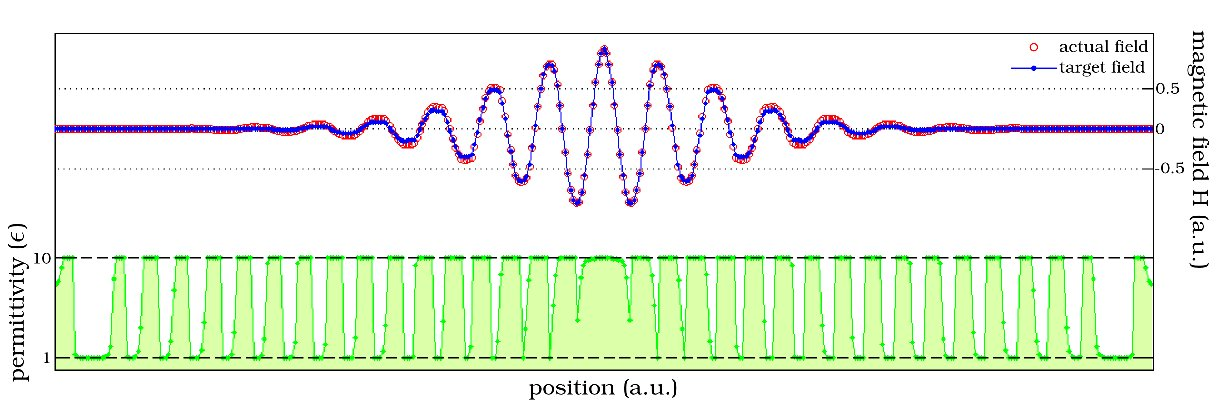
\includegraphics[width=\textwidth]{p1/bounded}
\caption{Iterative design of a one-dimensional structure with bounded $\epsilon$. 
    The parameters are identical to those used to produce Fig.~\ref{comp pic} with the exception that only one regularization term is now needed ($\eta_2=10^{-3}$). The algorithm was run for $100$ iterations, which took $100$ seconds. The structure turns out to be almost completely binary-valued and looks like a periodic structure with tapered duty cycle. It produces an actual field which very closely matches the final target field.}
\label{bounded comp pic}
\end{figure}

\subsection{2D}

We now use the complementary optimization method to design resonators with discrete, binary $\epsilon$ in two dimensions\cite{Lu10}.

Fig.~\ref{circle pic} shows the design of a circular grating resonator. 
The dielectric structure emerged from a very simple choice of initial structure, 
    namely a constant $\epsilon=12.25$ everywhere. 
The range of $\epsilon$ was limited to be from $1$ to $12.25$.
Additionally, the components of $\epsilon$ outside a specified circle 
    were held at a constant $\epsilon=12.25$ 
    for the duration of the design process. 
The entire algorithm was run for $40$ iterations and took $7$ minutes.
Interestingly, the central bowtie-like structure has emerged 
    from previous genetic optimization methods as well\cite{Gond08}. 

\begin{figure}[htbp]\centering
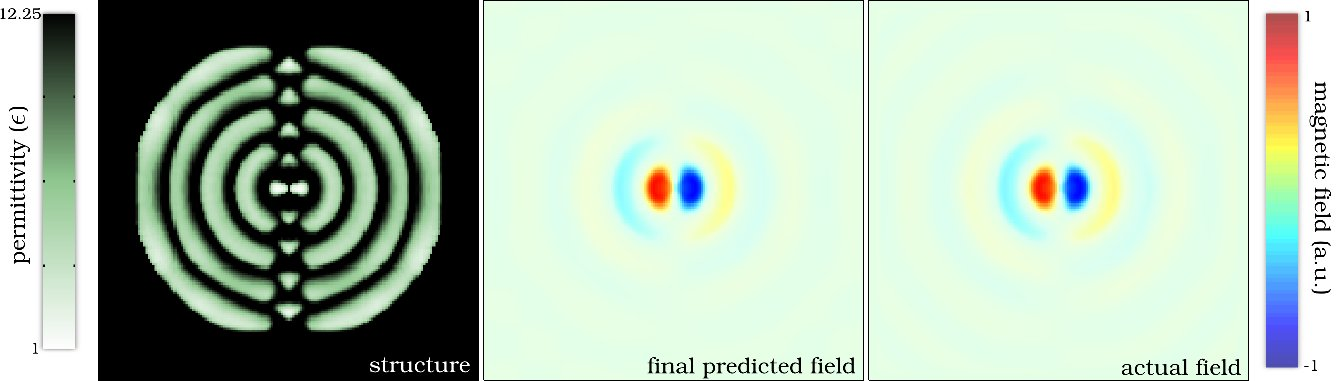
\includegraphics[width=\textwidth]{p1/circle}
\caption{Iterative design of a two-dimensional resonator 
            with hard constraints on $\epsilon$.
    The values of $\epsilon$ are only allowed to be modified within a central circular region and must be kept between $1$ and $12.25$. 
    After $40$ iterations on a $160 \times 160$ grid, which took $7$ minutes to complete, a discrete structure emerged with excellent match between the predicted ($x_{40}$) and actual fields. 
    The structure resembles a circular grating with a bowtie-like central structure for focusing the resonant energy to a single point.} 
\label{circle pic}
\end{figure}

The same approach was used to design a beam resonator 
    as shown in Fig.~\ref{line pic}. 
The parameters used in this design are identical 
    to those used for the circular resonator, 
    with the exception that the initial dielectric structure 
    now consists of an unbroken waveguide, 
    and the region where $\epsilon$ can be modified is now confined 
    to the center of the waveguide.

\begin{figure}[htbp]\centering
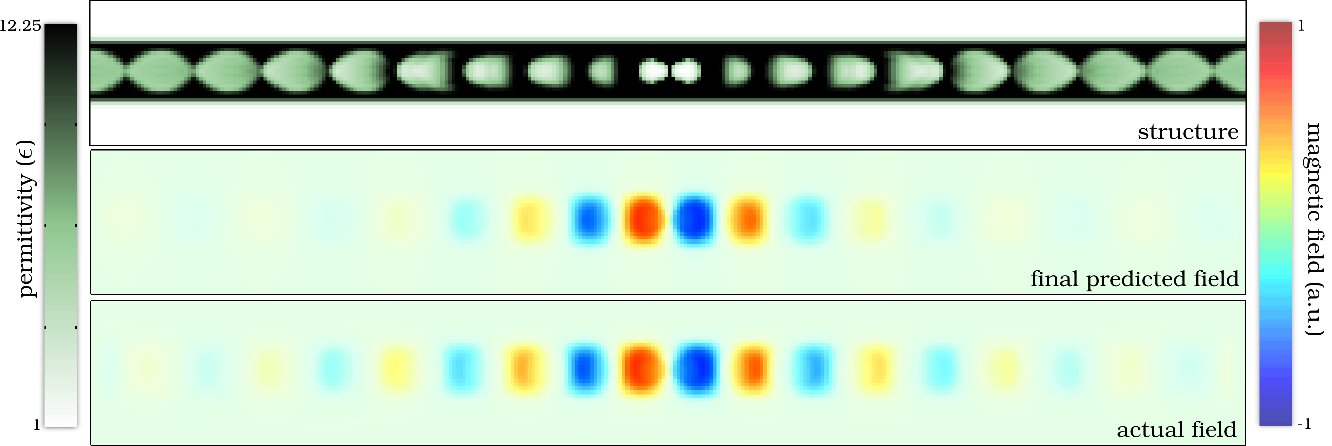
\includegraphics[width=\textwidth]{p1/beam}
\caption{Iterative design of a beam resonator in two dimensions 
        with bounded $\epsilon$. 
    The initial conditions are identical to those for Fig.~\ref{circle pic}, 
        except that the initial dielectric structure is an unbroken waveguide, 
        and $\epsilon$ can only be modified within that waveguide. 
    The structure emerged after $40$ iterations on a $320\times 40$ grid, 
        which took $5$ minutes of computation. 
    The bowtie-like structure has reappeared in the center.}
\label{line pic}
\end{figure}






% 
% \documentclass[10pt,letterpaper]{article}
% \usepackage{opex3}
% \usepackage{amsmath}
% \usepackage{graphicx}
% 
% \begin{document}
% \title{Inverse design of a three-dimensional nanophotonic resonator}
% \author{Jesse Lu, Stephen Boyd, and Jelena Vu\v{c}kovi\'{c}}
% \address{Stanford University, \\ Stanford, C.A., 94305}
% \email{jesselu@stanford.edu}
% 
% 
% \begin{abstract} 
% The inverse design of a three-dimensional nanophotonic resonator is presented. The design methodology is computationally fast (10 minutes on a standard desktop workstation) and utilizes a 2.5-dimensional approximation of the full three-dimensional structure. As an example, we employ the proposed method to design a resonator which exhibits a mode volume of $0.32(\lambda/n)^3$ and a quality factor of $7063$. % 8808 35648
% \end{abstract}
% 
% \ocis{(230.5750) Resonators.} % REPLACE WITH CORRECT OCIS CODES FOR YOUR ARTICLE
% 
% %%%%%%%%%%%%%%%%%%%%%%% References %%%%%%%%%%%%%%%%%%%%%%%%%
% \begin{thebibliography}{99}
% \bibitem{miller} D. A. B. Miller, ``Rationale and challenges for optical interconnects to electronic chips,'' Proc. of the IEEE \textbf{88}, 728-749 (2000).
% \bibitem{prevwork} J. Lu and J. Vuckovic, ``Inverse design of nanophotonic structures using complementary convex optimization,'' Opt. Express \textbf{18}, 3793-3804 (2010).
% \bibitem{inan} U. Inan, A. Inan, \emph{Electromagnetic Waves} (Prentice Hall, 2000), page 296.
% \bibitem{yee} K. Yee, ``Numerical solution of initial boundary value problems involving maxwell's equations in isotropic media,'' IEEE Trans. Antennas Propag. Mag. \textbf{14}, 302-307 (1966).
% \bibitem{boydbook} S. Boyd and L. Vandenberghe, \emph{Convex Optimization} (Cambridge University Press, 2004).
% \bibitem{altdir} S. Boyd, N. Parikh, E. Chu, B. Peleato, and J. Eckstein are preparing a manuscript to be called, ``Distributed Optimization and Statistical Learning via the Alternating Direction Method of Multipliers,'' \verb+http://www.stanford.edu/~boyd/papers/distr_opt_stat_learning_admm.html+. 
% \bibitem{cholmod} Y. Chen, T. A. Davis, W. W. Hager, and S. Rajamanickam, ``Algorithm 887: CHOLMOD, supernodal sparse Cholesky factorization and update/downdate,'' ACM Trans. Math. Software \textbf{35}, No. 3, 2009.
% \bibitem{cvx} M. Grant and S. Boyd, \emph{CVX: Matlab software for disciplined convex programming}, version 1.21. \verb+http://cvxr.com/cvx+, January 2011.
% \bibitem{digitize} D. Englund, I. Fushman, and J. Vuckovic, ``General recipe for designing photonic crystal cavities,'' Opt. Express \textbf{13}, 5961-5975 (2005).
% \end{thebibliography}
%  
% %%%%%%%%%%%%%%%%%%%%%%%%%%  body  %%%%%%%%%%%%%%%%%%%%%%%%%%
% \section{Begin of 2.5 D (Motivation)}
% To date, the design of nanophotonic devices has generally involved a lengthy (days, weeks) process in which one perturbs, by trial-and-error, canonical structures such as photonic crystals or waveguide-coupled rings to achieve the desired performance for the device. 
% 
% Instead, an inverse design method in which the user only specifies the desired electromagnetic field, or characteristics thereof, and then leaves the computer to find a dielectric structure satisfying these requirements, would be a much more intuitive and computationally efficient design strategy. Furthermore, such a method may even be the only feasible option available for the design of more complex multi-wavelength and multi-functional nanophotonic devices needed for on-chip integration\cite{miller}.
% 
\subsection{2.5D}
% \section{2.5-dimensional approximation}
Unfortunately, to directly extend our previous method to full three-dimensional space requires solving for a very large ($\sim 10^7 \times 10^7$) and ill-conditioned matrix, namely that given by the time-harmonic Maxwell's equation in three dimensions, which for the electric ($E$) field is
\begin{align}
\nabla\times\nabla\times E - \mu\omega^2\epsilon E &= 0,\quad\text{where}\label{wave} \\
E &= E(x,y,z).
\end{align}

Therefore, to make our problem more tractable, we formulate a 2.5-dimensional approximation of the electromagnetic fields of a planar three-dimensional nanophotonic device\cite{Lu11}. As shown in Fig.~\ref{approx}a, this involves treating a planar three-dimensional nanophotonic device as a truncated holey fiber with identical dielectric structure. We take advantage of the planar nature of most nanophotonic devices in this way to produce a tractable, computationally-fast method. The $E$-field inside such a holey fiber is expressed as
\begin{equation}
E = E(x,y)e^{-i\beta z},
\end{equation}
where $\beta$ is the wave-vector along the fiber axis. Solving for Eq.~\ref{wave} now requires solving for a much smaller ($\sim 10^5 \times 10^5$) matrix, which can be accomplished using standard linear algebra packages. This simulation technique is thus very similar to a two-dimensional finite-difference frequency-domain solver.

As an example, in Fig.~\ref{approx}b, we compare the 2.5-dimensional electric field against the three-dimensional simulated electric field (at the central plane of the slab), given by a standard finite-difference time-domain (FDTD) software package, for an L3 photonic crystal resonator. We see that with the appropriate choice of $\beta$, which we obtain by fitting a sinusoid to the out-of-plane decay in the three-dimensional FDTD solution, our approximation captures most of the characteristics of the three-dimensional field at the center plane of the slab. 
\begin{figure}[hbt]
\centering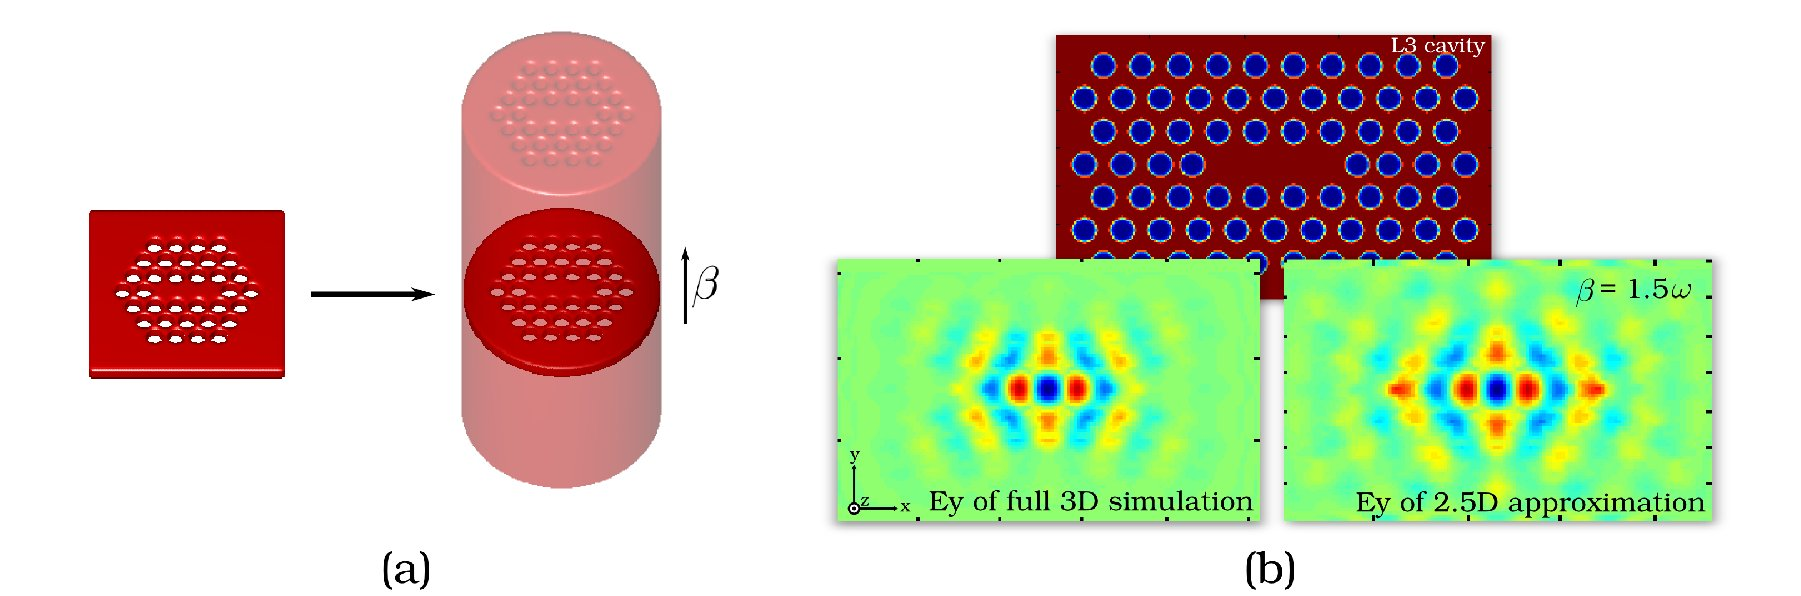
\includegraphics[width=\textwidth]{p2/approx}
\caption{(a) For computational feasibility, the resonant fields of a planar nanophotonic device are approximated as those of a truncated holey fiber with identical dielectric structure. (b) An example of our approximation using an L3 photonic crystal resonator. Most of the characteristics of the full three-dimensional field at the center of the slab appear in the approximate solution.}\label{approx}
\end{figure}

In this approximation, converting from a 2.5-dimensional structure to a full three-dimensional structure only requires the correct choice of slab thickness, $t$, since the in-plane values of $\epsilon$ remain the same. To estimate $t$ for the full three-dimensional device, we treat the resonant mode as a guided mode in a slab waveguide surrounded by a cladding of $n=1$. The expression for $t$ is then the thickness of the slab for the lowest-order TE mode of a slab waveguide with effective refractive index $n_\text{eff}$\cite{Inan00}:
\begin{align}
t &= \frac{2}{\beta}\tan^{-1}\frac{\alpha}{\beta},\label{t} \quad\text{where} \\
\alpha &= \sqrt{k_x^2 - \left(\frac{\omega}{c}\right)^2}, \quad\text{and} \\
k_x &= \sqrt{\left(\frac{n_\text{eff}\omega}{c}\right)^2 - \beta^2}.
\end{align}
Here, $\alpha$ is the wave-vector which determines the evanescent decay of the slab waveguide mode into air, while $k_x$ is an approximated in-plane k-vector. To determine $n_\text{eff}$, the effective refractive index, we use the following approximation,
\begin{equation}
n_\text{eff} = \sqrt{\frac{\|\epsilon E^2\|}{\|E^2\|}}.
\end{equation}
% In the above formulation and for the remainder of the manuscript, the norm ($\|\cdot\|$) refers to the 2-norm over the entire grid and is equivalent to the spatial integral $(\int | \cdot |^2 dr)^{1/2}$.

% 
% In our inverse design method, one proceeds by specifying either the resulting field or its characteristics and then computing a structure which will produce such a field. In this work, we chose to specify the desired field characteristics, namely, small mode-volume and large quality factor. The inverse design problem can then be formulated as,
% \begin{align}
% \text{minimize} \quad& \frac{\|\epsilon E^2\|}{\text{max}\{\epsilon E^2\}} \label{a1}\\ 
% \text{subject to} \quad 
%     & \nabla\times\nabla\times E - \mu\omega^2\epsilon E = 0 \label{a2}\\
%     & \nabla\cdot\epsilon E = 0 \label{adiv}\\
%     & \text{FT}_\text{lightcone}\{E\} = 0, \label{a3} \\
%     & \epsilon = \{\epsilon_\text{air}, \epsilon_\text{silicon}\} \label{a4}
% \end{align}
% where $\epsilon$ and $E$ are the permittivity and electric vector field respectively, defined within the 2.5-dimensional approximation and discretized along a standard Yee grid\cite{yee} with periodic boundary conditions. $\epsilon$ was constrained to be isotropic by only varying $\epsilon_z$ in each cell, and then determining $\epsilon_x$ and $\epsilon_y$ via spatial interpolation. $\text{FT}$ is the two-dimensional Fourier transform.
% 
% In this formulation, the minimization objective (Eq.~\ref{a1}) is the mode volume, which we desire to be as small as possible. Similarily, Eq.~\ref{a3} is a constraint on the electric field to produce a large quality factor by forbidding the existence of any Fourier components within the light cone. Eqs.~\ref{a2} and \ref{adiv} are physical constraints that $\epsilon$ and $E$ must satisfy, that is, the wave equation for the 2.5-dimensional fiber mode and the transversality condition. Lastly, Eq.~\ref{a4} is a binary constraint on epsilon, denoting that we only want the structure to be composed of air or silicon.
% 
% Although our 2.5-dimensional approximation has reduced the size and complexity of the matrices found in the above formulation, the form of the problem in Eq.~\ref{a1}-\ref{a4} is actually incredibly difficult to solve, if for no other reason that Eq.~\ref{a1}, \ref{a2}, and \ref{a4} are non-convex\cite{boydbook} for joint minimization on both $\epsilon$ and $E$. To make matters worse, the binary constraint in Eq.~\ref{a4} generally results in a problem which is NP-hard\cite{boydbook}. For these reasons, our strategy is to employ an alternating directions scheme\cite{altdir}, in which we break Eq.~\ref{a1}-\ref{a4} into two separate, tractable sub-problems which we then solve iteratively.
% 
% \subsection{Alternating directions: field optimization sub-problem}
% The first sub-problem in the alternating directions scheme involves optimizing $E$ while holding $\epsilon$ constant,
% \begin{align}
% \underset{E}{\text{minimize}} \quad& \|\nabla\times\nabla\times E - \mu\omega^2\epsilon E\|
%     + \eta \|\epsilon E^2\| \label{b1}\\ 
% \text{subject to} \quad 
%     & E_\text{center} = 1 \label{bcenter} \\
%     & \nabla\cdot\epsilon E = 0 \label{bdiv}\\
%     & \text{FT}_\text{lightcone}\{E\} = 0, \label{bQ}
% \end{align}
% which is a quadratic problem with linear equality constraints, and is easily solved using a standard factor-solve method for sparse matrices\cite{cholmod}.
% 
% In this sub-problem, the most significant modification to the original formulation in Eq.~\ref{a1}-\ref{a4} is that the constraint in Eq.~\ref{a2} has been relaxed and moved into the minimization objective (Eq.~\ref{b1}). We will denote this term ($\|\nabla\times\nabla\times E - \mu\omega^2\epsilon E\|$) as the \emph{physics residual}. 
% 
% At the same time, the term for the mode volume from Eq.~\ref{a1} has also been modified in Eq.~\ref{b1}. We denote this term ($\|\epsilon E^2\|$) as the \emph{design objective}. Note that although the denominator in the original formulation has been removed in order to make the term convex, the present formulation is still equivalent because we fix the $E$-field in the center of the structure (Eq.~\ref{bcenter}), where we want the maximum to occur. Also note that the constraint in Eq.~\ref{bcenter} is crucial in order to avoid the trivial solution $E=0$.
% 
% Lastly, the $\eta$ coefficient in Eq.~\ref{b1} allows us to trade-off between the physics residual and the design objective. Thus, in order to achieve a small mode volume, the initial value of $\eta$ is large and is subsequently exponentially reduced once per iteration at all points in the grid in order to bring the physics residual to 0. Furthermore, $\eta$ can also be given a spatial weighting in order to reduce in-plane losses; this strategy was implemented in the results presented here.
% 
% 
% \subsection{Alternating directions: structure optimization sub-problem}
% The second sub-problem in the alternating directions scheme involves optimizing $\epsilon$ while holding $E$ constant,
% \begin{align}
% \underset{\epsilon}{\text{minimize}} \quad& \|\nabla\times\nabla\times E - \mu\omega^2\epsilon E\| \label{c1} \\
% \text{subject to} \quad 
%     & \epsilon_\text{air} \le \epsilon \le \epsilon_\text{silicon}, \label{clim}
% \end{align}
% which is a quadratic problem with linear inequality constraints and is solved using CVX\cite{cvx}, a convex optimization package for Matlab.
% 
% As in the field optimization sub-problem, the physics residual has been relaxed and placed in the minimization objective (Eq.~\ref{c1}). However, we have chosen not to include the design objective term (mode volume). This modification was implemented as a heurestic that seemed to improve the aesthetic quality of the resulting structure.
% 
% The second major modification from the original formulation is found in the constraint in Eq.~\ref{clim}. Since the combinatorial problem given by the original constraint in Eq.~\ref{a3} proved to be intractable, the constraint on the values of $\epsilon$ is relaxed to allow for any value in the range from $\epsilon_\text{air}$ to $\epsilon_\text{silicon}$. The sub-problem is now relatively straightforward to solve, although it is very unlikely that one obtains a completely binary structure. In practice various digitization schemes can be implemented\cite{digitize}; however, such schemes were not needed here since a nearly binary structure was produced fortuitously.
% 
% \section{Result}
Using \eq{iterative problem}, along with our 2.5-dimensional approximation, the iterative design of a planar three-dimensional nanophotonic device is performed\cite{Lu11}.

In order to do so, the frequency, $\omega = 0.16 c/\Delta x$, and the out-of-plane wave vector, $\beta = 0.24 (\Delta x)^{-1}$, are chosen by the user. Here, $\Delta x$ is the grid spacing and $c$ is the speed of light in vacuum. Lastly, an initial dielectric structure consisting entirely of silion, $\epsilon = \epsilon_\text{silicon}$ everywhere on a $160 \times 160$ grid, is used as a starting point---although other initial structures (e.~g.~ air everywhere or random $\epsilon$) yield nearly identical structures in this case.

\begin{figure}[hbt]
\centering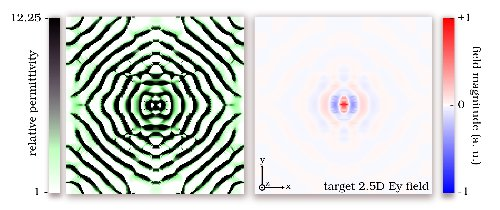
\includegraphics[width=\textwidth]{p2/target}
\caption{The (a) dielectric structure, $\epsilon$, and (b) target field, $E$ ($E_y$ shown only), produced after 75 iterations (10 minutes) on a $160\times 160$ grid. The resulting $\epsilon$ is almost completely binary, and relatively smooth.}\label{target}
\end{figure}
Figs.~\ref{target}a and \ref{target}b are the resulting values of $\epsilon$ and $E$ ($E_y$ shown only), respectively, after 75 iterations of our inverse design method. The entire inverse design process takes only 10 minutes on a standard desktop computer for the $160 \times 160$ grid. 

% The values of the physics residual and the design objective (mode volume) at each iteration are shown in Fig.~\ref{progress}. Most importantly, we see that the physics residual seems to converge linearly, indicating that the algorithm is reasonably efficient. The primary factor in determining this rate of convergence is the exponential decrease in $\eta$ (Eq.~\ref{b1}), since as $\eta$ decreases, increasing emphasis is placed on minimizing the physics residual in the field sub-problem. 
% 
% \begin{figure}[hbt]
% \centering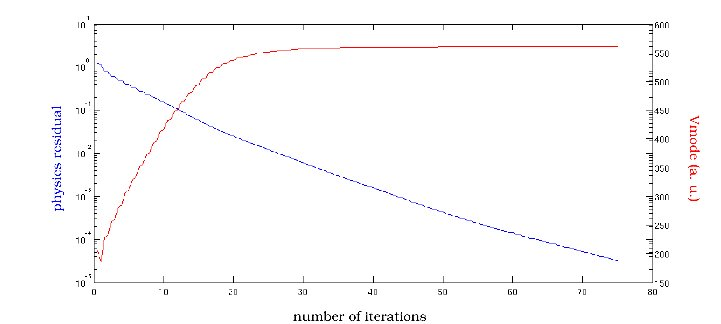
\includegraphics[width=\textwidth]{p2/the_prog}
% \caption{Value of the physics residual (blue) and design objective, or mode volume, (red) at each iteration. The physics residual seems to exhibit linear convergence, while the mode volume quickly saturates after roughly 25 iterations.}\label{progress}
% \end{figure}
% 
To evaluate the accuracy of our 2.5D approximation, we compared the field resulting from the iterations (target field) with the actual field of the resulting structure solved by the 2.5-dimensional approximation (2.5D fiber mode) as well as the field of a full three-dimensional FDTD simulation of the resulting structure (full 3D field), as shown in Figs.~\ref{comp} and \ref{xsec}.

As detailed above, the thickness of the corresponding three-dimensional structure is determined by Eq.~\ref{t}, which yielded a value of $8.16 \Delta x$. However, a small sampling of thicknesses in that vicinity resulted in a more accurate thickness of $8.5\Delta x$, which matched the resonant frequency of the target field and 2.5-dimensional fiber mode.
\begin{figure}[hbt]
\centering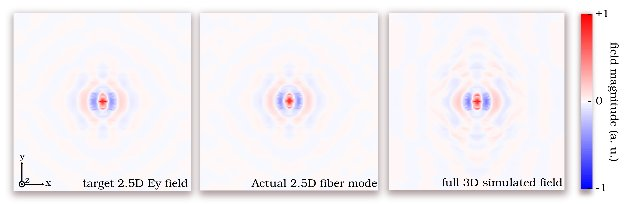
\includegraphics[width=\textwidth]{p2/compare}
\caption{Comparison ($E_y$) of (a) the target field from the inverse design method (from Fig.~\ref{target}), (b) the actual 2.5-dimensional fiber mode, and (c) the field from the full three-dimensional FDTD simulation. The target field matches well with the full three-dimensional field.}\label{comp}
\end{figure}

\begin{figure}[hbt]
\centering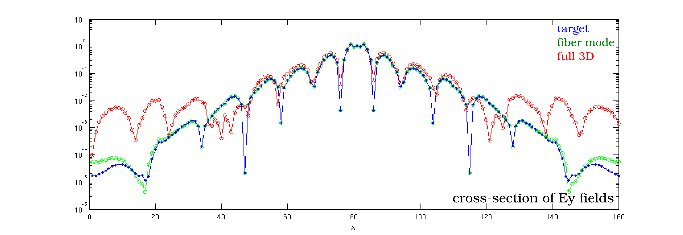
\includegraphics[width=\textwidth]{p2/the_xsec}
\caption{Comparison of the cross sections of the $E_y$ field along the x-axis from the target field (blue), the actual 2.5-dimensional fiber mode (green), and the field from the full three-dimensional FDTD simulation (red). There is some discrepancy between the target field and the full three-dimensional field, but even that is confined to the edges and is only on the order of $\sim 1\%$ of the maximum field amplitude.}\label{xsec}
\end{figure}
Fig.~\ref{comp} plots the $E_y$ component of the target field, 2.5-dimensional fiber mode and the full three-dimensional FDTD field side-by-side. Fig.~\ref{xsec} plots the horizontal cross sections of the magnitudes of the fields on a logarithmic scale. We see that the target field and fiber mode match very well, while there is significantly more discrepancy between the target field and the full three-dimensional field. This is expected with the use of our approximation; however, the error is still relatively small (below 1\% of the maximum field strength) and confined mostly to the edges of the structure.
% 
% \subsection{Performance}
% The fields from the full three-dimensional FDTD simulation were used to evaluate the performance of the device. The resulting mode volume was $0.32 (\frac{\lambda}{n})^3$ and the total quality factor was 7063. The radiative (out-of-plane) quality factor was 8808 and the in-plane quality factor was 35648.
% 
% Fig.~\ref{qcomp} shows the Fourier transforms of the target, fiber and three-dimensional $E_y$ fields taken at the center of the slab. Although there are virtually no field components in the light cone in the case of the target and fiber fields, additional components are present in the full three-dimensional case. This explains why even when leaky radiative components were strictly disallowed in the field optimization sub-problem, the error in the 2.5-dimensional approximation unavoidably introduces some leaky components in the case of the actual three-dimensional structure.
% 
% \begin{figure}[hbt]
% \centering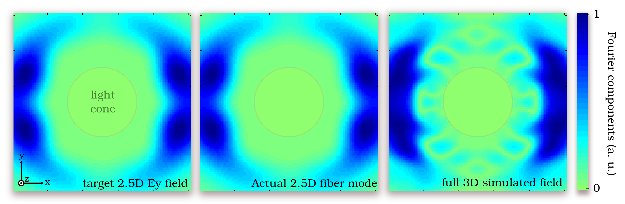
\includegraphics[width=\textwidth]{p2/qcomp}
% \caption{Comparison of the Fourier transforms of the $E_y$ fields of the (a) the target field from the inverse design method, (b) the actual 2.5-dimensional fiber mode, and (c) the field from the full three-dimensional FDTD simulation. The error in our approximation introduces some small additional Fourier components into the light cone.}\label{qcomp}
% \end{figure}
% 
% \section{Conclusion}
% In summary, by using a 2.5-dimension approximation, we demonstrate the inverse design of a three-dimensional nanophotonic resonator. Further development of our method includes applying our inverse method to design three-dimensional devices which support multiple fields at different frequencies. This includes resonant devices such as a multi-wavelength cavity, as well as waveguiding devices such as $N$-port couplers, multiplexers, and grating couplers.\\
% 

% 
% \documentclass[letterpaper,10pt]{article}
% \usepackage{graphicx}
% \usepackage{opex3}
% \usepackage{amsmath,amssymb}
% 
% 
% \begin{document}
% \title{Objective-first design of 
%     high-efficiency, small-footprint couplers between 
%     arbitrary nanophotonic waveguide modes}
% \author{Jesse Lu$^\ast$ and Jelena Vu\v{c}kovi\'{c}}
% \address{Stanford University, Stanford, California, USA.}
% \email{jesselu@stanford.edu}
% 
% \begin{abstract}
% We present an algorithm for designing
%     high efficiency ($\sim$98\%), 
%     small-footprint (1.5-4 square vacuum wavelengths)
%     couplers between arbitrary nanophotonic waveguide modes
%     in two dimensions.
% Our ``objective-first'' method is
%     computationally fast (15 minutes on a single-core personal computer), 
%     requires no trial-and-error, and
%     does not require guessing a good starting design.
% We demonstrate designs for various coupling problems which suggest 
%     that our method allows for the design of any 
%     single-mode, linear optical device.
% \end{abstract}
% \ocis{230.75370, 130.3990.}
% 
% \begin{thebibliography}{99}
% \bibitem{fibergrating} Y. Tang, Z. Wang, L. Wosinski, U. Westergren, and S. He,
%     ``Highly efficient nonuniform grating coupler for silicon-on-insulator 
%     nanophotonic circuits,''
%     Opt. Lett. \textbf{35}, 1290-1292 (2010).
% \bibitem{ridge}  K. K. Lee, D. R. Lim, L.C. Kimerling, J. Shin, and F. Cerrina, 
%     ``Fabrication of ultralow-loss Si/SiO2 waveguides by roughness reduction,''
%     Opt. Lett. \textbf{26}, 1888-1890 (2001).
% \bibitem{pcslow} Y. A. Vlasov, M. O'Boyle, H. F. Hamann, and S. J. McNab,
%     ``Active control of slow light on a chip with photonic crystal waveguides,''
%     Nature \textbf{438}, 65-69 (2005).
% \bibitem{slotfocus} M. Lipson, 
%     ``Guiding, modulating, and emitting light on 
%     silicon-challenges and opportunities,'' 
%     J. Lightwave Technol. \textbf{23}, 4222-4238 (2005).
% \bibitem{active} J. Van Campenhout, P. Rojo Romeo, P. Regreny, C. Seassal, 
%     D. Van Thourhout, S. Verstuyft, L. Di Cioccio, J.-M. Fedeli, 
%     C. Lagahe, and R. Baets, 
%     ``Electrically pumped InP-based microdisk lasers integrated with a 
%     nanophotonic silicon-on-insulator waveguide circuit,'' 
%     Opt. Express \textbf{15}, 6744-6749 (2007).
% \bibitem{metallic} L. Tang, S. E. Kocabas, S. Latif, A. K. Okyay, 
%     D. S. Ly-Gagnon, K. C. Saraswat, and D. A. B. Miller, 
%     ``Nanometre-scale germanium photodetector enhanced by a 
%     near-infrared dipole antenna,'' 
%     Nature Photonics \textbf{2}, 226-229 (2).
% % \bibitem{fwadia} V. R. Almeida, R. R. Panepucci, and M. Lipson, 
% %     ``Nanotaper for compact mode conversion,'' 
% %     Opt. Lett. \textbf{28}, 1302-1304 (2003) 
% % \bibitem{wwadia} S. G. Johnson, P. Bienstman,  M. A. Skorobogatiy, 
% %     M. Ibanescu1, E. Lidorikis, and J. D. Joannopoulos,
% %     ``Adiabatic theorem and continuous coupled-mode theory for 
% %     efficient taper transitions in photonic crystals,''
% %     Phys. Rev. E \textbf{66}, 066608 (2002)
% % \bibitem{deriv} F. Wang, J. S. Jensen, O. Sigmund, 
% %     ``Robust topology optimization of photonic crystal waveguides with 
% %     tailored dispersion properties.'' 
% %     J. Opt. Soc. Am. B \textbf{28}, 387-397 (2011)
% % \bibitem{boydbook} S. Boyd, and L. Vandenberghe, 
% %     \emph{Convex Optimization} 
% %     (Cambridge University Press, 2004)
% \bibitem{prevwork} J. Lu, S. Boyd, and J. Vuckovic, 
%     ``Inverse design of a three-dimensional nanophotonic resonator,''
%     Opt. Express \textbf{19}, 10563-10750 (2011). 
% \bibitem{veronis} G. Veronis, and S. Fan, 
%     ``Theoretical investigations of compact couplers between dielectric slab 
%     waveguides and two-dimensional metal-dielectric-metal plasmonic waveguides,'' 
%     Opt. Express \textbf{15}, 1211-1221 (2007).
% \bibitem{yang} R. Yang, R. A. Wahsheh, Z. Lu, and M. A. G. Abushagur, 
%     ``Efficient light coupling between dielectric slot waveguide and plasmonic
%     slot waveguide,'' Opt. Lett. \textbf{35}, 649-651 (2010).
% \bibitem{code} \url{www.github.com/JesseLu/objective-first}
% \end{thebibliography}
% 
\chapter{Objective-first design} \label{ob-1}
% 
% % Why is waveguide mode conversion important?
% Optical mode conversion, 
%     the efficient transfer of photons from one guided mode to another,
%     is a fundamental requirement in nanophotonics.
% For instance, efficient conversion between waveguides modes
%     is essential for:
%     \begin{itemize}
%         \item Coupling to and from optical fiber\cite{fibergrating}, 
%         to communicate with the outside world.
%     \item Coupling between various nanophotonic waveguides, 
%         since different waveguides are best suited for different applications.
%         For example, ridge waveguides seem ideal for 
%             low-loss transport\cite{ridge},
%             but other waveguides, 
%             such as photonic crystal waveguides or slot waveguides,
%             may be better suited for slow-light\cite{pcslow} 
%             or nonlinear optical devices based on 
%             localized field intensities\cite{slotfocus}.
%     \item Coupling between different materials systems such as
%        passive, active\cite{active}, and metallic\cite{metallic} devices. 
%     \end{itemize}
% In fact, the problem of converting between nanophotonic modes is essentially
%     the function of all linear nanophotonic devices, since
%     any linear device is completely characterized by its input and output modes
%     and the coupling coefficients between them.
% 
% In this paper, we present a method to solve the problem 
%     of designing single-mode, linear nanophotonic devices.
% We then demonstrate this method by designing coupling structures 
%     between various nanophotonic waveguides.
% Furthermore, we show that our method 
%      does not require a good initial design,
%      is computationally fast,
%      and can generate high efficiency couplers within a very small footprint. 
% 
% 
% % Why are current solutions insufficient?
% % Brute force
% Of the design strategies currently available,
%     brute-force parameter search is the most often employed 
%     because of its sheer simplicity.
% Although it may be suitable for tuning existing designs,
%     the parameter space for most practical devices is simply too large
%     for such a strategy to be tractable.
% 
% % Adiabatic mode conversion (large devices, symmetry breaking)
% Adiabatic mode conversion strategies have been succesful
%     for certain fiber-waveguide\cite{fwadia} and 
%     waveguide-waveguide\cite{wwadia} couplers,
%     even if the resulting devices often require large footprints.
% However, adiabatic approaches cannot be used in many important cases 
%     such as coupling in the out-of-plane direction, or
%     coupling between modes of opposite symmetry.

% How does your algorithm solve this problem?
% \subsection{Advantages of objective-first design}
% \section{Objective-first approach}
% % What is objective-first optimization?
% Physical structures are typically designed by solving the following problem:
%     \begin{subequations}\label{eq:adj}
%     \begin{align} 
%     \text{decrease} & \quad f(x) \label{eq:adj:obj} \\ 
%     \text{subject to} & \quad g(x,p) = 0, \label{eq:adj:con}
%     \end{align}
%     \end{subequations}
%     where $x$ is the field variable and $p$ is the structure variable.
% Here, $f(x)$, the \emph{design objective}, 
%     calculates the performance of the device 
%     (e.g. amount of power lost); 
%     while $g(x,p)$ is the underlying physical equation for the system
%     (e.g. the electromagnetic wave equation).
% 
% In contrast, the objective-first approach solves 
%     \begin{subequations}\label{eq:ob1}
%     \begin{align} 
%     \text{decrease} & \quad \|g(x,p)\|^2 \label{eq:ob1:obj} \\ 
%     \text{subject to} & \quad f(x) = 0, \label{eq:ob1:con}
%     \end{align}
%     \end{subequations}
%     where $\|g(x,p)\|^2$ is the \emph{physics residual}.
% We term this formulation ``objective-first''
%     because the design objective is prioritized even above satisfying physics;
%     specifically, we force our design to always exhibit the desired performance
%     ($f(x) = 0$), even at the expense of
%     not perfectly satisfying the underlying physics which governs its operation.
% 
% The motivation behind this formulation is two-fold.
% First, this approach allows one to arrive at a locally-optimal design rapidly 
%     by allowing $x$ and $p$ to vary independently, 
%     as opposed to Eq.~\ref{eq:adj}
%     where the value of $x$ is completely dependent on $p$.
% Second, it enables an increase in the likelihood of 
%     arriving at a high efficiency design
%     by forcibly imposing $f(x) = 0$,
%     and thereby circumvents any local optima consisting of
%     low-performance devices.
% 
% How is it applied to waveguide coupler design?
\section{Problem formulation}
Our next realization was that,
    for linear nanophotonic devices,
    only certain portions of the electromagnetic field were relevant 
    to device performance--namely the boundary fields
    at the input and output ports of the device.
This realization motivated the following problem formulation:
    \begin{subequations}
    \begin{align} 
    \minimize & \|A(z)x - b\|^2 \\
    \subto & x_\text{boundary} - \hat{x}_\text{boundary} = 0 \\
        & z_\text{min} \le z \le z_\text{max},
    \end{align} \label{ob1 problem}
    \end{subequations}
    which replaces the field regularization term from \eq{iterative problem}
    with the hard constraint $x_\text{boundary} - \hat{x}_\text{boundary} = 0$.
This constraint forces the field at the device boundary ($x_\text{boundary}$)
    to be equal to that of an ideal device ($\hat{x}_\text{boundary}$),
    as shown in fig.~\ref{fig:intro}.
We call this type of formulation ``objective-first''
    since the performance of the device is prioritized above
    the physicality of the device.

\begin{figure}[htb]
    \centering
    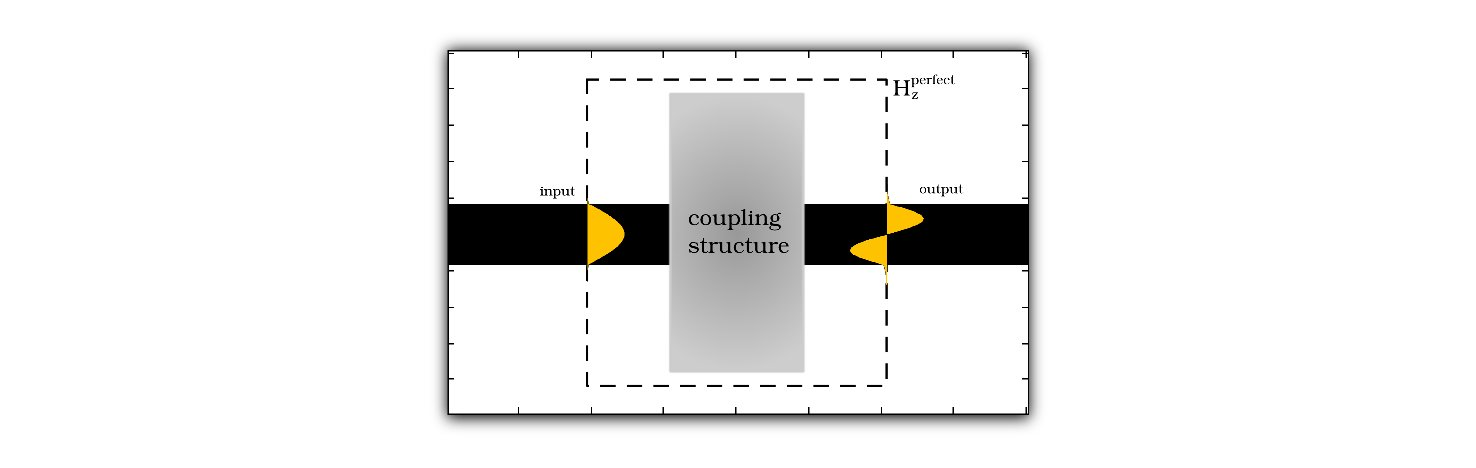
\includegraphics[width=\textwidth]{p3/intro} 
    \caption{Boundary-value formulation of the design objective.
        The values of $H_z^\text{perfect}$, 
            defined along the dashed box surrounding the design area
            (coupling structure), 
            are shown in orange. 
        The values of $H_z^\text{perfect}$ along the top and bottom edges
            of the dashed box are set to zero.
        In this schematic, the fundamental and second-order waveguide modes
            have been chosen as the input and output modes respectively.}
    \label{fig:intro}
\end{figure}
%\section{Objective-first design of waveguide couplers}
% We now demonstrate the objective-first approach
%     by designing waveguide couplers in two-dimensions.
% As such, we do not analyze effects which are only present in full 
%     three-dimensional systems, such as out-of-plane losses.
% Specifically, we work in the two-dimensional transverse electric mode,
%     choosing $H_z$ as the field variable $x$,
%     and $\epsilon^{-1}$ (the inverse of the permittivity) 
%     as the structure variable $p$.
% This results in the following form of the physics residual,
%     \begin{equation}
%     \|g(x,p)\|^2 = 
%     \|g(H_z, \epsilon^{-1})\|^2 = 
%     \| \nabla \times \epsilon^{-1} \nabla \times H_z - \mu_0 \omega^2 H_z \|^2,
%     \end{equation}
%     where $\omega$ is the angular frequency,
%     and $\mu_0$ is the permeability of free-space.
% 
% In order to produce a method applicable 
%     to the design of any linear nanophotonic device,
%     we note that its performance
%     will be completely characterized by the fields along its boundary,
%     and therefore, 
%     we choose a boundary-value formulation for the design objective 
%     as shown in Fig.~\ref{fig:intro}.
% Namely, we first compute the boundary fields needed to obtain
%     perfect performance, $H_z^\text{perfect}$,
%     and then form the design objective as
%     \begin{equation}
%     f(x) = f(H_z) = \begin{bmatrix}
%         H_z - H_z^\text{perfect} \\
%         \frac{\partial H_z}{\partial n} - 
%             \frac{\partial H_z^\text{perfect}}{\partial n}
%         \end{bmatrix}_\text{boundary}
%         = 0,
%     \end{equation}
%     where $\partial H_z / \partial n$ 
%     denotes the spatial derivative in the direction normal to the boundary.
% 
% \begin{figure}[htb]
%     \centering
%     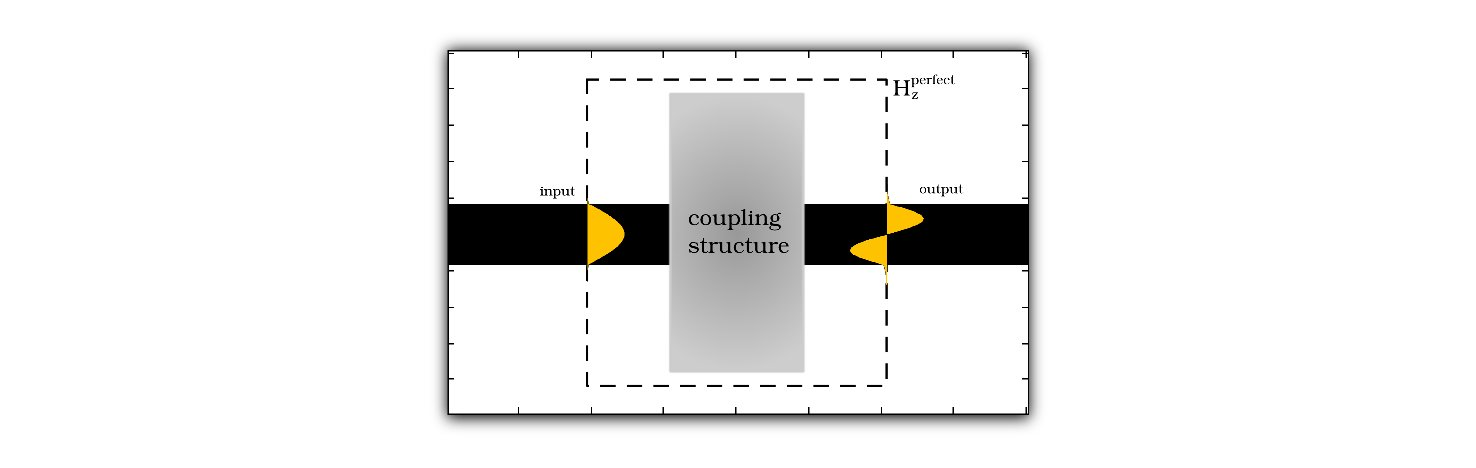
\includegraphics[width=\textwidth]{p3/intro} 
%     \caption{Boundary-value formulation of the design objective.
%         The values of $H_z^\text{perfect}$, 
%             defined along the dashed box surrounding the design area
%             (coupling structure), 
%             are shown in orange. 
%         The values of $H_z^\text{perfect}$ along the top and bottom edges
%             of the dashed box are set to zero.
%         In this schematic, the fundamental and second-order waveguide modes
%             have been chosen as the input and output modes respectively.}
%     \label{fig:intro}
% \end{figure}
%     
Such a design objective is both extremely simple and widely adaptable 
    to the design of linear nanophotonic devices in general\cite{Miller12}.
On the other hand, such a formulation often prohibits the physics residual 
    from disappearing completely; 
    however, we find that very good device performance is still obtained
    as long as the physics residual is sufficiently small.

\section{Implementation}
We employ an alternating directions strategy,
    where both $x$ and $z$ are solved iteratively
    and limit the allowable values of $\epsilon$ to be between
    the permittivity of vacuum and of silicon,
    \begin{equation}
    \epsilon_0 \le \epsilon \le \epsilon_\text{silicon}.
    \end{equation}
Note that a completely binary structure,
    where $\epsilon = \{\epsilon_0, \epsilon_\text{silicon}\}$,
    is needed for manufacturing purposes.
That said, the final designs presented here 
    all have significant portions which are already binary.

\section{Results}
We now demonstrate the objective-first approach
    by designing waveguide couplers in two-dimensions.
As such, we do not analyze effects which are only present in full 
    three-dimensional systems, such as out-of-plane losses.
Specifically, we work in the two-dimensional transverse electric mode,
    choosing $H_z$ as the field variable $x$,
    and $\epsilon^{-1}$ (the inverse of the permittivity) 
    as the structure variable $z$.

Specifically, we present five results which suggest our method
    is indeed able to design arbitrary single-mode, linear nanophotonic devices\cite{Lu12}.
These results comprise of couplers between 
    the following nanophotonic waveguides:
    \begin{enumerate}
    \item coupling between waveguides of different refractive index and width
        (Fig.~\ref{fig:fiber});
    \item coupling between waveguide modes of different order and symmetry
        (Fig.~\ref{fig:mode});
    \item coupling between waveguides that confine light 
        using different principles 
        (index guided vs. distributed Bragg reflection guided), 
        i.e., between a slab waveguide and a photonic crystal fiber
        (Fig.~\ref{fig:aircore})
    \item coupling from a dielectric to a plasmonic metal-insulator-metal 
        waveguide (Fig.~\ref{fig:mim}); and
    \item coupling from a dielectric waveguide to a (plasmonic) metal wire
        (Fig.~\ref{fig:wire}).
    \end{enumerate}
All the designs presented are both highly efficient 
    ($\sim 98\%$ coupling efficiency, in contrast to previous designs
    which achieve only $\sim 70\%$ coupling efficiency\cite{Veronis07,Yang10})
    and extremely compact 
    (with footprints of only 1.5-4 square vacuum wavelengths).

Note, however, that the small footprint of the designs presented does not 
    imply small, unresolvable feature sizes.
On the other hand, assuming a vacuum wavelength of 1550 nm,
    the smallest possible feature in any of the examples presented is still
    37 nm $\times$ 37 nm (see Fig.~\ref{fig:fiber}, for example),
    as given by the size of a single grid point;
    placing virtually all designs within reach of current-generation lithographic
    systems.

In addition, good starting points were not required; 
    all initial designs were simply $\epsilon = 9$ everywhere
    (a somewhat arbitrary guess, other values work as well).
Finally, only 15 minutes on a single-core personal computer
    were needed to obtain each design.

In appendix~\ref{ob-1 additional}, we further demonstrate the generality of our method
    by presenting several additional examples including
    \begin{enumerate}
    \item coupling between all four modes of a wide dielectric waveguide;
    \item coupling from a wide, low-index waveguide to the output waveguides in 
        Figs~\ref{fig:mode}-\ref{fig:wire}; and
    \item coupling to selected channels of a set of five plasmonic waveguides.
    \end{enumerate}

Furthermore, appendix~\ref{ob-1 meta} contains designs for metamaterial-like
    devices.

\begin{figure}[htb]
    \centering
    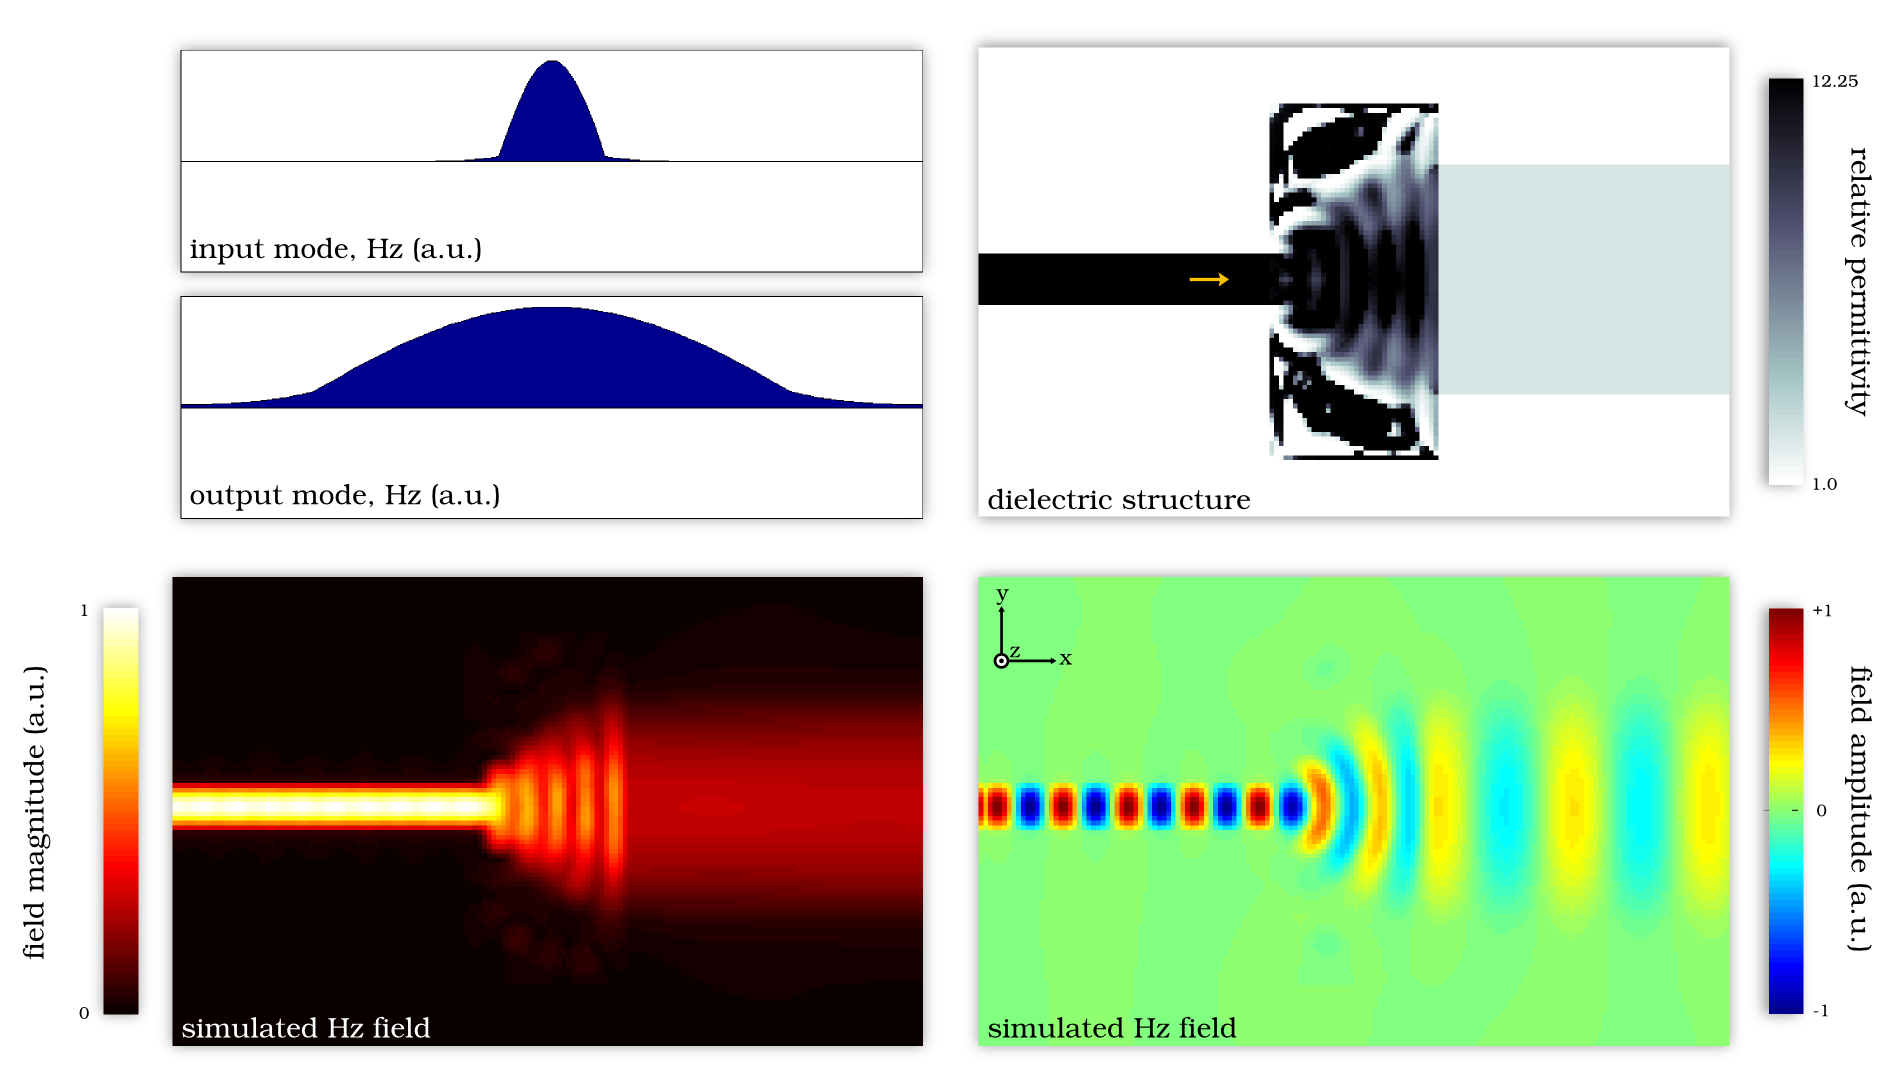
\includegraphics[width=\textwidth]{p3/1} 
    \caption{Coupler from a narrow, high-index ($\epsilon=12.25$) waveguide to
            a wide, low-index ($\epsilon=2.25$) waveguide. 
        The $H_z^\text{perfect}$ boundary values used as 
            the design objective are shown in the upper-left plots, 
            the generated structure is shown in the upper-right plot, and
            the simulated $H_z$ fields of the device are shown 
            in the bottom two plots.
        The computed efficiency of the coupler is high, $99.8\%$, and
            the device is also extremely compact, 
            convering only $36 \times 76$ grid points,
            where the vacuum wavelength is 42 grid points
            (footprint of $1.55$ square vacuum wavelengths).
        Computation time was 15 minutes on a personal computer.}
    \label{fig:fiber}
\end{figure}
\begin{figure}[htb]
    \centering
    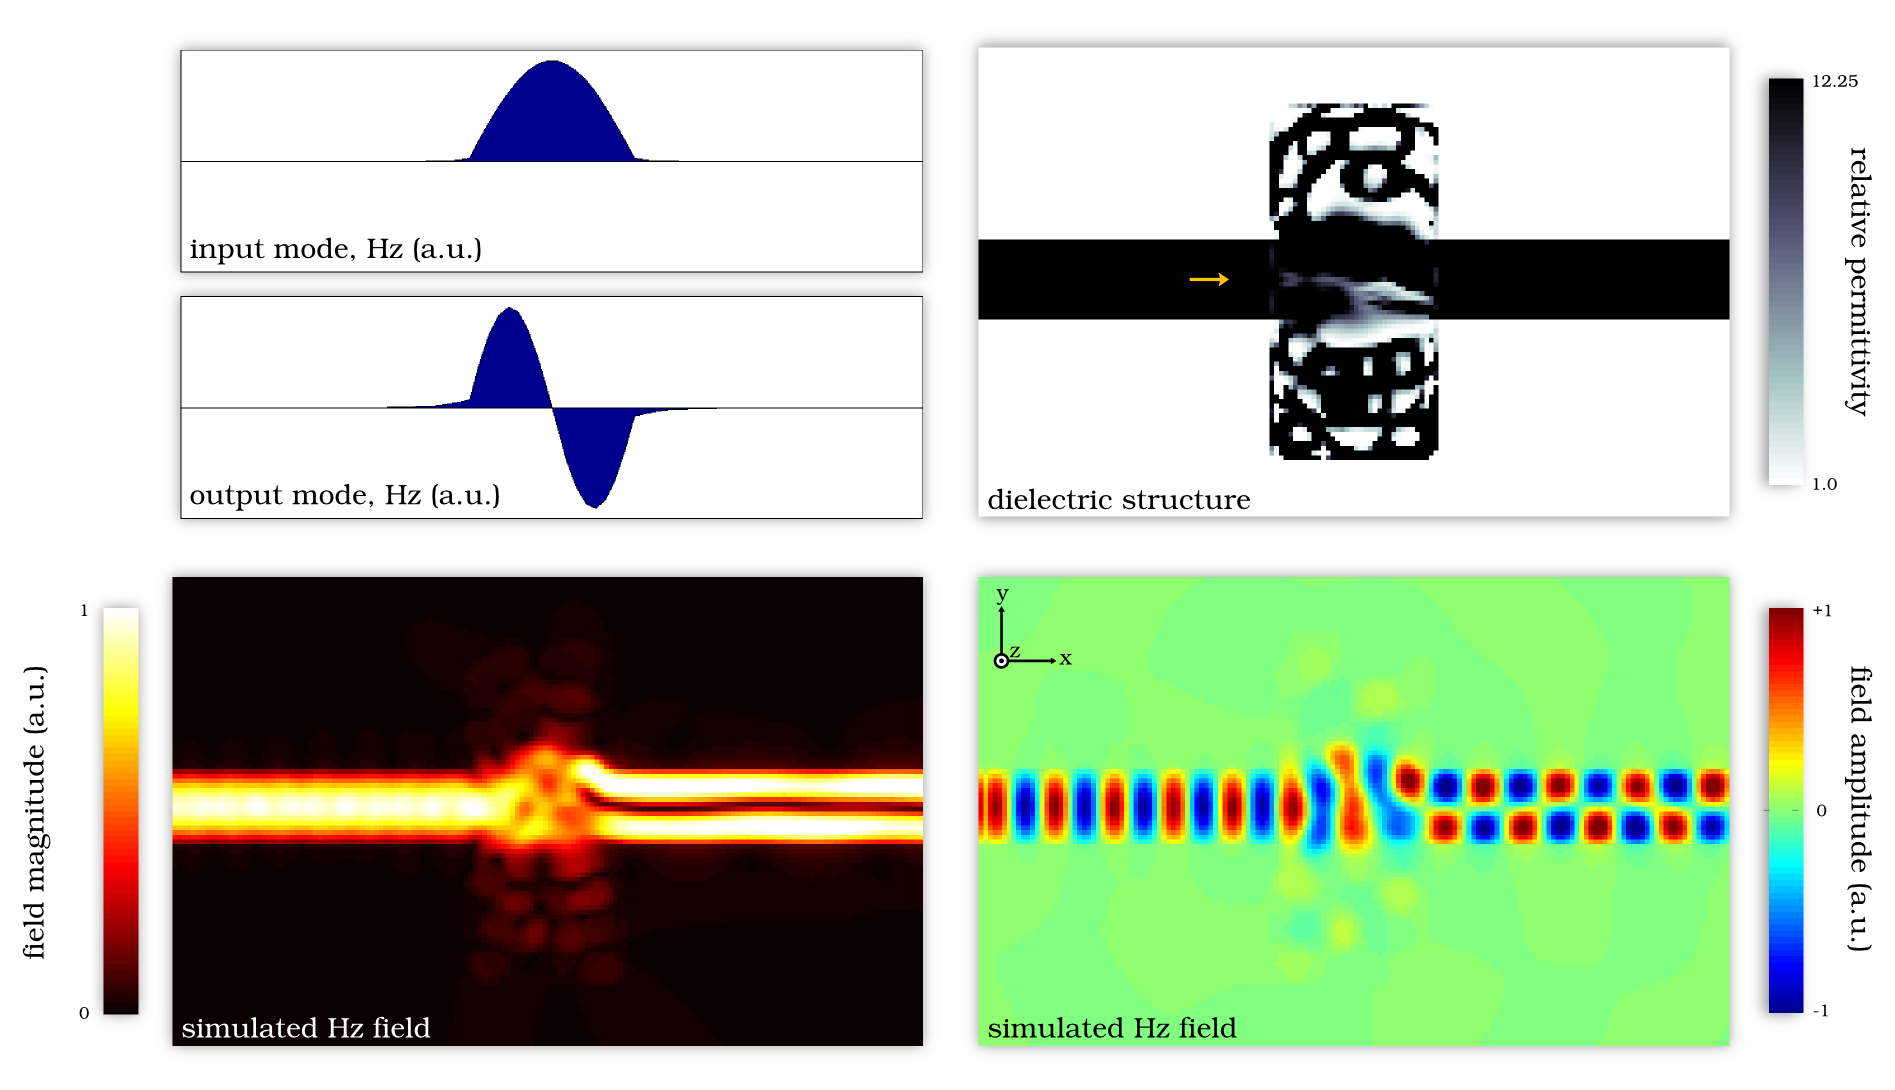
\includegraphics[width=\textwidth]{p3/2} 
    \caption{Coupler that converts the fundamental waveguide mode to the
            second-order waveguide mode.
        This problem is quite difficult since the two modes are of 
            opposite symmetry.
        For example, adiabatic approaches cannot be applied to this case.
        However, our method produces a device 
            (which has the same dimensions and vacuum wavelength as 
            Fig.~\ref{fig:fiber})  
            with a coupling efficiency of $98.0\%$. 
        Computation time was 15 minutes on a personal computer.
        }
    \label{fig:mode}
\end{figure}
\begin{figure}[htb]
    \centering
    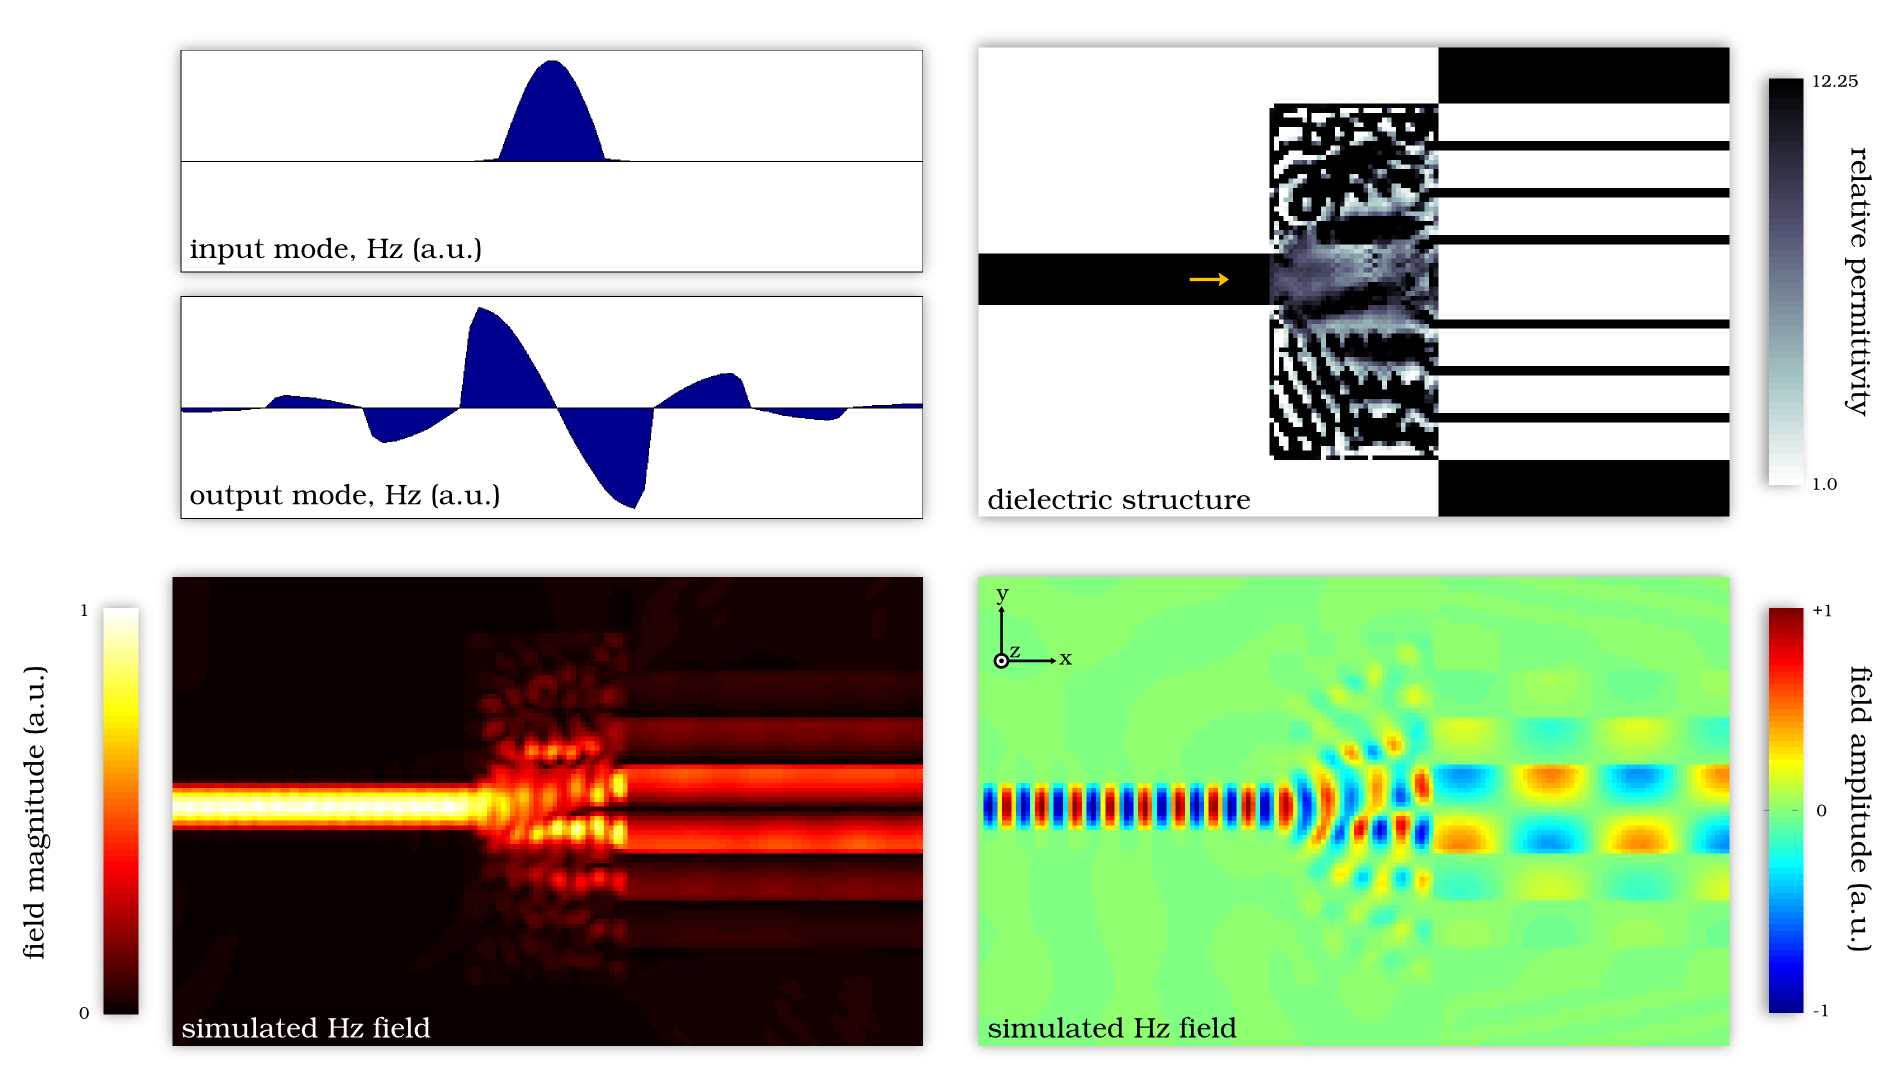
\includegraphics[width=\textwidth]{p3/3}
    \caption{Coupler between a dielectric slab waveguide to 
            an air-core waveguide.
        Here, not only are the modes of opposite symmetry,
            but the output waveguide operates on a fundamentally different
            principle (distributed reflection) than the input waveguide 
            (index guided).
        The device still achieves an efficiency of $98.9\%$, demonstrating the
            versatility of our method.
        The vacuum wavelength is 25 grid points, 
            while the device footprint is still $36 \times 76$ grid points
            (footprint of 4.38 square vacuum wavelengths).
        Computation time was 15 minutes on a personal computer.
        }
        \label{fig:aircore}
\end{figure}
\begin{figure}[htb]
    \centering
    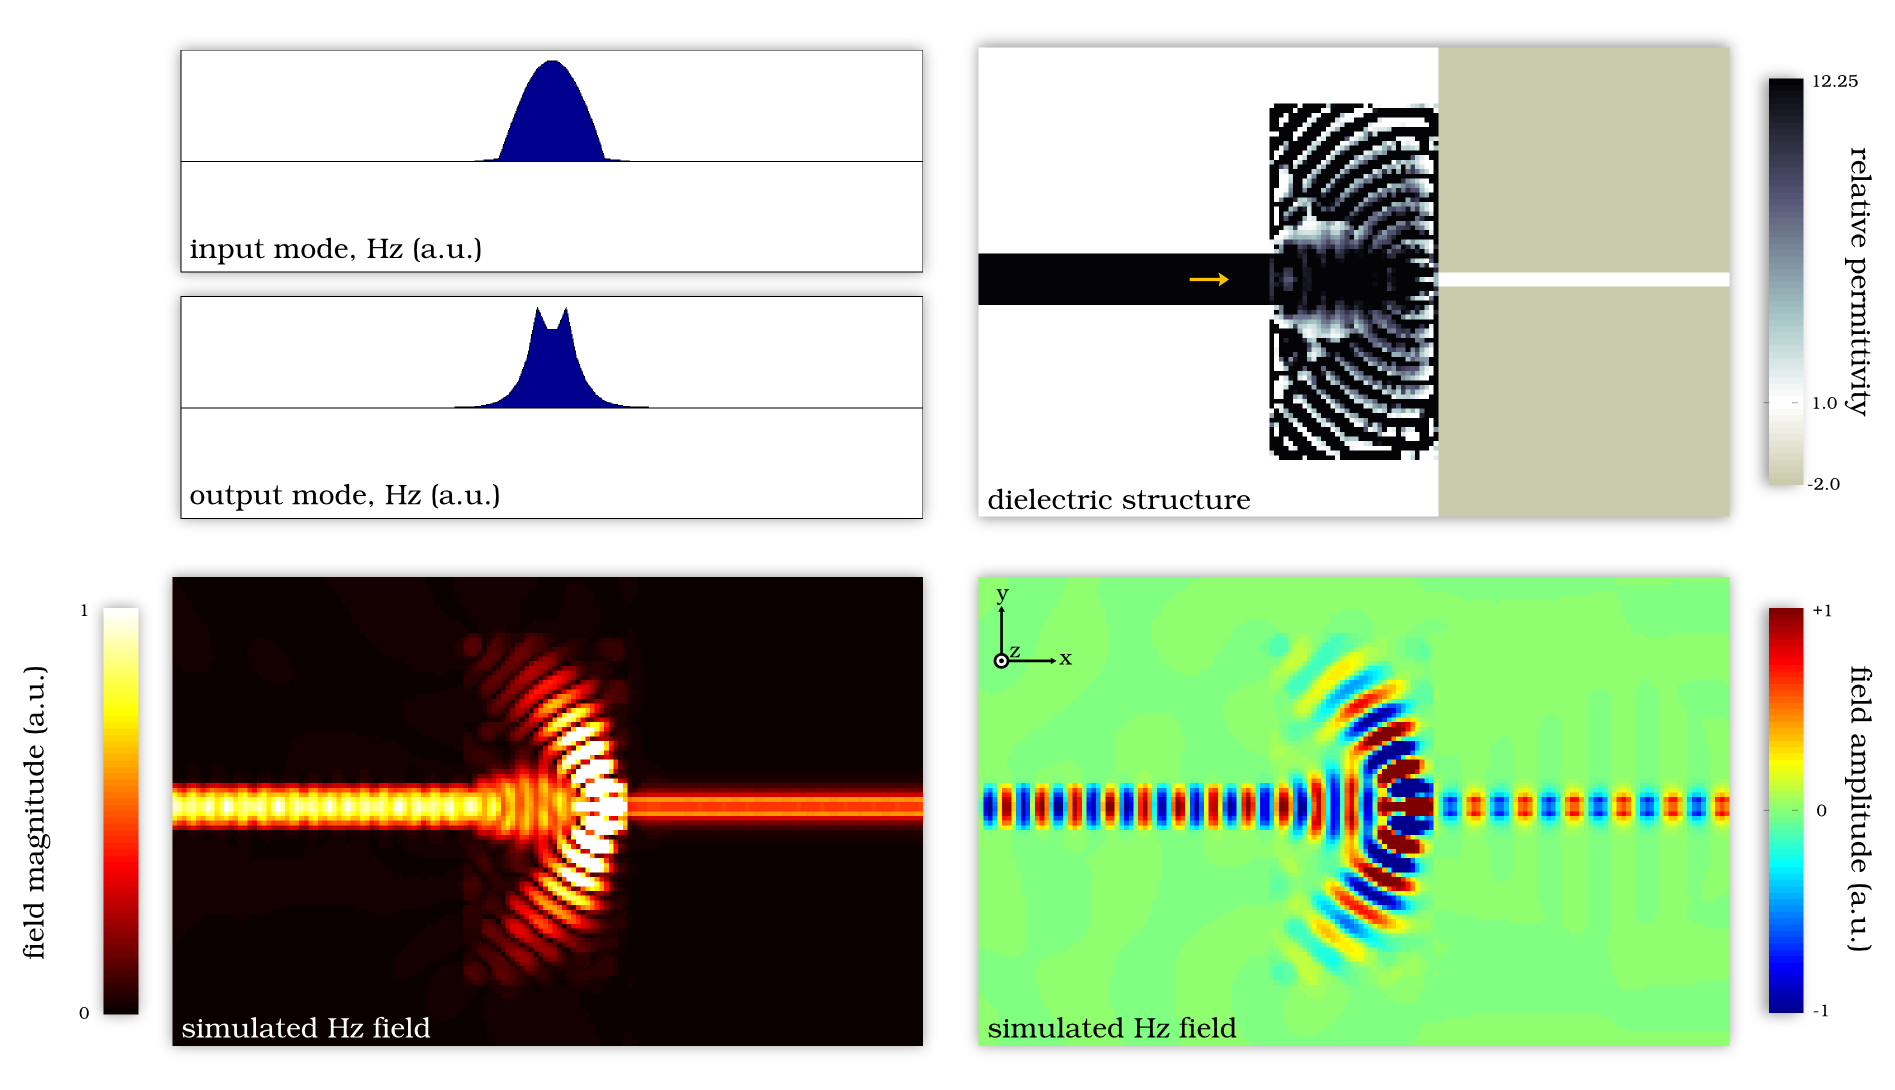
\includegraphics[width=\textwidth]{p3/4}
    \caption{Coupler between a dielectric slab waveguide to 
            a plasmonic metal-insulator-metal waveguide.
        The efficiency of the device is $97.5\%$ and 
            has the same wavelength and footprint as the device in
            Fig.~\ref{fig:aircore}.
        Computation time was 15 minutes on a personal computer.
        }
        \label{fig:mim}
\end{figure}
\begin{figure}[htb]
    \centering
    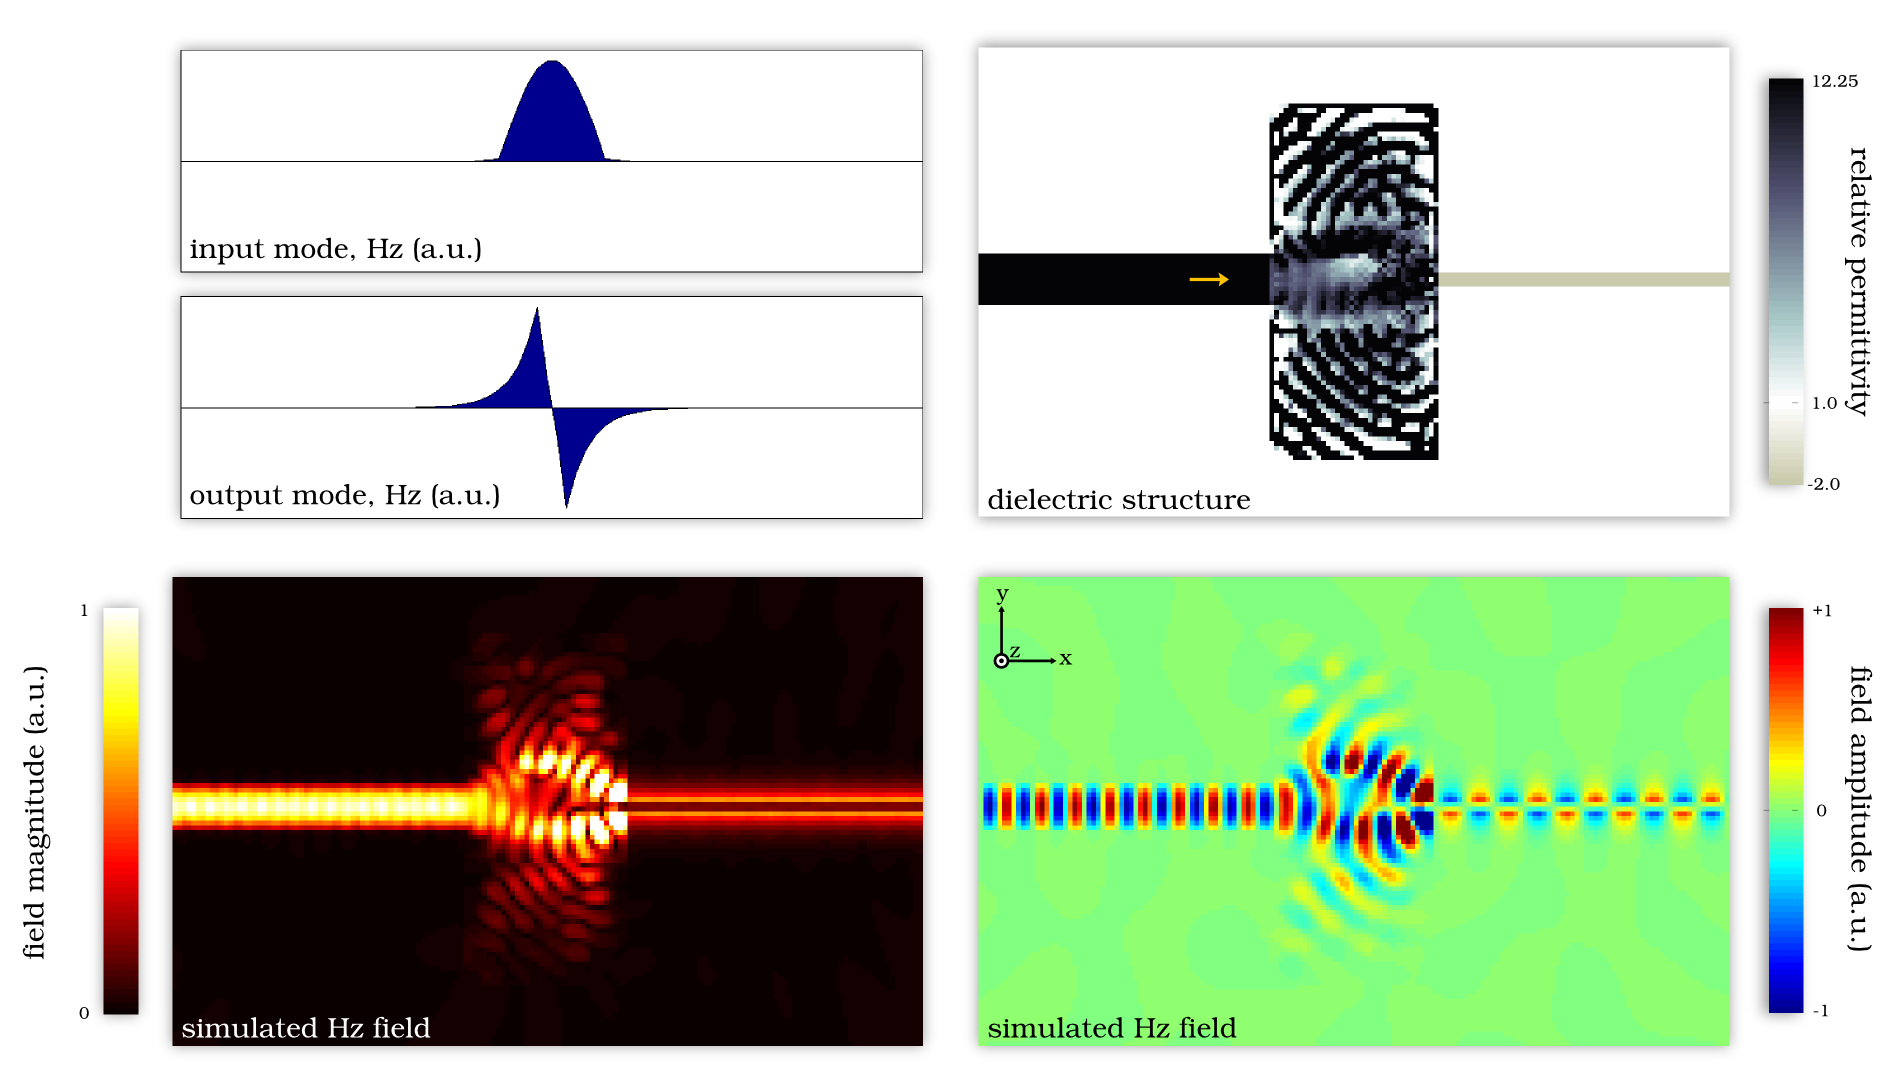
\includegraphics[width=\textwidth]{p3/5}
    \caption{Coupler between a dielectric slab waveguide to 
            a plasmonic wire waveguide.
        The efficiency of the device is $99.1\%$ and 
            has the same wavelength and footprint as the device in
            Fig.~\ref{fig:aircore}.
        Computation time was 15 minutes on a personal computer.
        }
        \label{fig:wire}
\end{figure}
% 
% \section{Conclusion}
% We develop a fundamentally new approach to designing physical structures,
%     which we term ``objective-first'', 
%     in that we choose to satisfy the design objective 
%     even above satisfying the physical equation which governs its operation.
% We then apply this approach to the design of 
%     various nanophotonic waveguide couplers,
%     and show that our method produces
%     high-efficiency designs ($\sim 98\%$ efficiency) 
%     in small footprints (1.5-4 square vacuum wavelengths)
%     without needing a good starting point.
% Furthermore, we suggest that such a methodology may be applicable
%     to the design of any single-mode, linear nanophotonic device.\\
% 
% This work has been supported by the 
%     AFOSR MURI for Complex and Robust On-chip Nanophotonics 
%     (Dr. Gernot Pomrenke), grant number FA9550-09-1-0704.
% The Matlab code used is available online\cite{code}.
% \clearpage
% \begin{appendix}


% % \documentclass[letterpaper,10pt]{article}
% \usepackage{graphicx}
% \usepackage{opex3}
% \usepackage{amsmath,amssymb}
% 
% 
% \newcommand{\myfig}[2]{
%     \begin{figure}[!h]
%     \begin{centering}
%     \includegraphics[width=0.8\textwidth]{fig/#1}
%     \caption{#2}\label{#1}
%     \end{centering}
%     \end{figure}
% }
% 
% \newcommand{\Eq}[1]{Eq.~\eqref{#1}}
% \newcommand{\Fig}[1]{Fig.~\ref{#1}}
% \newcommand{\eq}[1]{eq.~\eqref{#1}}
% \newcommand{\fig}[1]{fig.~\ref{#1}}
% \newcommand{\BI}{\begin{itemize}\item}
% \newcommand{\I}{\item}
% \newcommand{\EI}{\end{itemize}}
% \newcommand{\BEAS}{\begin{eqnarray}}
% \newcommand{\EEAS}{\end{eqnarray}}
% % \newcommand{\BEAS}{\begin{IEEEeqnarray}{rl}}
% % \newcommand{\EEAS}{\end{IEEEeqnarray}}
% \newcommand{\BSA}{\begin{subequations}\begin{align}}
% \newcommand{\ESA}{\end{align}\end{subequations}}
% \newcommand{\BE}{\begin{equation*}}
% \newcommand{\EE}{\end{equation*}}
% \newcommand{\BIT}{\begin{itemize}}
% \newcommand{\EIT}{\end{itemize}}
% 
% \newcommand{\eg}{{\it e.g.}}
% \newcommand{\ie}{{\it i.e.} }
% 
% \DeclareMathOperator*{\minimize}{\text{minimize}\quad}
% \newcommand{\subto}{\text{subject to}\quad}
% \newcommand{\T}{^\dagger}
% 
% 
% \newcommand{\ones}{\mathbf 1}
% \newcommand{\reals}{{\mbox{\bf R}}}
% \newcommand{\comps}{{\mbox{\bf C}}}
% \newcommand{\integers}{{\mbox{\bf Z}}}
% \newcommand{\symm}{{\mbox{\bf S}}}  % symmetric matrices
% 
% \newcommand{\nullspace}{{\mathcal N}}
% \newcommand{\range}{{\mathcal R}}
% \newcommand{\Rank}{\mathop{\bf Rank}}
% \newcommand{\Tr}{\mathop{\bf Tr}}
% \newcommand{\diag}{\mathop{\bf diag}}
% \newcommand{\lambdamax}{{\lambda_{\rm max}}}
% \newcommand{\lambdamin}{\lambda_{\rm min}}
% 
% \newcommand{\Expect}{\mathop{\bf E{}}}
% \newcommand{\Prob}{\mathop{\bf Prob}}
% \newcommand{\Co}{{\mathop {\bf Co}}} % convex hull
% \newcommand{\dist}{\mathop{\bf dist{}}}
% \newcommand{\argmin}{\mathop{\rm argmin}}
% \newcommand{\argmax}{\mathop{\rm argmax}}
% \newcommand{\epi}{\mathop{\bf epi}} % epigraph
% \newcommand{\Vol}{\mathop{\bf vol}}
% \newcommand{\dom}{\mathop{\bf dom}} % domain
% \newcommand{\intr}{\mathop{\bf int}}
% 
% \begin{document}
% 
% \title{Nanophotonic Computational Design}
% \author{Jesse Lu$^\ast$ and Jelena Vu\v{c}kovi\'{c}}
% \address{Stanford University, Stanford, California, USA.}
% \email{jesselu@stanford.edu}
% 
% \begin{abstract}
% In contrast to designing nanophotonic devices 
%     by tuning a handful of device parameters, 
%     we have developed a computational method 
%     which utilizes the full parameter space to design linear nanophotonic devices.
% We show that our method may indeed be capable of designing 
%     any linear nanophotonic device by demonstrating designed structures which
%     are fully three-dimensional and multi-modal,
%     exhibit novel functionality,
%     have very compact footprints,
%     exhibit high efficiency, and
%     are manufacturable.
% In addition, we also demonstrate the ability to produce structures
%     which are strongly robust to wavelength and temperature shift,
%     as well as fabrication error.
% Critically, we show that our method 
%     does not require the user to be a nanophotonic expert or 
%     to perform any manual tuning. 
% Instead, we are able to design devices 
%     solely based on the user's desired performance specification for the device.
% \end{abstract}
% \ocis{230.75370, 130.3990.}
% 
% \begin{thebibliography}{99}
% \bibitem{ob1_wg} J. Lu, J. Vuckovic, ``Objective-first design of high-efficiency, small-footprint couplers between arbitrary nanophotonic waveguide modes,'' 
%     Opt. Express \textbf{20}, 7221-7236 (2012)
% \bibitem{admm} S. Boyd, N. Parikh, E. Chu, B. Peleato, and J. Eckstein,
%     ``Distributed Optimization and Statistical Learning via the Alternating Direction Method of Multipliers,''
%     Foundations and Trends in Machine Learning \textbf{3}, 1-122 (2011). 
% \bibitem{wonseok} W. Shin and S. Fan, ``Choice of the perfectly matched layer boundary condition for frequency-domain Maxwell’s equations solvers,''
%     J. of Comp. Phys \textbf{231}, 3406-3431 (2012).
% \bibitem{levelset} S. Osher and R. Fedkiw, \emph{Level Set Methods and Dynamic Implicit Surfaces: 1st Edition} (Springer, 2002).
% \bibitem{2dsplitter} Y. Jiao, S. Fan, and D. A. B. Miller, 
%     ``Demonstrations of systematic photonic crystal design and optimization by low rank adjustment: an extremely compact mode separator'', Opt. Lett. \textbf{30}, 140-142 (2005).
% \bibitem{baets}F. Van Laere, G. Roelkens, M. Ayre, J. Schrauwen, D. Taillaert, D. Van Thourhout, T. F. Krauss, and R. Baets,
%     ``Compact and highly efficient grating couplers between optical fiber and nanophotonic waveguides,''
%     J. of Lightwave Tech. \textbf{25}, 151-156 (2007).
% % \bibitem{fibergrating} Y. Tang, Z. Wang, L. Wosinski, U. Westergren, and S. He,
% %     ``Highly efficient nonuniform grating coupler for silicon-on-insulator 
% %     nanophotonic circuits,''
% %     Opt. Lett. \textbf{35}, 1290-1292 (2010).
% % \bibitem{ridge}  K. K. Lee, D. R. Lim, L.C. Kimerling, J. Shin, and F. Cerrina, 
% %     ``Fabrication of ultralow-loss Si/SiO2 waveguides by roughness reduction,''
% %     Opt. Lett. \textbf{26}, 1888-1890 (2001).
% % \bibitem{pcslow} Y. A. Vlasov, M. O'Boyle, H. F. Hamann, and S. J. McNab,
% %     ``Active control of slow light on a chip with photonic crystal waveguides,''
% %     Nature \textbf{438}, 65-69 (2005).
% % \bibitem{slotfocus} M. Lipson, 
% %     ``Guiding, modulating, and emitting light on 
% %     silicon-challenges and opportunities,'' 
% %     J. Lightwave Technol. \textbf{23}, 4222-4238 (2005).
% % \bibitem{active} J. Van Campenhout, P. Rojo Romeo, P. Regreny, C. Seassal, 
% %     D. Van Thourhout, S. Verstuyft, L. Di Cioccio, J.-M. Fedeli, 
% %     C. Lagahe, and R. Baets, 
% %     ``Electrically pumped InP-based microdisk lasers integrated with a 
% %     nanophotonic silicon-on-insulator waveguide circuit,'' 
% %     Opt. Express \textbf{15}, 6744-6749 (2007).
% % \bibitem{metallic} L. Tang, S. E. Kocabas, S. Latif, A. K. Okyay, 
% %     D. S. Ly-Gagnon, K. C. Saraswat, and D. A. B. Miller, 
% %     ``Nanometre-scale germanium photodetector enhanced by a 
% %     near-infrared dipole antenna,'' 
% %     Nature Photonics \textbf{2}, 226-229 (2008).
% % % \bibitem{fwadia} V. R. Almeida, R. R. Panepucci, and M. Lipson, 
% % %     ``Nanotaper for compact mode conversion,'' 
% % %     Opt. Lett. \textbf{28}, 1302-1304 (2003) 
% % % \bibitem{wwadia} S. G. Johnson, P. Bienstman,  M. A. Skorobogatiy, 
% % %     M. Ibanescu1, E. Lidorikis, and J. D. Joannopoulos,
% % %     ``Adiabatic theorem and continuous coupled-mode theory for 
% % %     efficient taper transitions in photonic crystals,''
% % %     Phys. Rev. E \textbf{66}, 066608 (2002)
% % % \bibitem{deriv} F. Wang, J. S. Jensen, O. Sigmund, 
% % %     ``Robust topology optimization of photonic crystal waveguides with 
% % %     tailored dispersion properties.'' 
% % %     J. Opt. Soc. Am. B \textbf{28}, 387-397 (2011)
% % % \bibitem{boydbook} S. Boyd, and L. Vandenberghe, 
% % %     \emph{Convex Optimization} 
% % %     (Cambridge University Press, 2004)
% % \bibitem{prevwork} J. Lu, S. Boyd, and J. Vuckovic, 
% %     ``Inverse design of a three-dimensional nanophotonic resonator,''
% %     Opt. Express \textbf{19}, 10563-10750 (2011). 
% % \bibitem{veronis} G. Veronis, and S. Fan, 
% %     ``Theoretical investigations of compact couplers between dielectric slab 
% %     waveguides and two-dimensional metal-dielectric-metal plasmonic waveguides,'' 
% %     Opt. Express \textbf{15}, 1211-1221 (2007).
% % \bibitem{yang} R. Yang, R. A. Wahsheh, Z. Lu, and M. A. G. Abushagur, 
% %     ``Efficient light coupling between dielectric slot waveguide and plasmonic
% %     slot waveguide,'' Opt. Lett. \textbf{35}, 649-651 (2010).
% % \bibitem{code} \url{www.github.com/JesseLu/objective-first}
% \end{thebibliography}
\chapter{Nanophotonic computational design in 3D} \label{final}
% \section{Introduction}
% Currently, almost all nanophotonic components are designed 
%     by hand-tuning a small number of parameters 
%     (e.g. waveguide widths and gaps, hole and ring sizes).
% However, the realization of 
%     increasingly complex, dense, and robust on-chip optical networks
%     will require utilizing increasing numbers of parameters
%     when designing nanophotonic components.
% 
% Opening the design space to include many more parameters
%     allows for smaller footprint, higher performance devices by definition,
%     since original designs are still included in this parameter space.
% Unfortunately, the lack of intuition for what such designs might look like and
%     the inability to manually search such a large parameter space
%     have greatly hindered the ability to achieve this.
% 
% For this reason, we have developed and implemented a computational method
%     which is able to use the full parameter space 
%     to design linear nanophotonic components in three dimensions.
% Critically, our method requires no user intervention or manual tuning.
% Instead, a \emph{design-by-specification} scheme is used 
%     to produce designs based solely on a user's performance specification.
% 
% We show that our method can indeed produce designs 
%     which are extremely compact, and, at the same time, highly efficient.
% Furthermore, we demonstrate that devices with novel functionality
%     are easily designed.
% We also show that our method can be used to produce designs
%     with extreme robustness to wavelength and temperature shift,
%     as well as fabrication error.
% 
% Lastly, all our results are produced by simply specifying
%     the functionality and performance of the desired device,
%     which suggests that our method may indeed by able
%     to design \emph{all} linear nanophotonic devices.
% 
\section{Problem formulation}
In this central chapter of this work, 
    we present a method which may indeed be capable of designing 
    linear nanophotonic devices which
    are fully three-dimensional and multi-modal,
    exhibit novel functionality,
    have very compact footprints,
    exhibit high efficiency, and
    are manufacturable.
In addition, we also demonstrate the ability to produce structures
    which are strongly robust to wavelength and temperature shift,
    as well as fabrication error.

In order to produce designs which utilize the full parameter space,
    and are based solely on the user's performance specification,
    we use the following final formulation:
\begin{subequations}\begin{align}
    \minimize & \sum_i^M \|A_i(z)x_i - b_i\|^2 \\
    \subto & \alpha_{ij} \le |c_{ij}\T x_i| \le \beta_{ij}, \quad
        \text{for $i = 1, \ldots, M$ and $j = 1, \ldots, N_i$} \\
        &   z_\text{min} \le z \le z_\text{max}
\end{align} \label{problem}\end{subequations}

The explanation for the various terms in \eq{problem} follows:
\begin{enumerate}
\item 
    $A_i(z)x_i - b_i$ is the \emph{physics residual} for the $i$th mode.
    That is to say, $A_i(z)x_i - b_i$ represents the underlying physics
        of the problem; namely, the electromagnetic wave equation
        \mbox{$(\nabla\times\mu_0^{-1}\nabla\times - \omega_i^2 \epsilon) E_i 
            +i \omega_i J_i $}.

    The specific substitutions used in order to transform
        \BE (\nabla\times\mu_0^{-1}\nabla\times - \omega_i^2 \epsilon) E_i 
            +i \omega_i J_i  \quad\longrightarrow\quad A_i(z)x_i - b_i \EE
        are
    \BI $E_i \to x_i$,
    \I  $\epsilon \to z$,
    \I  $\nabla\times\mu_0^{-1}\nabla\times - \omega_i^2 \epsilon \to A_i(z)$, and
    \I  $ -i\omega_i J_i \to b_i$.  \EI

    In contrast to typical schemes for optimizing physical structures,
        our formulation actually allows for non-zero physics residuals;
        which can be deduced since $A_i(z)x_i-b_i=0$ is not a hard constraint.
    Instead, this formulation is what also an \emph{objective-first} \cite{Lu12}
        formulation in that the \emph{design objective} (explained below)
        is prioritized above satisfying physics.

\item
    The (field) design objective consist of 
        the constraint $\alpha_{ij} \le |c_{ij}\T x_i| \le \beta_{ij}$.
    Physically, this constraint describes 
        the performance specification of the device 
        via a series of field overlap integrals 
        at various output ports of the device.
    Specifically, the $c_{ij}\T x_i$ terms represents an overlap integral between
        the E-field of the $i$th mode ($x_i$)
        with an E-field of the user's choice ($c_{ij}$),
        where the additional subscript $j$ allows the user
        to include multiple such fields.
    The amplitude of the overlap integral is then forced to reside between
        $\alpha_{ij}$ and $\beta_{ij}$.

    This mechanism allows the user to express 
        the desired performance of the device
        as a combination of field amplitudes in various output field patterns.
    These outputs would be in response to a predefined input excitation,
        which is determined by the current excitation $b_i$ ($-i\omega_i J_i$)
        in the physics residual of each mode.

    As an example of a design objective for some mode 1 
        a user might choose to have the majority of the output power
        reside in some output pattern 1,
        while ensuring that only a small amount of power 
        be transferred to some output pattern 2.
    In this case the user would use 
        $0.9 \le |c_{11}\T x_1| \le 1.0$ for the former.
        and then $0.0 \le |c_{12}\T x_1| \le 0.01$ for the latter;
        where $c_{11}$ and $c_{12}$ are representative of 
        output patterns 1 and 2 respectively.

    We note that although the performance description of nearly all
        linear devices can be specified using such a constraint,
        the constraint itself is \emph{not} linear (neither is it convex).
    Other performance objectives are indeed possible which are nonlinear 
        and nonconvex (such as optimizing for energy density or Q-factor)---convex 
        objectives would be straightforward to implement,
        while some non-convex objectives would require clever heurestics.
        
    Finally, we note again that the design objective in our formulation
        is actually a hard constraint.
    This means that it is \emph{always satisfied}, 
        even to the extent of allowing for an unphysical field 
        (since the physics residual will not be exactly 0).
    It is for this reason that we call such a formulation ``objective-first''.

\item 
    The final term in \eq{problem}, $z_\text{min} \le z \le z_\text{max}$,
        is the structure design objective.
    It is used as a relaxation of the binary constraint,
        $z \in \{z_\text{min}, z_\text{max}\}$,
        which would ensure that the final design be composed 
        of two discrete materials.
\end{enumerate}

\section{Implementation}
We employed the alternating directions method of multipliers (ADMM) algorithm 
    \cite{Boyd11}
    in order to solve \eq{problem}.
The ADMM algorithm solves \eq{problem} by iteratively solving for 
    $x_i$, $z$, and a dual variable $u_i$.

Since we are working in three dimensions, solving \eq{problem} for $x_i$ 
    is non-trivial in that it involves millions of variables and
    requires solving for the ill-conditioned $A_i(z)$ matrix.
For this reason, we use a home-built
    finite-difference frequency-domain (FDFD) solver which 
    implements a hardware-accelerated iterative solver\cite{Shin12}
    on Amazon's Elastic Compute Cloud.
Critically, our cloud-based solver allows us to scale to solve problems
    with arbitrarily-large number of modes,
    with no significant penalty in runtime.

In contrast to solving for $x_i$, solving for $z$ is much simpler since we
    only consider planar structures;
    thereby limiting $z$ to have only thousands of variables.

Lastly, in order to arrive at fully discrete, manufacturable structures,
    we convert $z$ to a boundary parameterization\cite{Osher02}
    and tune our structure using a steepest-descent method.

The mathematical details of our implementation are given 
    in appendix~\ref{maths}

\section{Results}
We demonstrate the effectiveness of our design method 
    by producing designs for a variety of nanophotonic devices\cite{Lu13}.

\emph{All of our results are in three dimensions
    and are planar structures, consisting of a 250 nm etched silicon slab
    completely surrounded by silica.}
The permittivity values of silicon and silica used
    were $\epsilon_\text{Si} = 12.25$ and $\epsilon_\text{SiO$_2$} = 2.25$
    respectively.

Many, if not all, of the produced designs exhibit 
    novel functionality, high efficiency, and 
    very compact footprints of only a few square vacuum wavelengths,
    while still remaining manufacturable.
We also show that many devices can be designed
    to exhibit different functionality for different input excitations.
Additionally, we show that devices can be designed with large tolerances for
    errors in wavelength, temperature and fabrication.

% Runtimes for the design process ranged from 8-80 hours 
%     based on the size of the design space.
\subsection{Mode converters}

Our first devices consisted of waveguide mode converters.
Such devices are simple in that they are single-input, single-output devices.
At the same time, such a device is significant because 
    it demonstrates the feasibility of multi-mode on-chip optical networks
    by showing that high-efficiency mode conversion 
    can readily be achieved in planar on-chip nanophotonic structures.

We show, through the design of mode converters for both the TE- and TM-polarized
    waveguide modes, 
    that our method is indeed fully three-dimensional.
Additionally, the devices also demonstrate very small device footprints 
    ($1.6 \times 2.4$ microns for this device in particular
    operating at 1550 nm wavelength).

\subsubsection{TE mode converter}
Our first result is a mode conversion device operating in the TE polarization,
    where the primary E-field component
    of the waveguide mode is polarized in the plane of the structure.

Our performance specification (\fig{3Db_wgc_te2}) 
    for the device was for $\ge90\%$ of the 
    input power to be transferred from the fundamental waveguide mode,
    to the second-order waveguide mode.
At the same time, we specified that no more than 1\% of the input power
    was to remain in the transmitted fundamental mode.

\myfig{3Db_wgc_te2}
    {Perfomance specification of the TE mode converter.
    Input mode is the fundamental TE-polarized mode on the top-left.
    Primary output mode is the second-order mode on the top-right.
    Output power in the transmitted fundamental mode (bottom-right) 
    should be no more than 1\%.
    The structure shown is the final three-dimensional design
    (the same holds for all the following figures in the article).
%     The x- and y-axes are in the plane of the structure,
%         with the x-axis is the direction of propagation 
%         for the input and output waveguides.
%     As expected, the z-axis is perpendicular to the plane of the structure.
    }

The performance of the device is shown in \fig{takeaway}.
The conversion efficiency into the second-order mode is lower
    than desired (86.4\%). 
Imperfect conversion may be due to evanescent modes ``interfering'' 
    with the output field overlap calculation.

\myfig{takeaway}
    {Structure and E-field at the central plane of the TE mode converter.
    The conversion efficiency into the second-order mode is 86.4\%,
    while the power into the rejection mode (fundamental) is 0.7\%.
    Device footprint is $1.6\times2.4$ microns.
    Operating wavelength is 1550 nm.}


\subsubsection{TM mode converter}

In addition to mode conversion in the TE polarization (E-field in-plane),
    we show that TM polarization (E-field out-of-plane) mode converters
    can be designed as well.
This example shows that full three-dimensional structures 
    truly are possible,
    and that no approximations are needed for our method.

Since our method is design-by-specification, 
    the design of a TM mode converter requires only
    a small modification to the performance specification of the device;
    namely the polarization of the input and output modes (\fig{3Db_wgc_tm}).
Specifically, we still design for 
    $\ge 90\%$ conversion into the second-order mode and 
    a $\le 1\%$ allowance for the fundamental mode to be transmitted.

\myfig{3Db_wgc_tm}
    {Perfomance specification of the TM mode converter.
    Input mode is the fundamental TM-polarized mode on the top-left.
    Primary output mode is the second-order mode on the top-right.
    Output power in the transmitted fundamental mode on the bottom-right 
    should be under 1\%.
    The structure shown is the final three-dimensional design.}
    
The performance of the device is shown in \fig{wgc_tm}.
The lower conversion efficiency of 76.9\% in contrast to the TE mode converter
    may be attributed to the lower confinement of the TM waveguide modes 
    in such thin slabs.
However, good rejection of only 1\% is still achieved.

\myfig{wgc_tm}
    {Structure and E-field at the central plane of the TM mode converter.
    The conversion efficiency into the second-order mode is 76.9\%,
    while the power into the rejection mode (fundamental) is 1.0\%.
    Device footprint is $1.6\times2.4$ microns.}

\subsection{Mode splitters}
Next, we demonstrate the design of nanophotonic waveguide mode splitters.
Such devices can be used as multiplexers or demultiplexers and
    are the key component in utilizing a single waveguide to transmit 
    multiple optical signals.

As a demonstration of the versatility of our method, 
    we show that it is capable of designing mode splitting devices 
    based on either the spatial profile, the polarization, or the wavelength
    of the input modes.

The performance specification for each device is simply to convert
    more than 90\% of the input power in a particular input mode into
    either one of the output modes.
At the same time, we specify that the transmission into the other output mode 
    be kept below 1\% of input power.

\subsubsection{Spatial mode splitter}
We demonstrate what is, to our knowledge, 
    the first design for a three-dimensional
    nanophotonic spatial mode splitter 
    (previous designs were restricted to two dimensions \cite{Jiao05}).
Such a device is the key enabler for multi-mode on-chip optical circuits,
    and we show here that they can be designed to be highly efficient
    while utilizing a very small device footprint ($2.8\times2.8$ microns). 
The performance specification is shown in \fig{3Db_spl_modal},
    and the final results is shown in \fig{spl_modal}.

\myfig{3Db_spl_modal}
    {Spatial mode splitter performance specification.
    Input mode is either the fundamental or second-order
        TE-polarized mode on the left.
    Output modes are the fundamental waveguide modes of either output 
        waveguide on the right.
    Output power into the desired output arm is specified to be greater than 90\%,
        while power into the opposing arm is set to below 1\%.}
\myfig{spl_modal}
    {Spatial mode splitter final result.
    The conversion efficiencies into the upper and lower output arms
        are 88.7\% and 77.4\% respectively, 
        while the rejection powers for the same modes are 0.27\% and 0.20\%.
    Device footprint is $2.8\times2.8$ microns.}

\subsubsection{TE/TM splitter}
In addition to splitting different spatial modes, 
    we show that different polarizations can also be split.
\Fig{3Db_spl_tetm} shows the performance specification of a 
    device which is able to separate fundamental TE-polarized ($E_y$ dominant)
    and TM-polarized ($E_z$ dominant)
    waveguide modes into separate arms.
The final, verified result is shown in \fig{spl_tetm}.

Not only is this result the first of its kind,
    it is the first in the device category where a single device
    is able to control both polarizations within the same device footprint.
This shows the versatility and broad applicability of our method.

\myfig{3Db_spl_tetm}
    {TE/TM splitter performance specification.
    Input mode is either the fundamental TE-polarized ($E_y$ dominant, top left)
    and TM-polarized ($E_z$ dominant, top right).
    Output power into the desired output arm is specified to be greater than 90\%,
        while power into the opposing arm is set to below 1\%.}
\myfig{spl_tetm}
    {TE/TM splitter final result.
    The conversion efficiencies into the upper and lower output arms
        are 87.6\% and 88.8\% respectively, 
        while the rejection powers for the same modes are 1.06\% and 0.58\%.
    Device footprint is $2.8\times2.8$ microns.}

\subsubsection{Wavelength splitter}
Traditional wavelength splitting devices can also be designed using our method.
Here, we show that the 1550 nm and 1310 nm wavelengths can be split
    in a very small device footprint ($2.8\times2.8$ microns).
The performance specification is shown in \fig{3Db_spl_wdm}, 
    and the final result is shown in \fig{spl_wdm}.
\myfig{3Db_spl_wdm}
    {Wavelength splitter performance specification.
    Input mode is the fundamental TE-polarized mode on the left at 
        a wavelength of either 1550 nm or 1330 nm.
    Output modes are the fundamental waveguide modes of either output 
        waveguide on the right;
        however, the 1550 nm wavelength is directed into the top output, 
        while the 1310 nm wavelength is directed into the bottom output.
    Output power into the desired output arm is specified to be greater than 90\%,
        while power into the opposing arm is set to below 1\%.}
\myfig{spl_wdm}
    {Wavelength splitter final result.
    The conversion efficiencies into the upper and lower output arms
        are 83.2\% and 78.7\% respectively, 
        while the rejection powers for the same modes are 0.49\% and 1.66\%.
    Device footprint is $2.8\times2.8$ microns.}

\subsection{Hubs}
We continue to demonstrate the capabilities of our method
    by designing multi-input, multi-output devices which we call \emph{hubs}.
Such devices essentially re-arrange modes in the waveguides,
    and may be thought of as general cross-connect structures.
Critically, the successful design of such structures 
    shows that efficiently routing overlapping signals can be 
    accomplished in a single layer for nanophotonic circuits.

\subsubsection{3$\times$3 hub}
We first design a hub with three inputs and outputs.
The performance specification is shown in \fig{3Db_hub_3x3},
    and the final result is shown in \fig{hub_3x3}.

\myfig{3Db_hub_3x3}
    {3$\times$3 hub performance specification.
    Input and output modes all consist of the fundamental TE-polarized mode.
    Output power into the desired output arm is specified to be greater than 90\%,
        no rejection modes are used for computational efficiency.
    This hub directs input power from input ports 1, 2, and 3 (from top to bottom)
    into output ports 2, 3, and 1 respectively.}
\myfig{hub_3x3}
    {3$\times$3 hub final result.
    The conversion efficiencies into the selected output arms
        are 88.6\%, 90.6\%, and 87.3\% for 
        input arms 1, 2, and 3 respectively (top to bottom).}

\subsubsection{4$\times$4 hub}
We extend our previous result to design a hub with four inputs and outputs.
The performance specification is shown in \fig{3Db_hub_4x4},
    and the final result is shown in \fig{hub_4x4_comb}.

\myfig{3Db_hub_4x4}
    {4$\times$4 hub performance specification.
    Input and output modes all consist of the fundamental TE-polarized mode.
    Output power into the desired output arm is specified to be greater than 90\%,
        no rejection modes are used for computational efficiency.
    This hub directs input power from input ports 1, 2, 3, and 4
    into output ports 3, 2, 4, and 1 respectively.}
\myfig{hub_4x4_comb}
    {4$\times$4 hub final result.
    The conversion efficiencies into the selected output arms
        are 85.9\%, 88.1\%, 85.4\%, and 84.3\% for
        input arms 1, 2, 3, and 4 respectively (top to bottom).}
\clearpage

\subsubsection{2$\times$2$\times$2 hub}
We can now design a hub that performs 
    different switching functions for different wavelengths.
Specifically, we use two input waveguides, two output waveguides,
    and two wavelengths (hence the name 2$\times$2$\times$2).

Our performance specification (\fig{3Db_hub_2x2x2}) is
    to cross-couple the waveguides at the 1310 nm wavelength,
    but to uncouple the waveguides at the 1550 nm wavelength.
The final result is shown in \fig{hub_2x2x2}.
\myfig{3Db_hub_2x2x2}
    {2$\times$2$\times$2 hub performance specification.
    Input and output modes all consist of the fundamental TE-polarized mode
        at either 1550 nm or 1310 nm wavelengths.
    Output power into the desired output arm is specified to be greater than 80\%,
        no rejection modes are used for computational efficiency.
    This hub directs input arms 1 and 2 into output arms 1 and 2 at 1550 nm,
        but swaps them at 1310 nm.}
\myfig{hub_2x2x2}
    {2$\times$2$\times$2 hub final result.
    The conversion efficiencies at the 1550 nm wavelength 
        are 77.6\% and 73.7\% respectively for the top and bottom inputs.
    At 1310 nm, the respective efficiencies are 75.7\% and 75.2\%.}
\clearpage 

\subsection{Fiber couplers}
The capabilities of our method are further demonstrated
    in the design of nanophotonic fiber couplers,
    which couple light from an optical fiber at normal incidence
    into an in-plane waveguide\cite{Laere07}.

The structure of the optical fibers used was a 2 micron diameter core with 
    refractive index $n_\text{core} = 1.6$,
    surrounded by a cladding with refractive index $n_\text{cladding}=1.5$.
The reduced size of the fiber core was employed in order
    to keep the device footprint small.
Additionally, the fiber coupler devices were only etched to half the membrane depth,
    in order to increase the asymmetry in the device structure.

\subsubsection{Compact fiber coupler}
We first present the design of a compact fiber coupler.
Such a device is said to be compact in that the functions
    of coupling into the plane, and focusing into a narrow waveguide
    are overlapped in the same device footprint.

Although the performance specification (\fig{3Db_fib_te})
    desired a coupling efficiency above 90\%,
    only 51.5\% efficiency was achieved (\fig{fib_te}).

\myfig{3Db_fib_te}
    {Compact fiber coupler performance specification.
    Input mode consists of the $E_y$-polarized fundamental fiber mode.
    Output mode is the fundamental TE-polarized mode of the in-plane waveguide.
    Output power into the desired output arm is specified to be greater than 90\%.}
\myfig{fib_te}
    {Compact fiber coupler final result.
    The conversion efficiency into the in-plane waveguide mode is 51.5\%.}

\subsubsection{Mode-splitting fiber coupler}
We now continue to show how different functionalities
    can be incorporated into a single device,
    by virtue of our design-by-specification scheme.

Here, we show how the functionality of a fiber coupler
    can be combined with that of a spatial mode splitter.
Specifically, the performance specification (\fig{3Db_fib_pol})
    determines that different fiber spatial modes
    by split into different in-plane nanophotonic waveguides.

The final result (\fig{fib_pol}) has lower efficiencies;
    however, the result is still useful 
    in that no device with such a functionality has previously been demonstrated.

\myfig{3Db_fib_pol}
    {Mode-splitting fiber coupler performance specification.
    Input mode consists of the fundamental fiber mode or 
        the third-order, circularly polarized fiber mode.
    Output mode is the fundamental TE-polarized mode of either in-plane waveguide.
    The device is designed to couple the fundamental fiber mode into
        the upper output arm, 
        while the third-order fiber mode is coupled into the lower output arm.
    Output power into the desired output arm is specified to be greater than 90\%.}
\myfig{fib_pol}
    {Mode-splitting fiber coupler final result.
    The conversion efficiency for the fundamental fiber mode input is 32.6\% 
        (top plot).
    The conversion efficiency for the third-order fiber mode input is 22.7\% 
        (bottom plot).}

\subsubsection{Wavelength-splitting fiber coupler}
Another example of a functionality-combining device is the wavelength-splitting
    fiber coupler.
Here, fiber modes of different wavelengths are coupled in-plane
    and then split into different nanophotonic waveguides (\fig{3Db_fib_wdm}).
Once again, efficiencies are low (\fig{fib_wdm}),
    but no such device has previously been demonstrated.

\myfig{3Db_fib_wdm}
    {Wavelength-splitting fiber coupler performance specification.
    Input mode consists of the $E_y$-polarized fundamental fiber mode at either
        the 1310 nm or 1550 nm wavelengths.
    Output mode is the fundamental TE-polarized mode of either in-plane waveguide.
    The structure is designed to guide light at the 1550 nm wavelength
        into the upper output arm,
        while 1310 nm light is guided into the lower output arm.
    Output power into the desired output arm is specified to be greater than 90\%.}
\myfig{fib_wdm}
    {Wavelength-splitting fiber coupler final result.
    The conversion efficiency into the in-plane waveguide mode at 1550 nm is 31.6\%.
    The conversion efficiency into the in-plane waveguide mode at 1310 nm is 28.6\%.}

\subsection{Broadband wavelength splitter}
We continue to investigate the capabilites of our method
    by attempting the design of a broadband wavelength splitter.

First, we revisit our wavelength splitter result (\fig{spl_wdm})
    and perform a broadband analysis, 
    the results of which are shown in \fig{analysis_spl_only}.
This analysis reveals that device performance quickly drops off
    as one moves away from the target wavelengths.
\myfig{analysis_spl_only}
    {Broadband analysis of previously design wavelength splitter (\fig{spl_wdm}).
    Although high-efficiency operation is achieved, 
    the performance quickly drops off away from the target wavelengths 
    (denoted by arrows).}

In order to design a broadband wavelength splitter,
    we modify our performance specification to include multiple target 
    wavelengths (with identical desired performance) around the 
    original target wavelengths, as seen in \fig{analysis_top}
    which reveals that broadband operation has been achieved.
The final result for the broadband wavelength splitter is shown in \fig{top_wdm}.
\myfig{analysis_top}
    {Broadband analysis of broadband wavelength splitter 
        (final design shown in \fig{top_wdm}.
    The addition of multiple target wavelengths (vertical arrows)
    allows for 
    high-efficiency operation is achieved across a wide bandwidth.}
\myfig{top_wdm}
    {Broadband wavelength splitter final result.
    The efficiencies at the central target wavelengths of 1550 nm and 1310 nm
    exceed those of its narrowband counterpart (\fig{spl_wdm}).}

\subsubsection{Temperature-robustness of broadband wavelength splitter}
We can now perform a temperature analysis of our broadband wavelength splitter,
    using $\Delta n_\text{Si} / \Delta T = 1.85 \cdot 10^{-4} K^{-1}$ 
    and $\Delta n_{\text{SiO}_2} / \Delta T = 0$ 
    (no refractive index shift for silica).
This analysis, shown in \fig{analysis_temp_shift2},
    reveals that stable operating points exist
    over a temperature range of nearly 1000 K.
Such a result is telling in that it demonstrates
    that on-chip optical devices can be designed to be \emph{passively} stable
    to temperature shifts which would typically be present in CPUs,
    since these are much less than 1000 K.
\myfig{analysis_temp_shift2}
    {Temperature analysis of the broadband wavelength splitter.
    Stable operating points (defined as efficiency $\ge$ 80\%)
    exist over a temperature shift of 905K.}

\subsubsection{Fabrication-robustness of broadband wavelength splitter}
A analysis with regard to fabrication-error
    was also performed on the broadband wavelength splitter.
The specific fabrication error was a general over- or under-etch
    of the device (input and output waveguides unaffected)\cite{robust1}.
\Fig{analysis_fab_shift2} reveals that up to 8 nm of over- or under-etching
    can be sustained before performance falls below 70\%, at the central
    operating wavelengths.
The structural variations at 8 nm of etch error are shown in \fig{top_wdm_overunder}.
    
\myfig{analysis_fab_shift2}
    {Analysis of fabrication-error on the performance of the broadband 
    wavelength splitter.
    Original central wavelengths are shown to hold greater than 70\% efficiency,
    in spite of up to 8 nm of over- or under-etch error.}
\myfig{top_wdm_overunder}
    {Comparison of under-etched, as-designed, and over-etched structures.
    Differences are subtle since the pixel size is 40 nm and the
    fabrication error is 8 nm.}

This result is significant in that it demonstrates
    that the design of broadband devices
    seems to be a valid heuristic in the search for 
    devices which are tolerant to temperature shifts and fabrication error.
Note, however, that our method, as formulated, is also able to
    deal with temperature and fabrication shifts explicitly as well,
    although such results are not demonstrated here.

% \section{Conclusion}
% We have developed and implemented a method to design linear nanophotonic structures
%     which are fully three-dimensional and multi-modal,
%     have very compact footprints,
%     exhibit high efficiency, and
%     are manufacturable.
% We demonstrate this capability by designing various nanophotonic mode converters,
%     splitters, hubs, and fiber couplers.
% Critically, many, if not all, of these devices have never been demonstrated before
%     and cannot be designed by hand.
% In contrast, our method allows user to easily design such devices
%     by virtue of our design-by-specification scheme.
% 
% In addition, we demonstrate the design of a broadband device 
%     which is strongly robust to wavelength and temperature shift,
%     as well as fabrication error.
% We show that such a device has stable operating wavelengths 
%     over temperature shifts as large as 905 K,
%     or over-/under-etching error of up to 8 nm.
% We suggest, based on this design, that wavelength tolerance
%     may be a good heuristic to the design of temperature and fabrication-error
%     tolerant nanophotonic devices. \\
% 
% \end{document}

% \include{chapter5}

% and the end material

% \appendix
% 
% \chapter{Additional objective-first results}\label{ob-1 additional}
\section{Additional mode coupler designs}
In this section, we present additional mode coupler designs based 
    on the objective-first strategy outlined in chapter~\ref{ob-1}.
A wide, high-index waveguide is used at both the input and output ports,
    and all permutations of couplers are fabricated among
    the first four propagating modes.
\begin{figure}[h!]
    \centering
    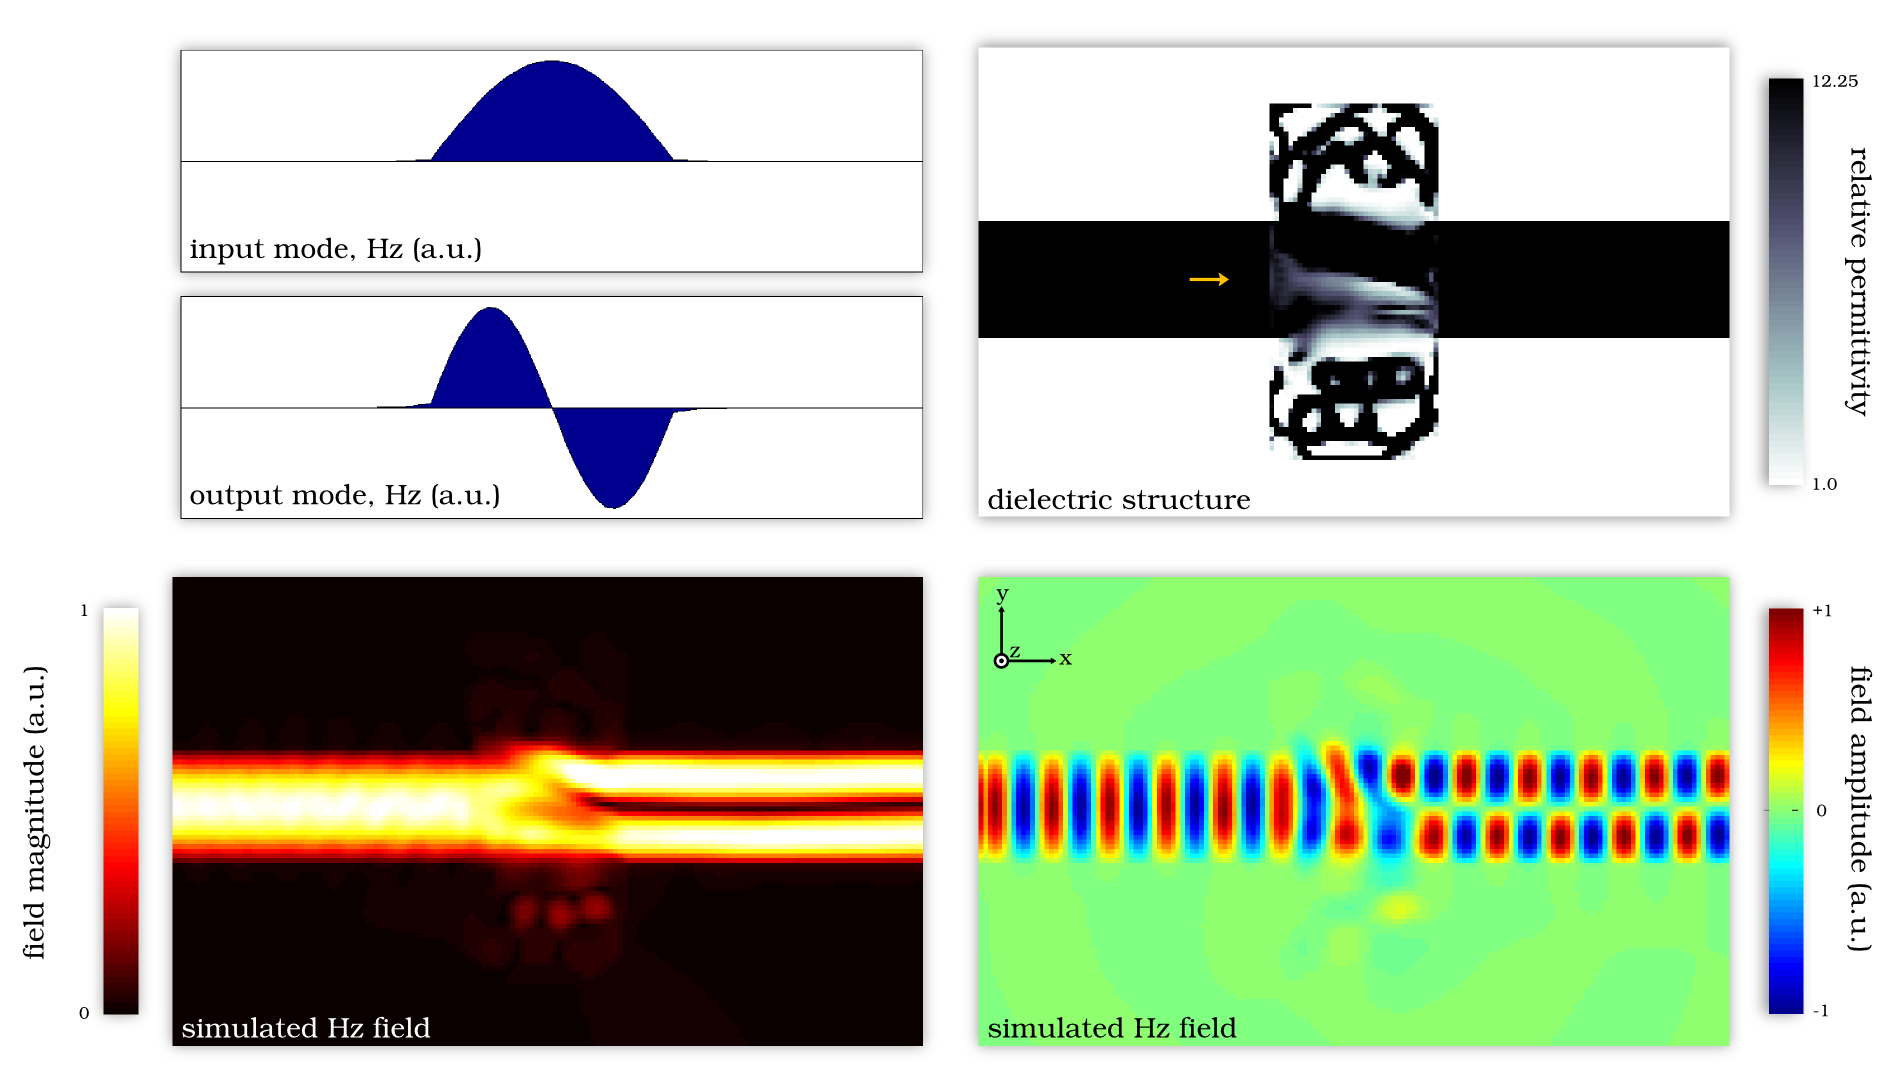
\includegraphics[width=\textwidth]{p3/6}
    \caption{
        Coupler from the first-order to the second-order mode 
            of a wide dielectric waveguide.
        Efficiency: $99.3\%$,
        footprint: $1.55$ square vacuum wavelengths.
        }
        % \label{fig:wire}
\end{figure}
\begin{figure}[h!]
    \centering
    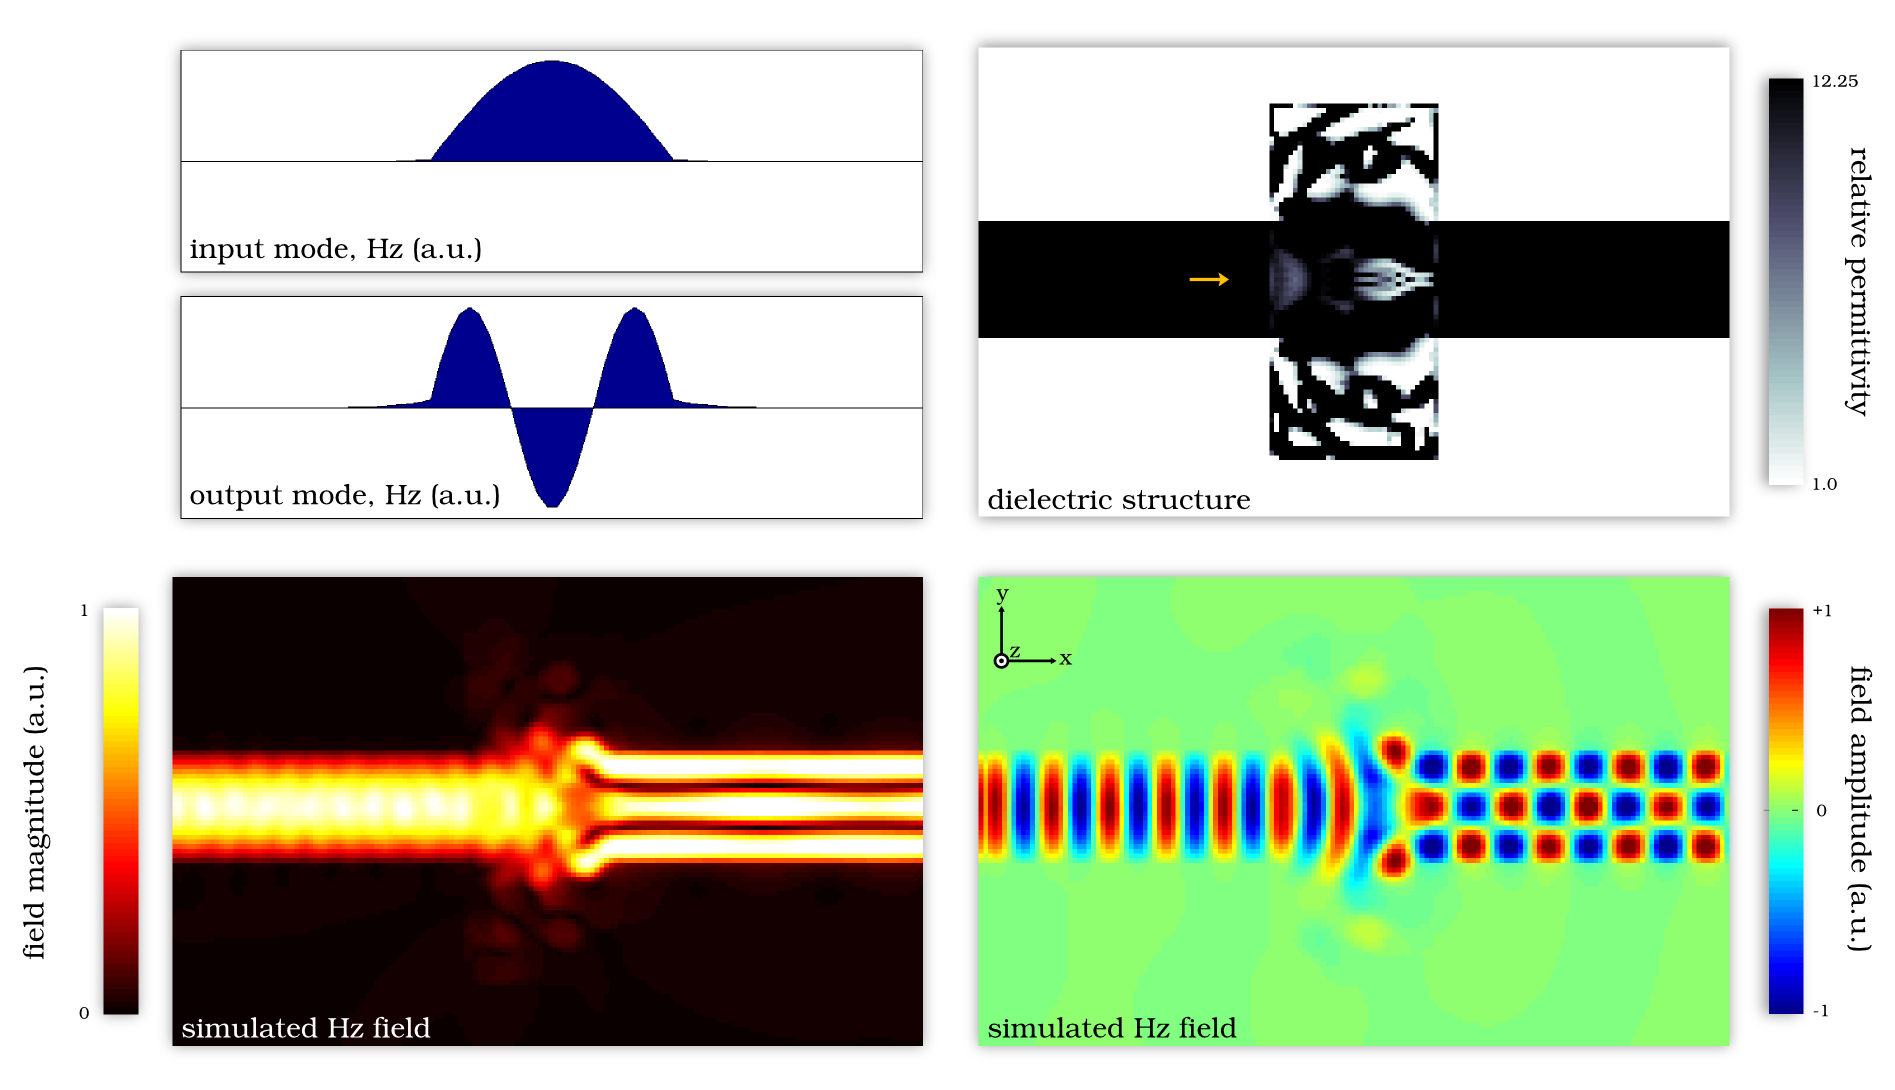
\includegraphics[width=\textwidth]{p3/7}
    \caption{
        Coupler from the first-order to the third-order mode 
            of a wide dielectric waveguide.
        Efficiency: $98.3\%$,
        footprint: $1.55$ square vacuum wavelengths.
        }
        % \label{fig:wire}
\end{figure}
\begin{figure}[h!]
    \centering
    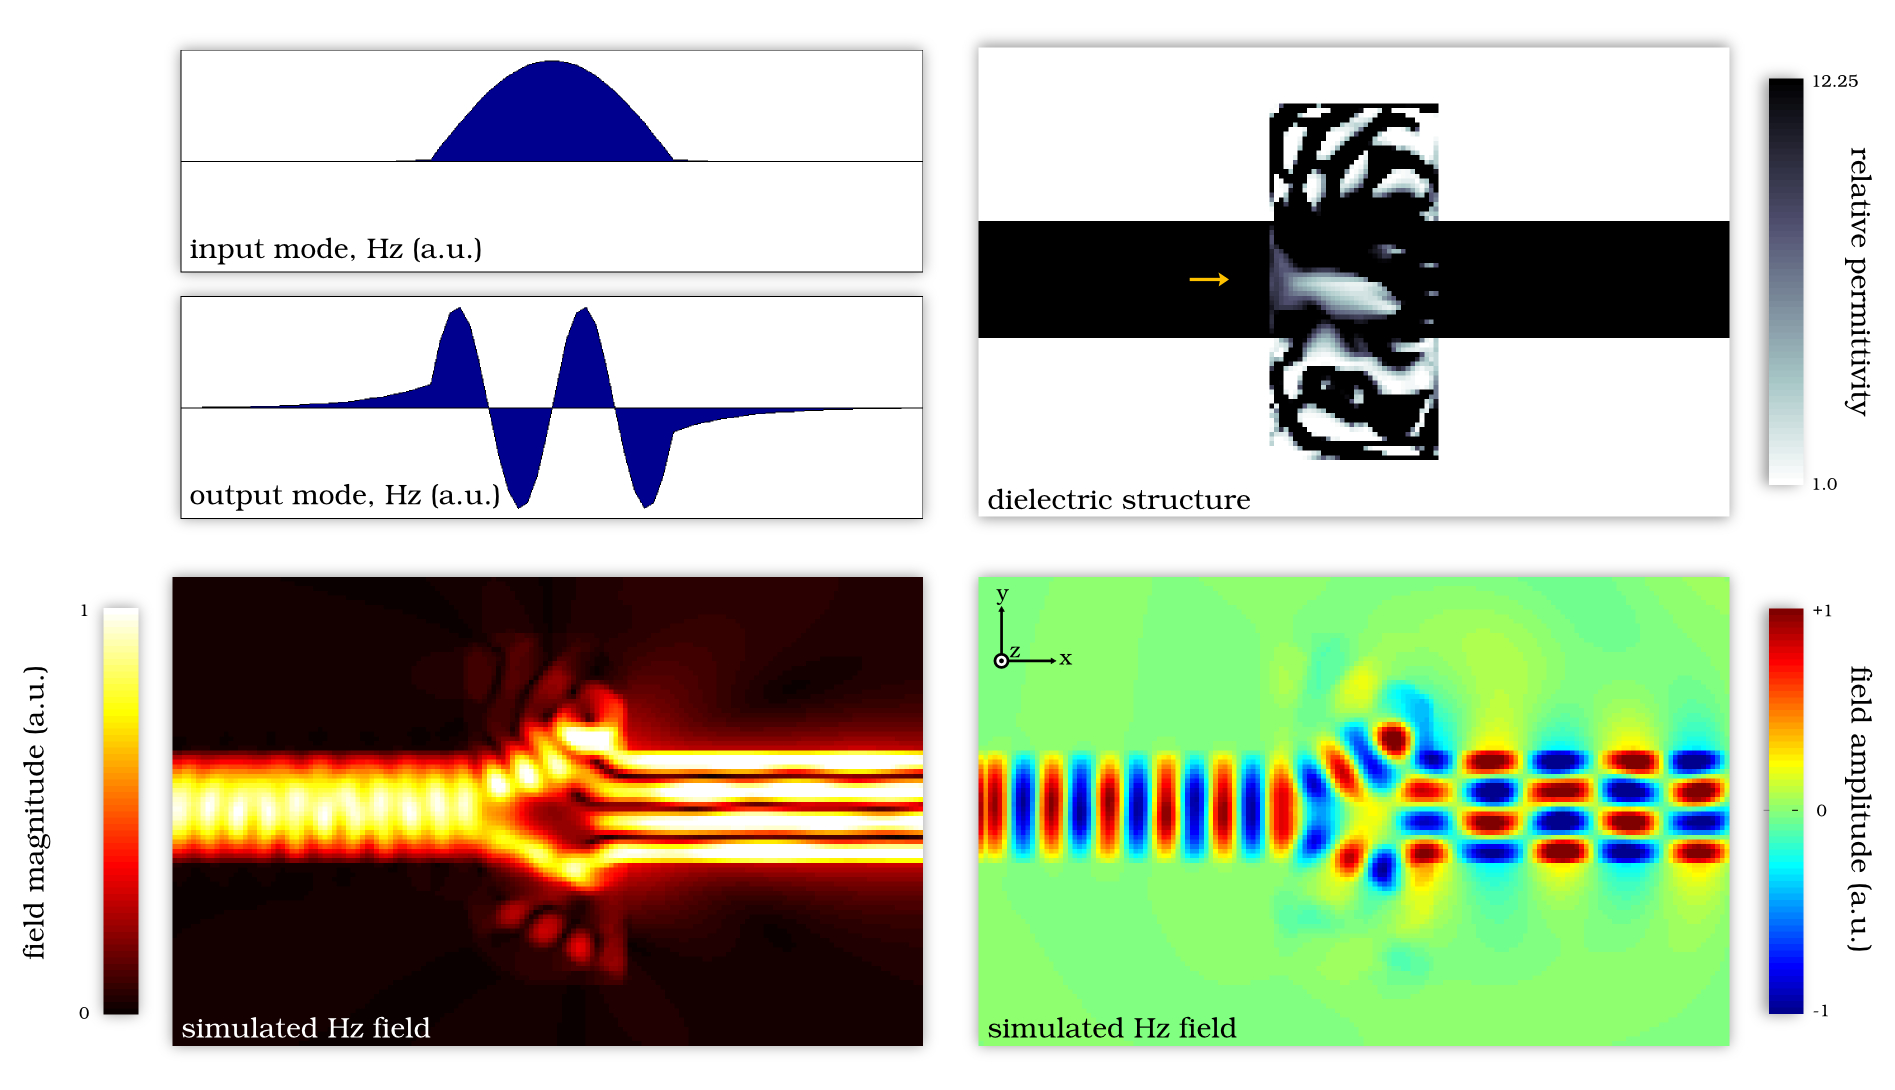
\includegraphics[width=\textwidth]{p3/8}
    \caption{
        Coupler from the first-order to the fourth-order mode 
            of a wide dielectric waveguide.
        Efficiency: $90.6\%$,
        footprint: $1.55$ square vacuum wavelengths.
        }
        % \label{fig:wire}
\end{figure}
\begin{figure}[h!]
    \centering
    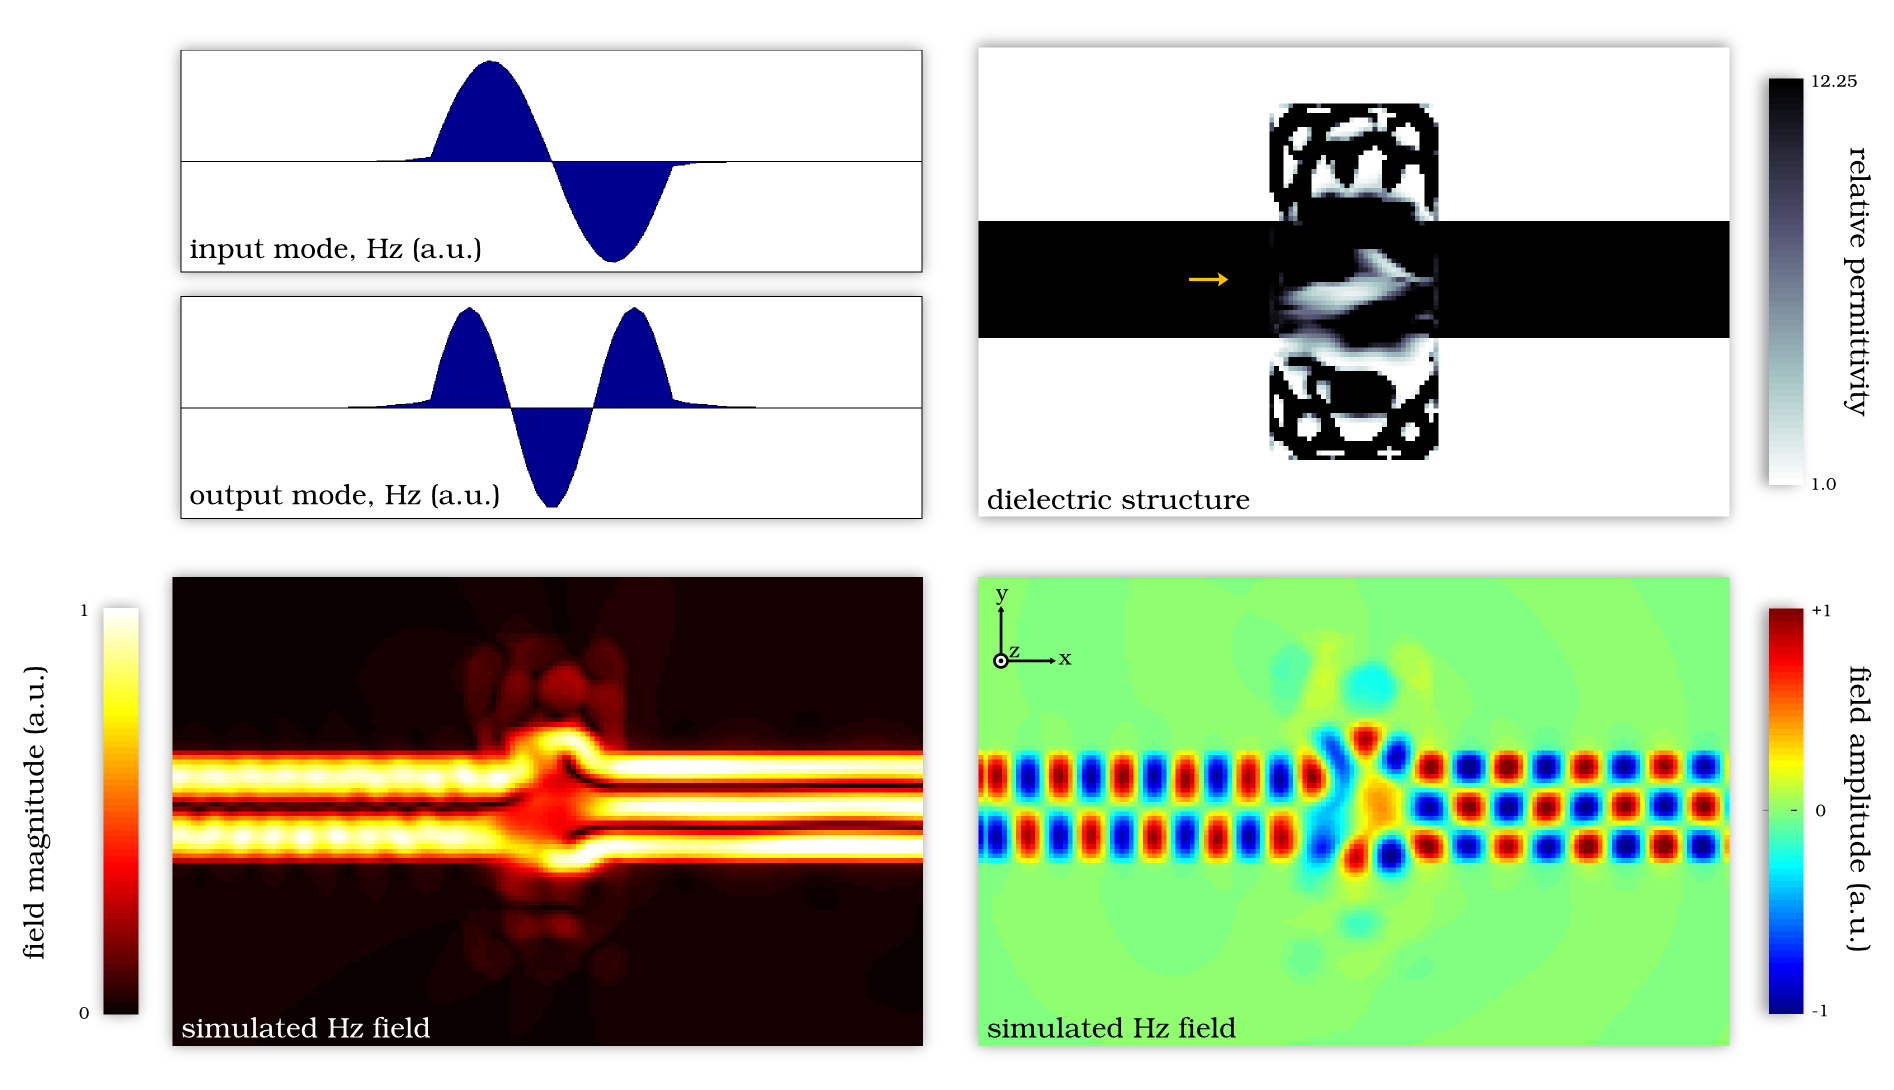
\includegraphics[width=\textwidth]{p3/9}
    \caption{
        Coupler from the second-order to the third-order mode 
            of a wide dielectric waveguide.
        Efficiency: $96.8\%$,
        footprint: $1.55$ square vacuum wavelengths.
        }
        % \label{fig:wire}
\end{figure}
\begin{figure}[h!]
    \centering
    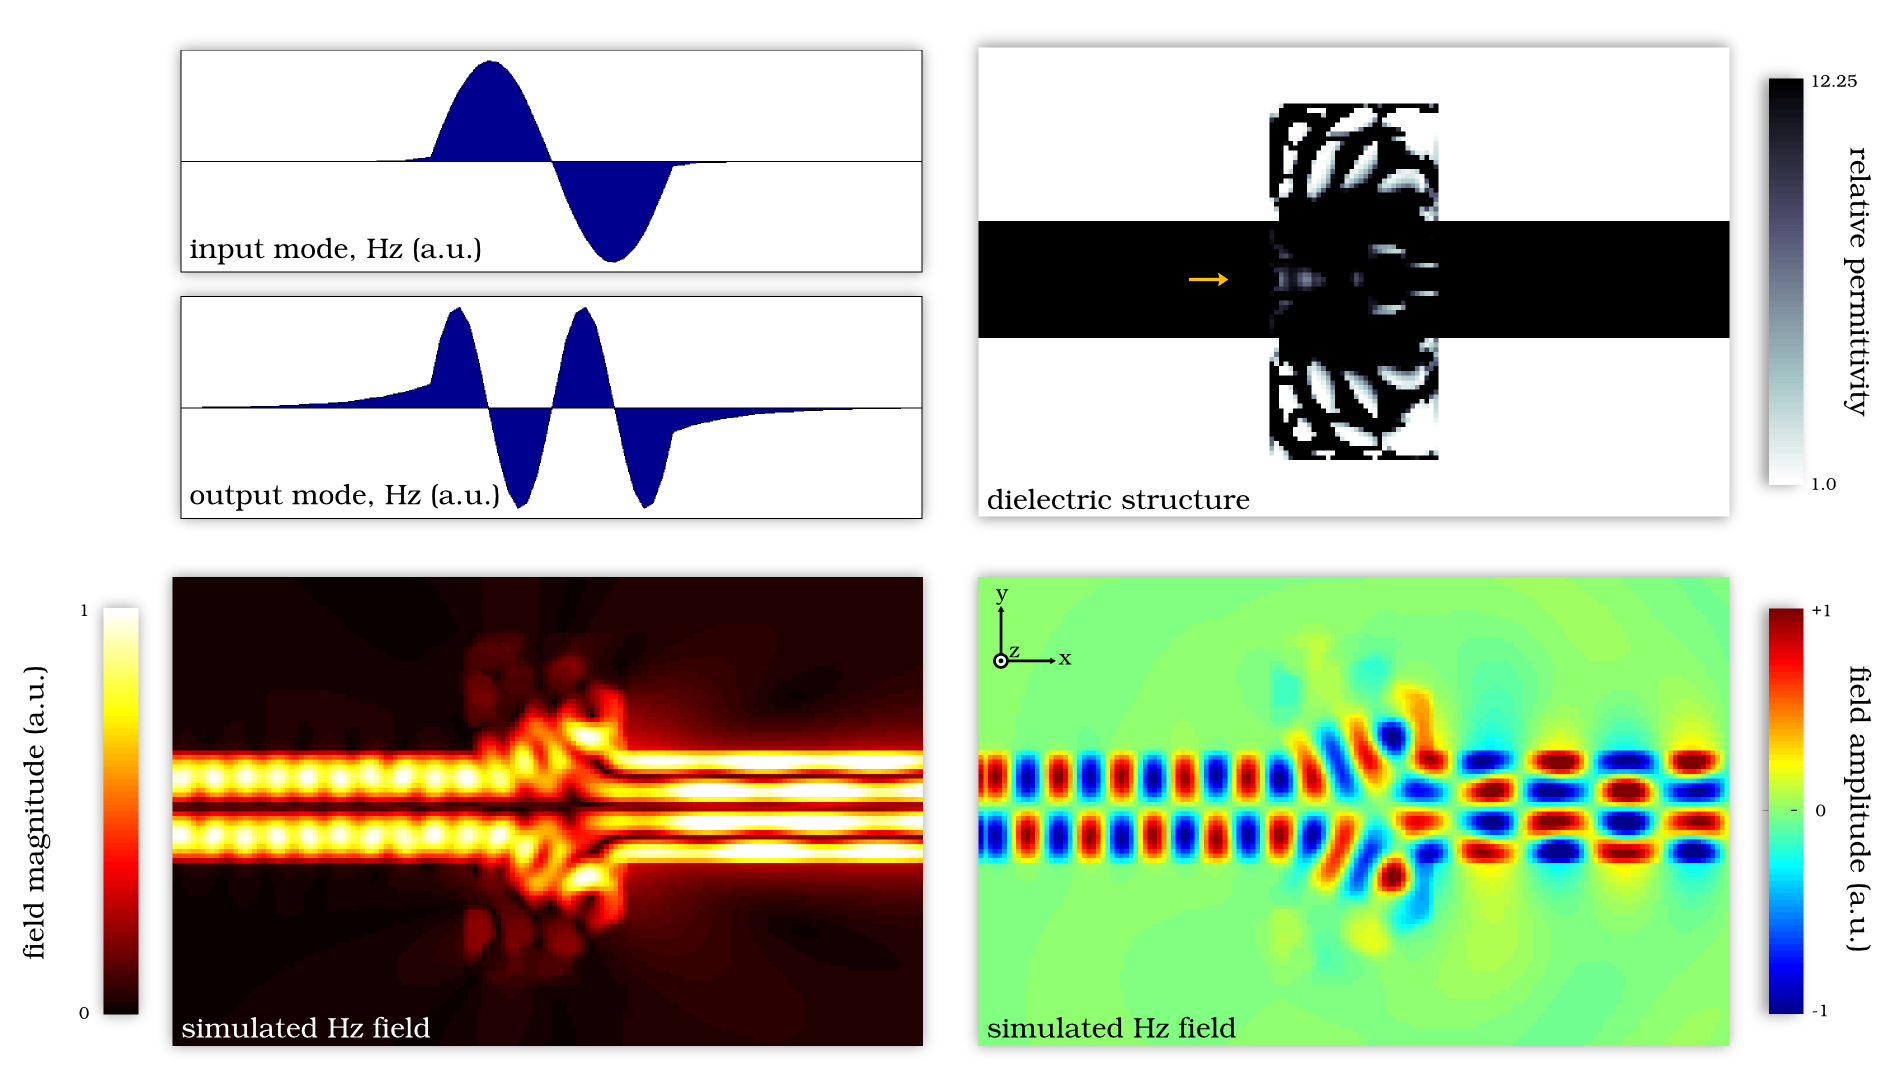
\includegraphics[width=\textwidth]{p3/10}
    \caption{
        Coupler from the second-order to the fourth-order mode 
            of a wide dielectric waveguide.
        Efficiency: $86.3\%$,
        footprint: $1.55$ square vacuum wavelengths.
        }
        % \label{fig:wire}
\end{figure}
\begin{figure}[h!]
    \centering
    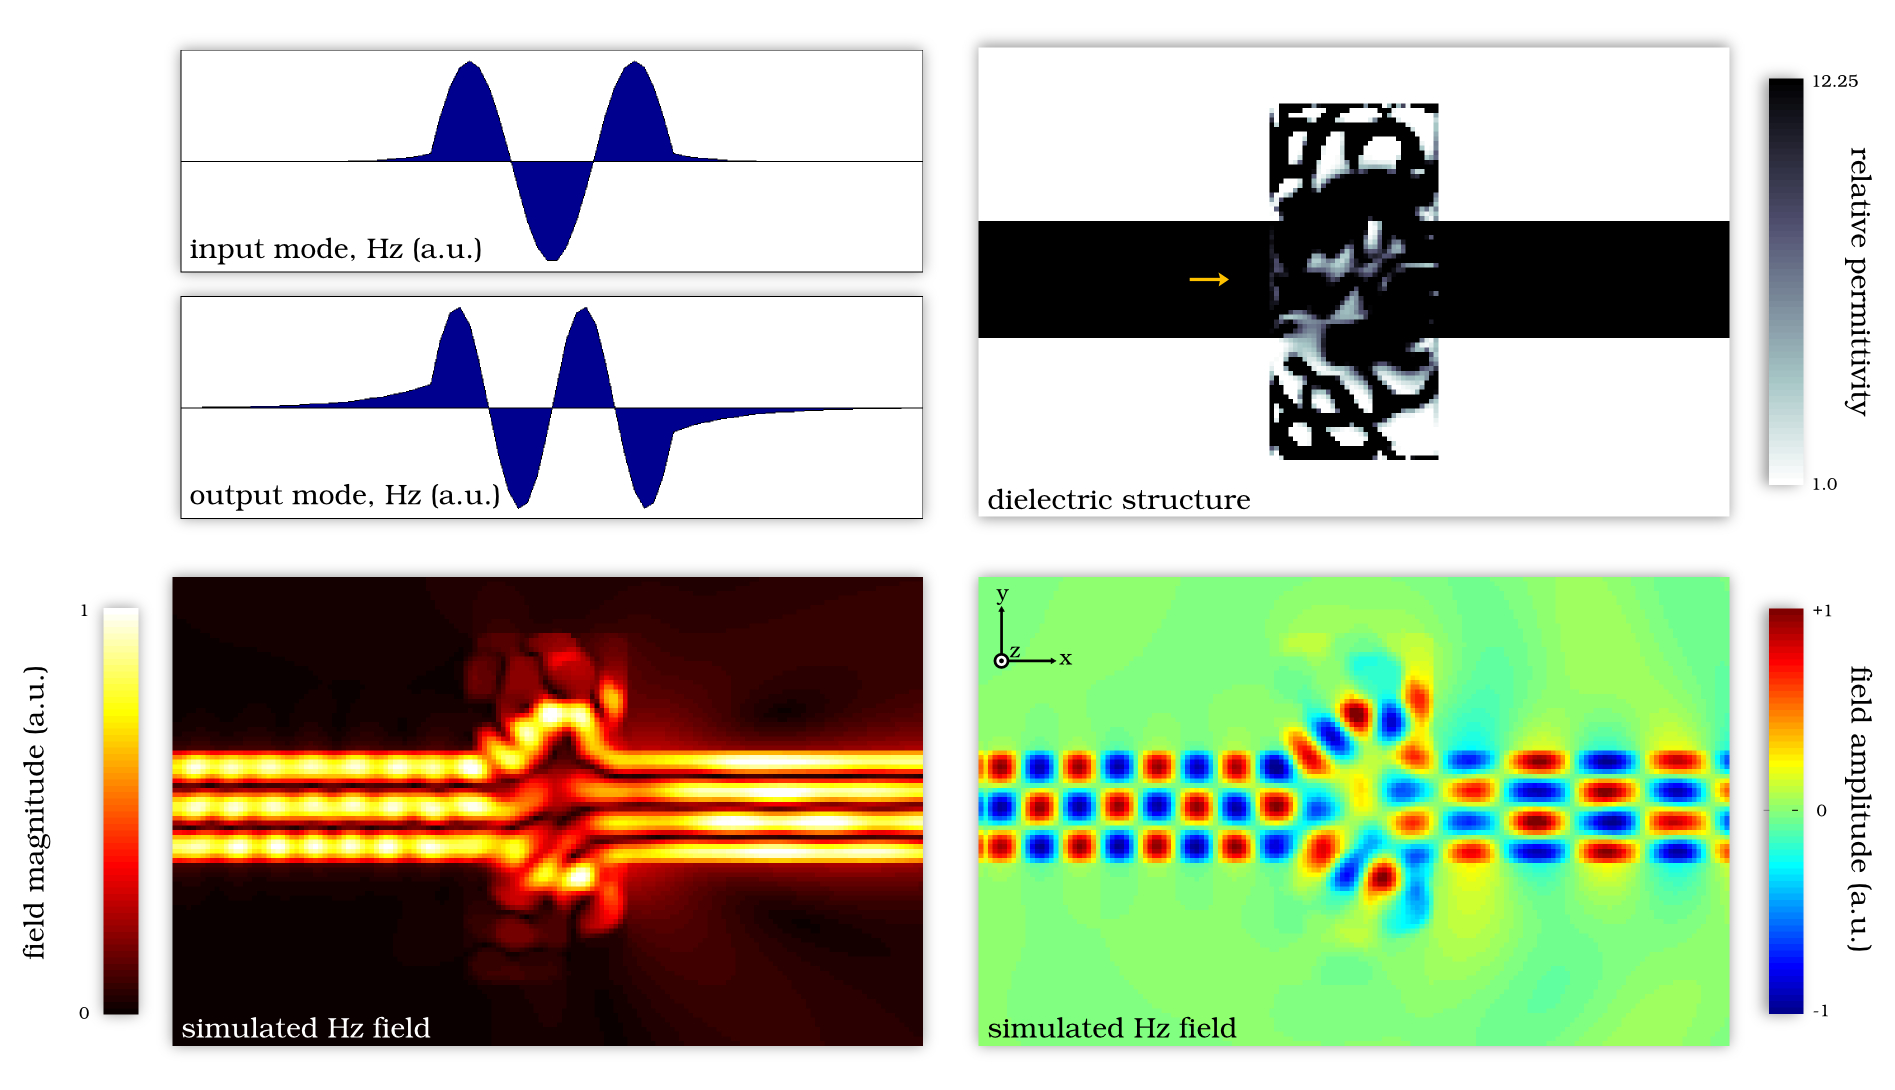
\includegraphics[width=\textwidth]{p3/11}
    \caption{
        Coupler from the third-order to the fourth-order mode 
            of a wide dielectric waveguide.
        Efficiency: $80.1\%$,
        footprint: $1.55$ square vacuum wavelengths.
        }
        % \label{fig:wire}
\end{figure}
\clearpage
\section{Additional designs with wide, low-index input waveguide}
We now reproduce Figs~\ref{fig:mode}-\ref{fig:wire}
    but instead use a wide, low-index waveguide as the input.
Once again, this is to demonstrate the generality of our method;
    namely, that it can be applied to the design of nearly any
    single-mode, linear nanophotonic device.
\begin{figure}[h!]
    \centering
    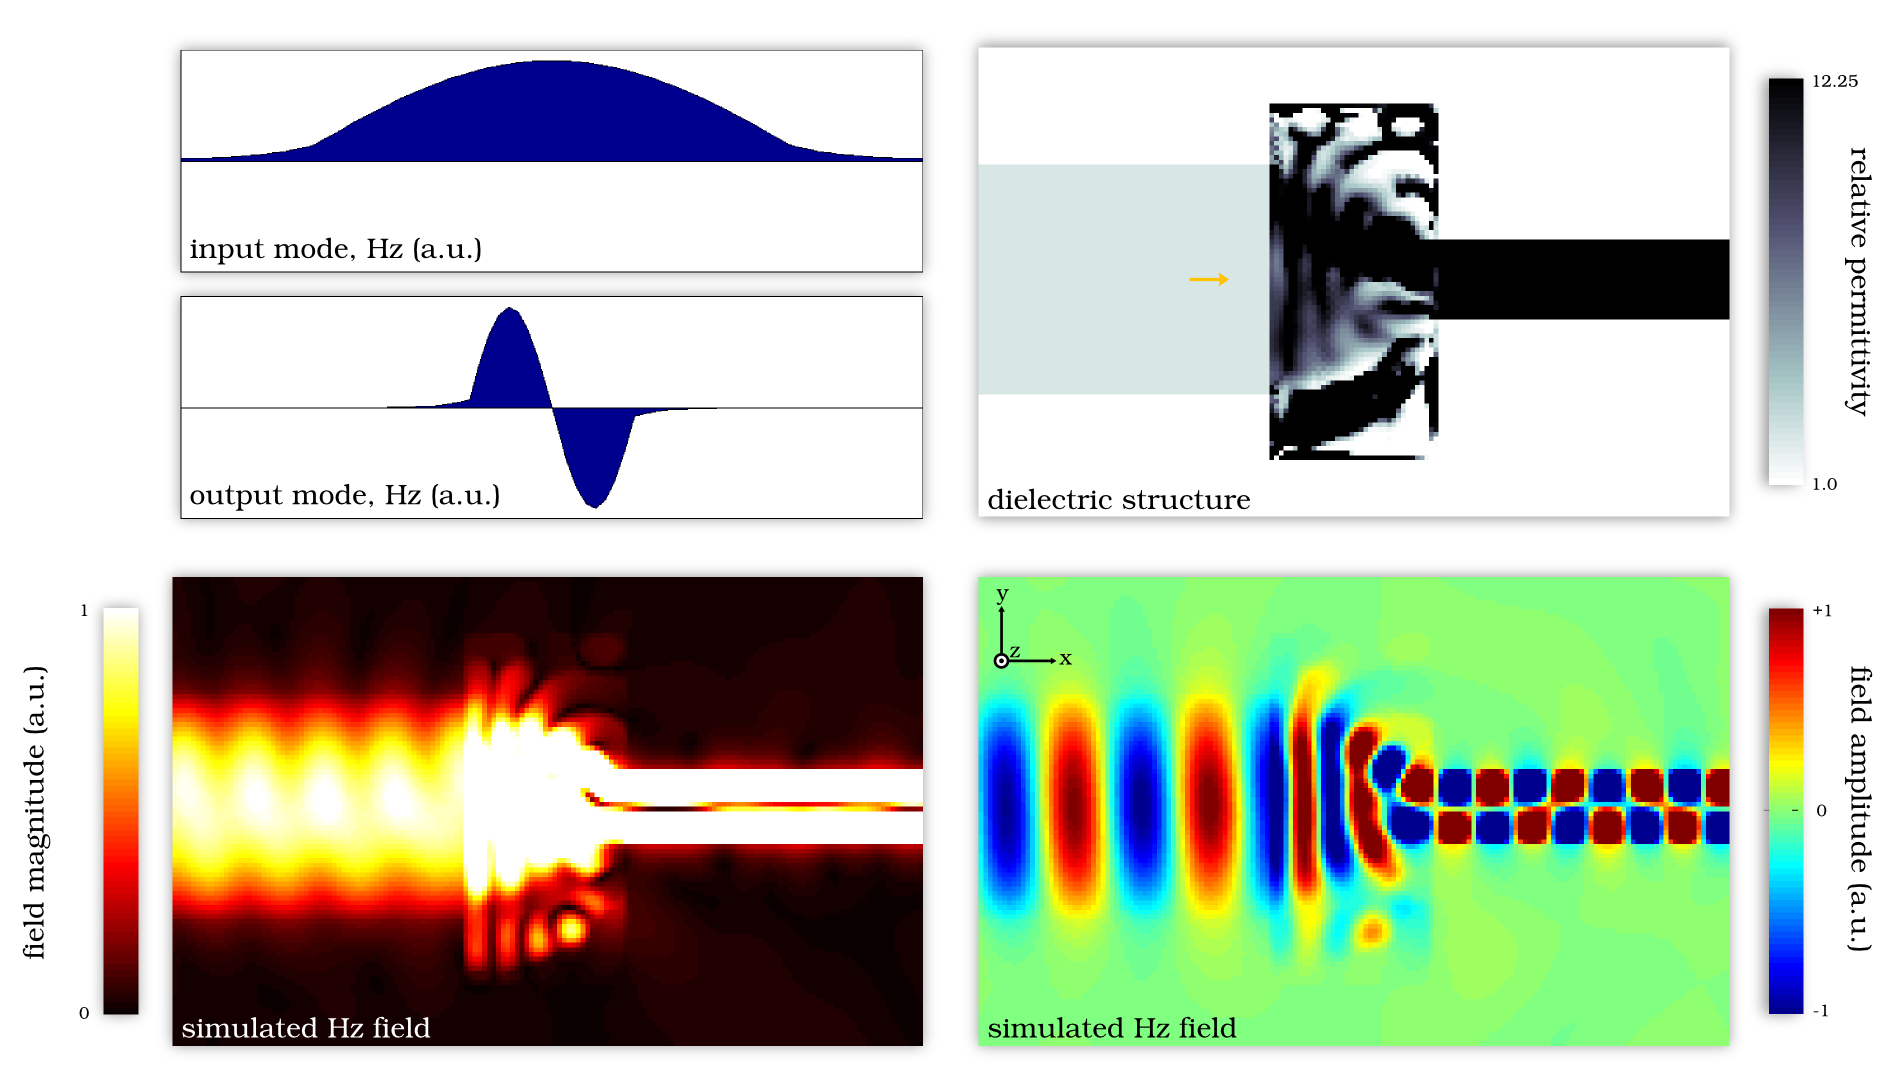
\includegraphics[width=\textwidth]{p3/12}
    \caption{
        Coupler from a wide, low-index waveguide to the
            second-order mode of a narrow, high-index waveguide.
        Efficiency: $96.9\%$,
        footprint: $1.55$ square vacuum wavelengths.
        }
        % \label{fig:wire}
\end{figure}
\begin{figure}[h!]
    \centering
    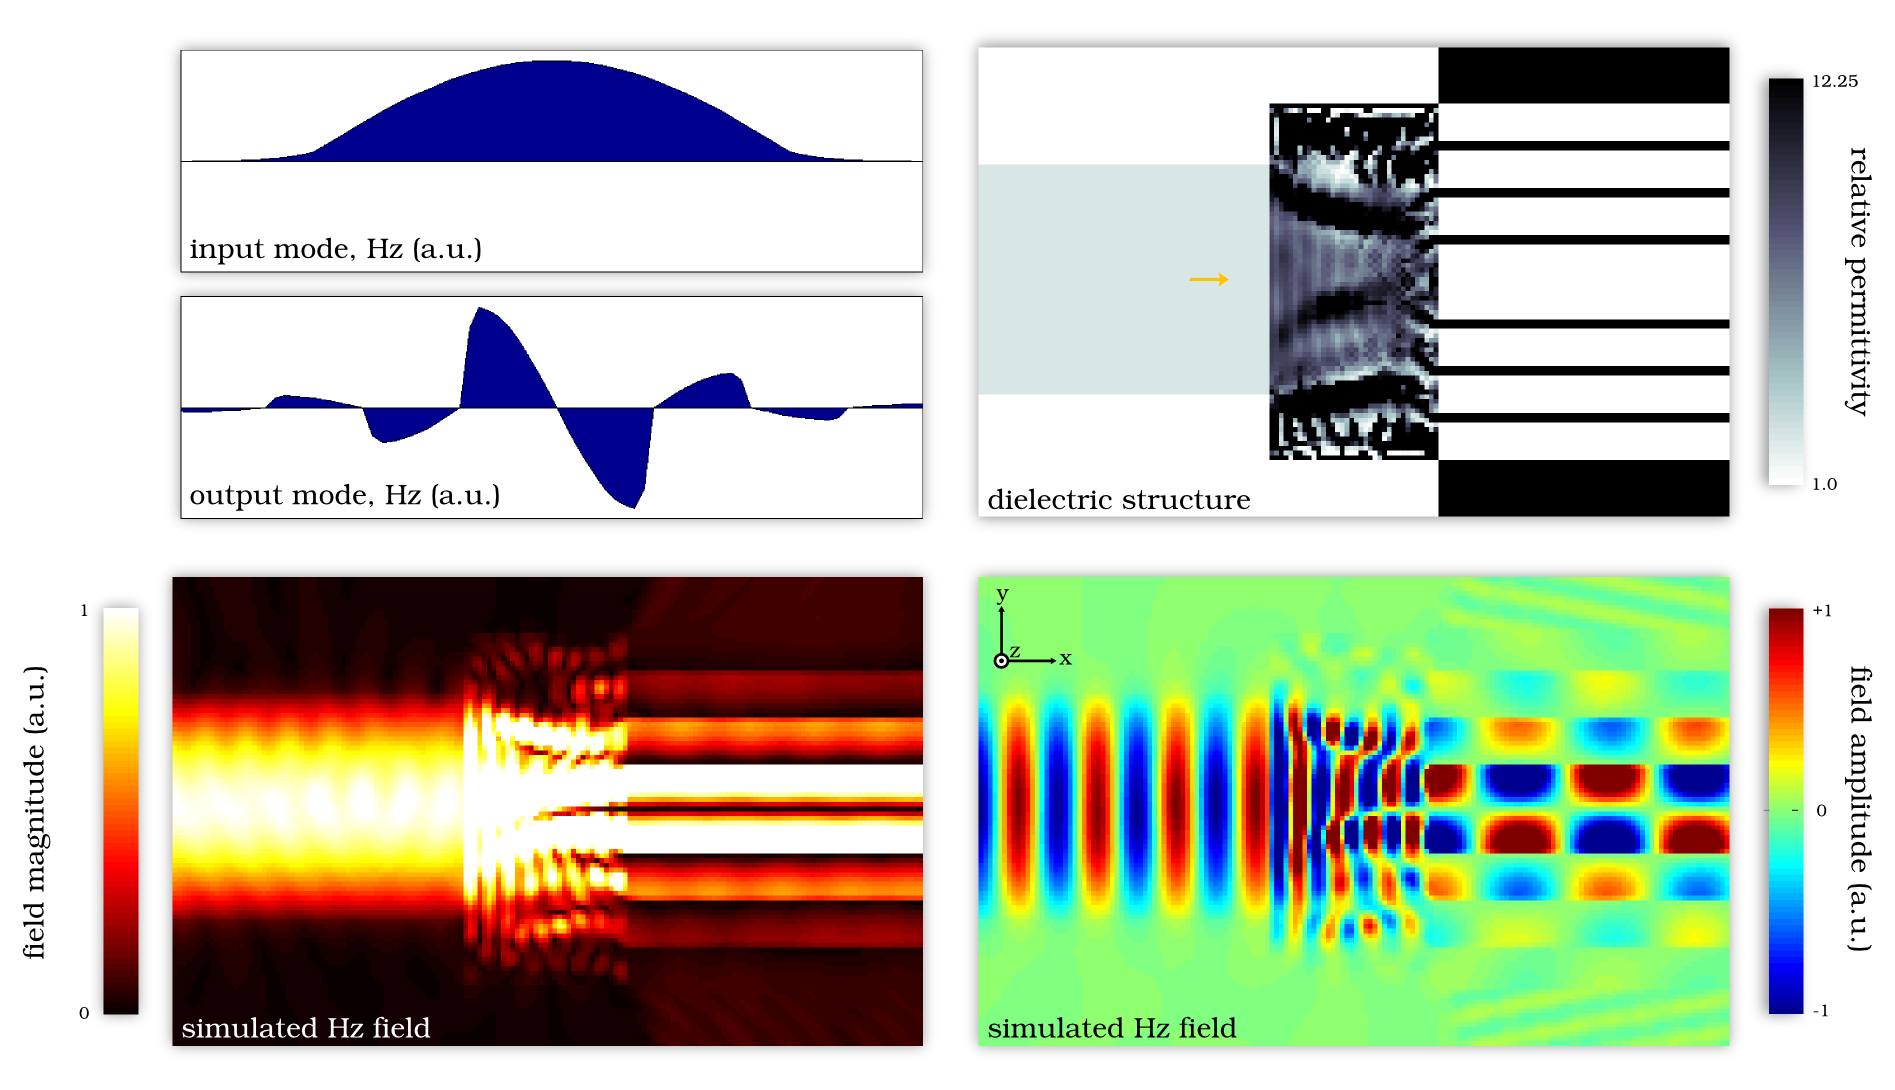
\includegraphics[width=\textwidth]{p3/13}
    \caption{
        Coupler from a wide, low-index waveguide to an 
            ``air-core'' waveguide mode.
        Efficiency: $99.0\%$,
        footprint: $4.38$ square vacuum wavelengths.
        }
        % \label{fig:wire}
\end{figure}
\begin{figure}[h!]
    \centering
    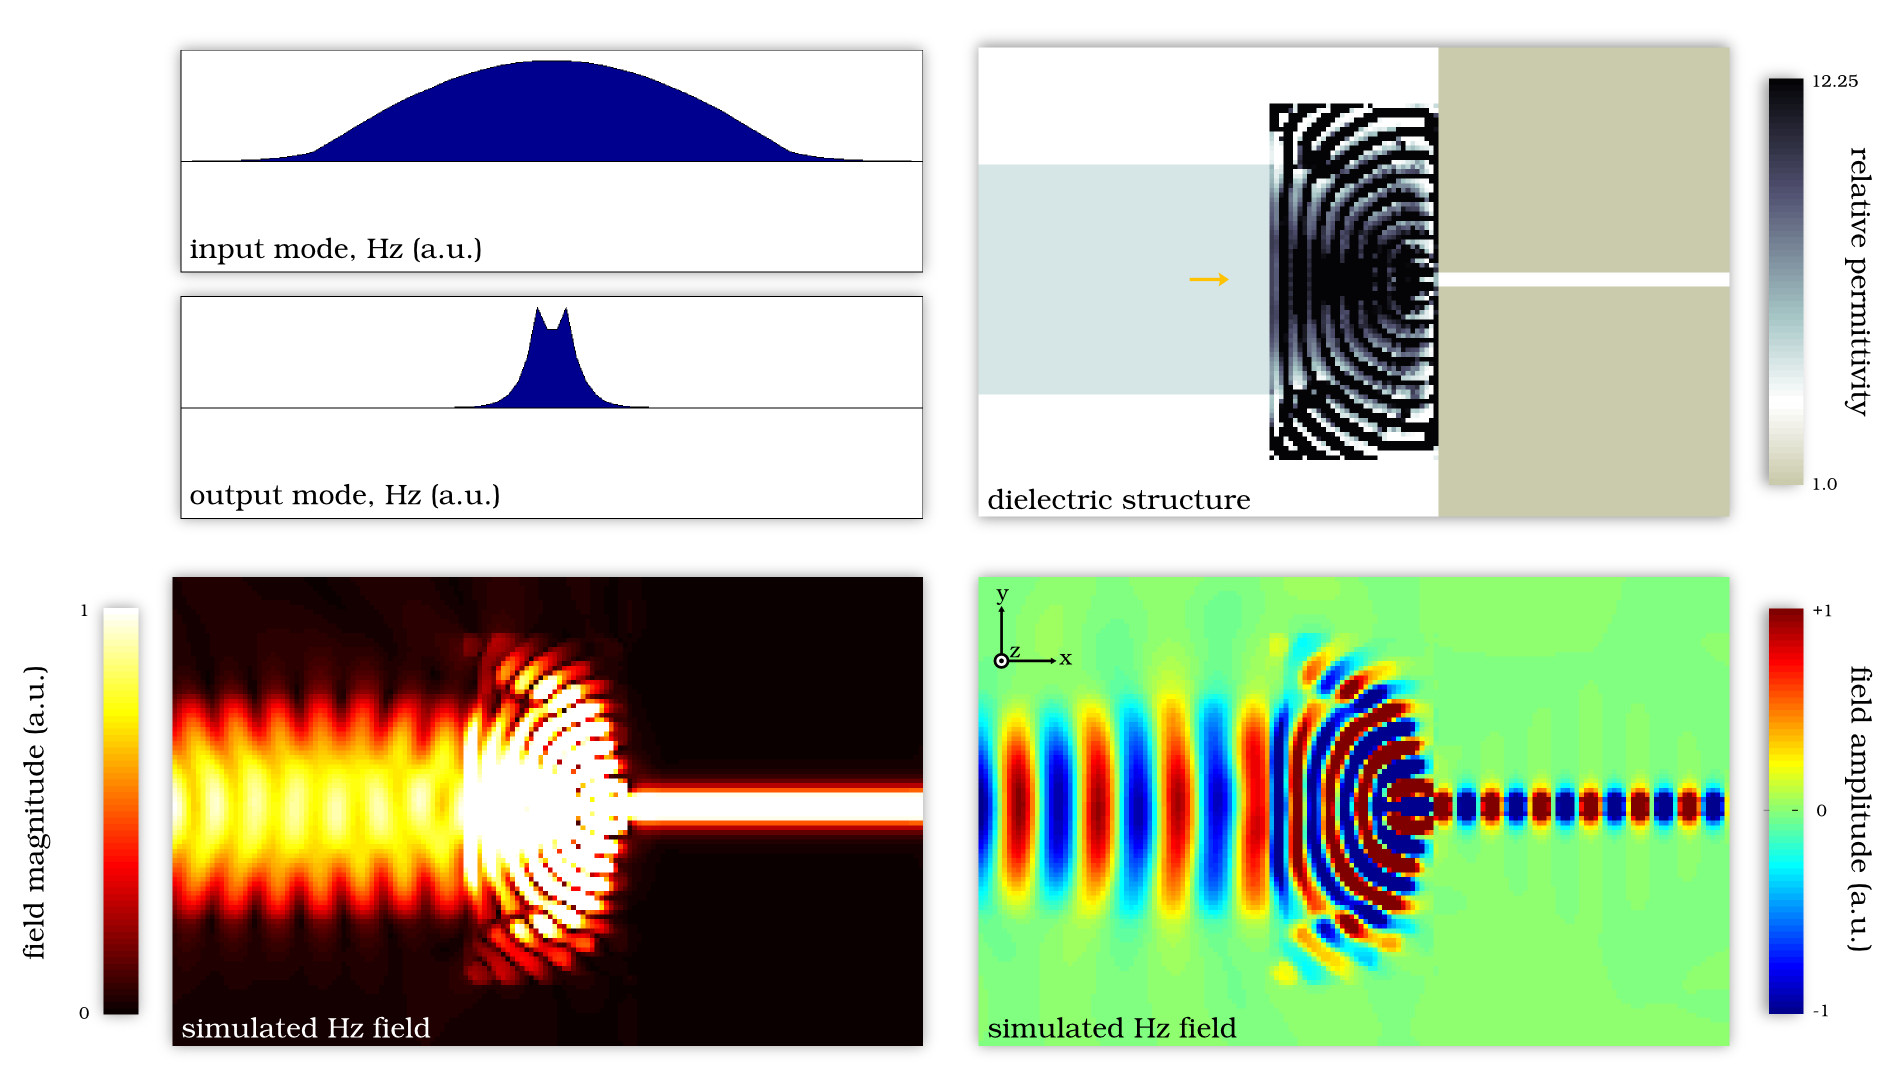
\includegraphics[width=\textwidth]{p3/14}
    \caption{
        Coupler from a wide, low-index waveguide to a
            metal-insulator-metal plasmonic waveguide mode.
        Efficiency: $96.7\%$,
        footprint: $4.38$ square vacuum wavelengths.
        }
        % \label{fig:wire}
\end{figure}
\begin{figure}[h!]
    \centering
    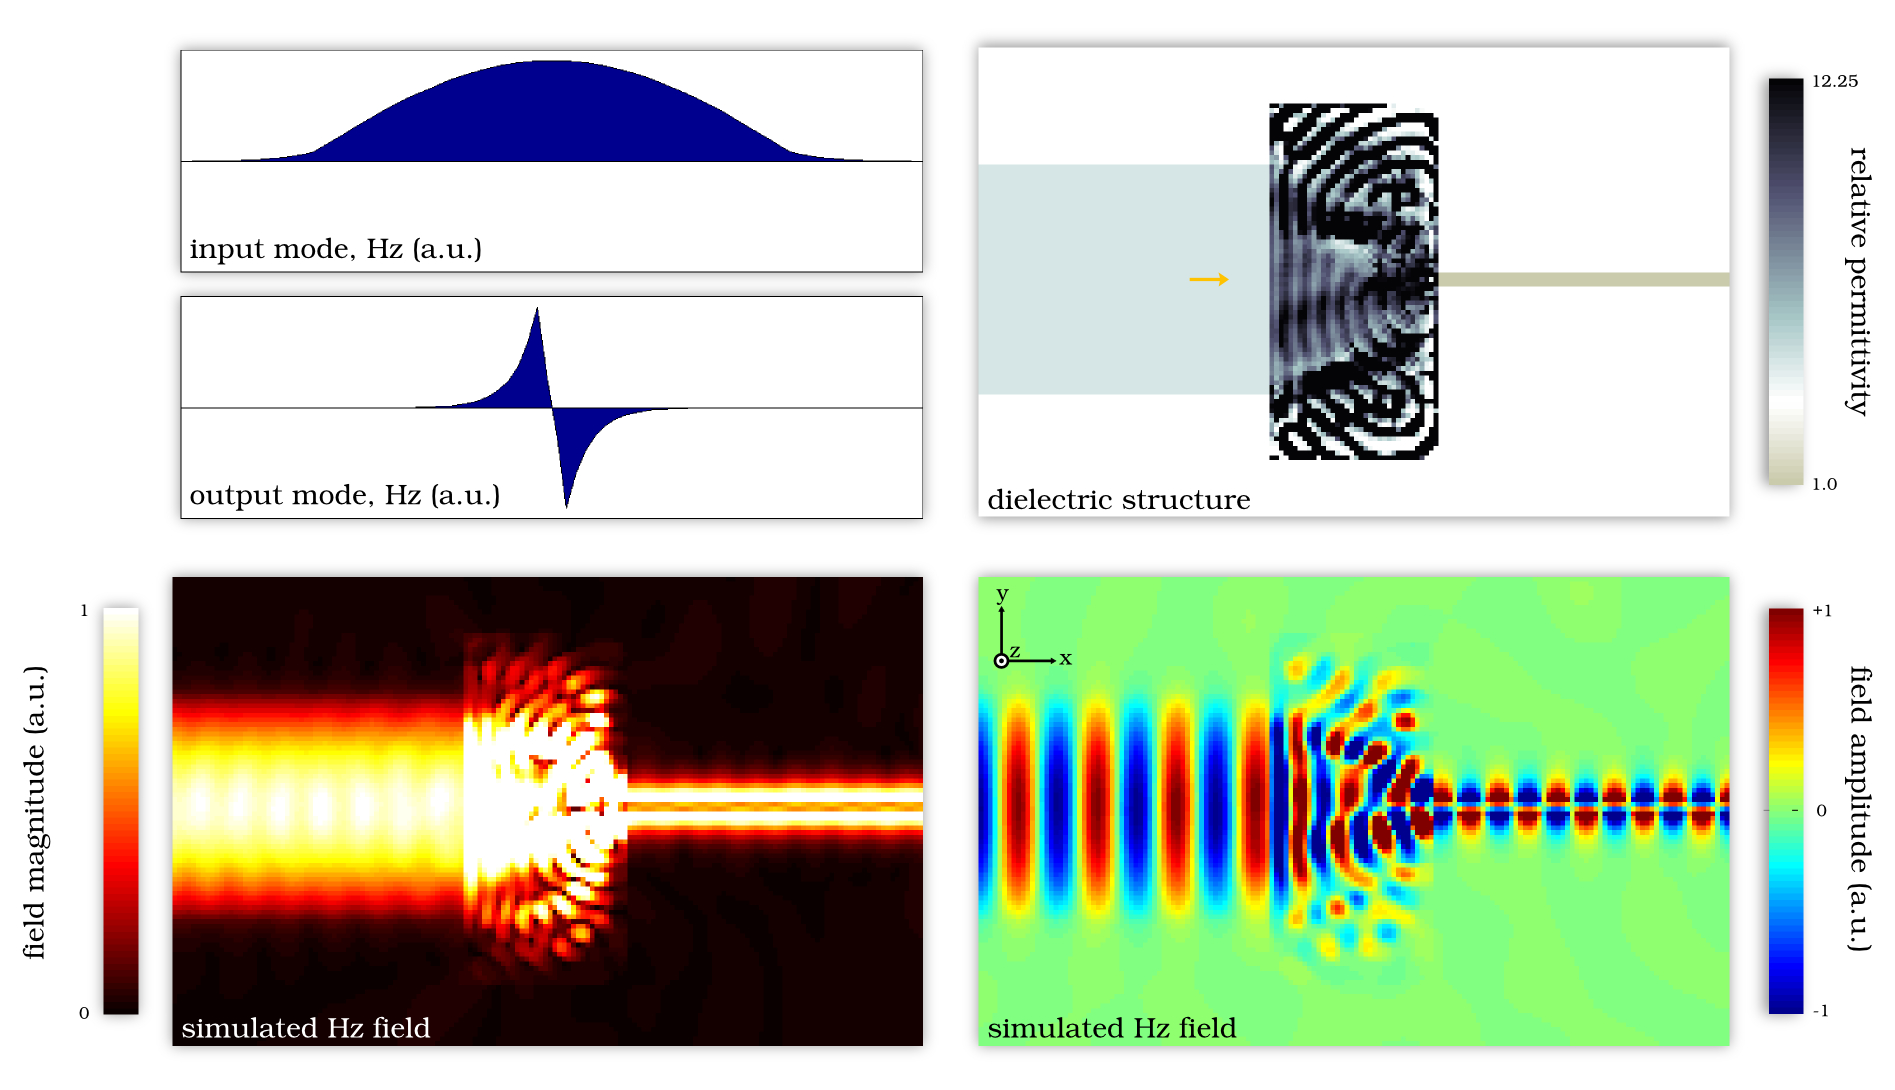
\includegraphics[width=\textwidth]{p3/15}
    \caption{
        Coupler from a wide, low-index waveguide to a
            plasmonic wire waveguide mode.
        Efficiency: $99.7\%$,
        footprint: $4.38$ square vacuum wavelengths.
        }
        % \label{fig:wire}
\end{figure}
\clearpage

\section{Additional designs with multiple output plasmonic waveguides}
We also present ``selector'' designs where photons are coupled to 
    only one of five possible plasmonic output waveguides.
We demonstrate these selector designs for both metal-insulator-metal and
    metal-wire plasmonic waveguides.
\begin{figure}[h!]
    \centering
    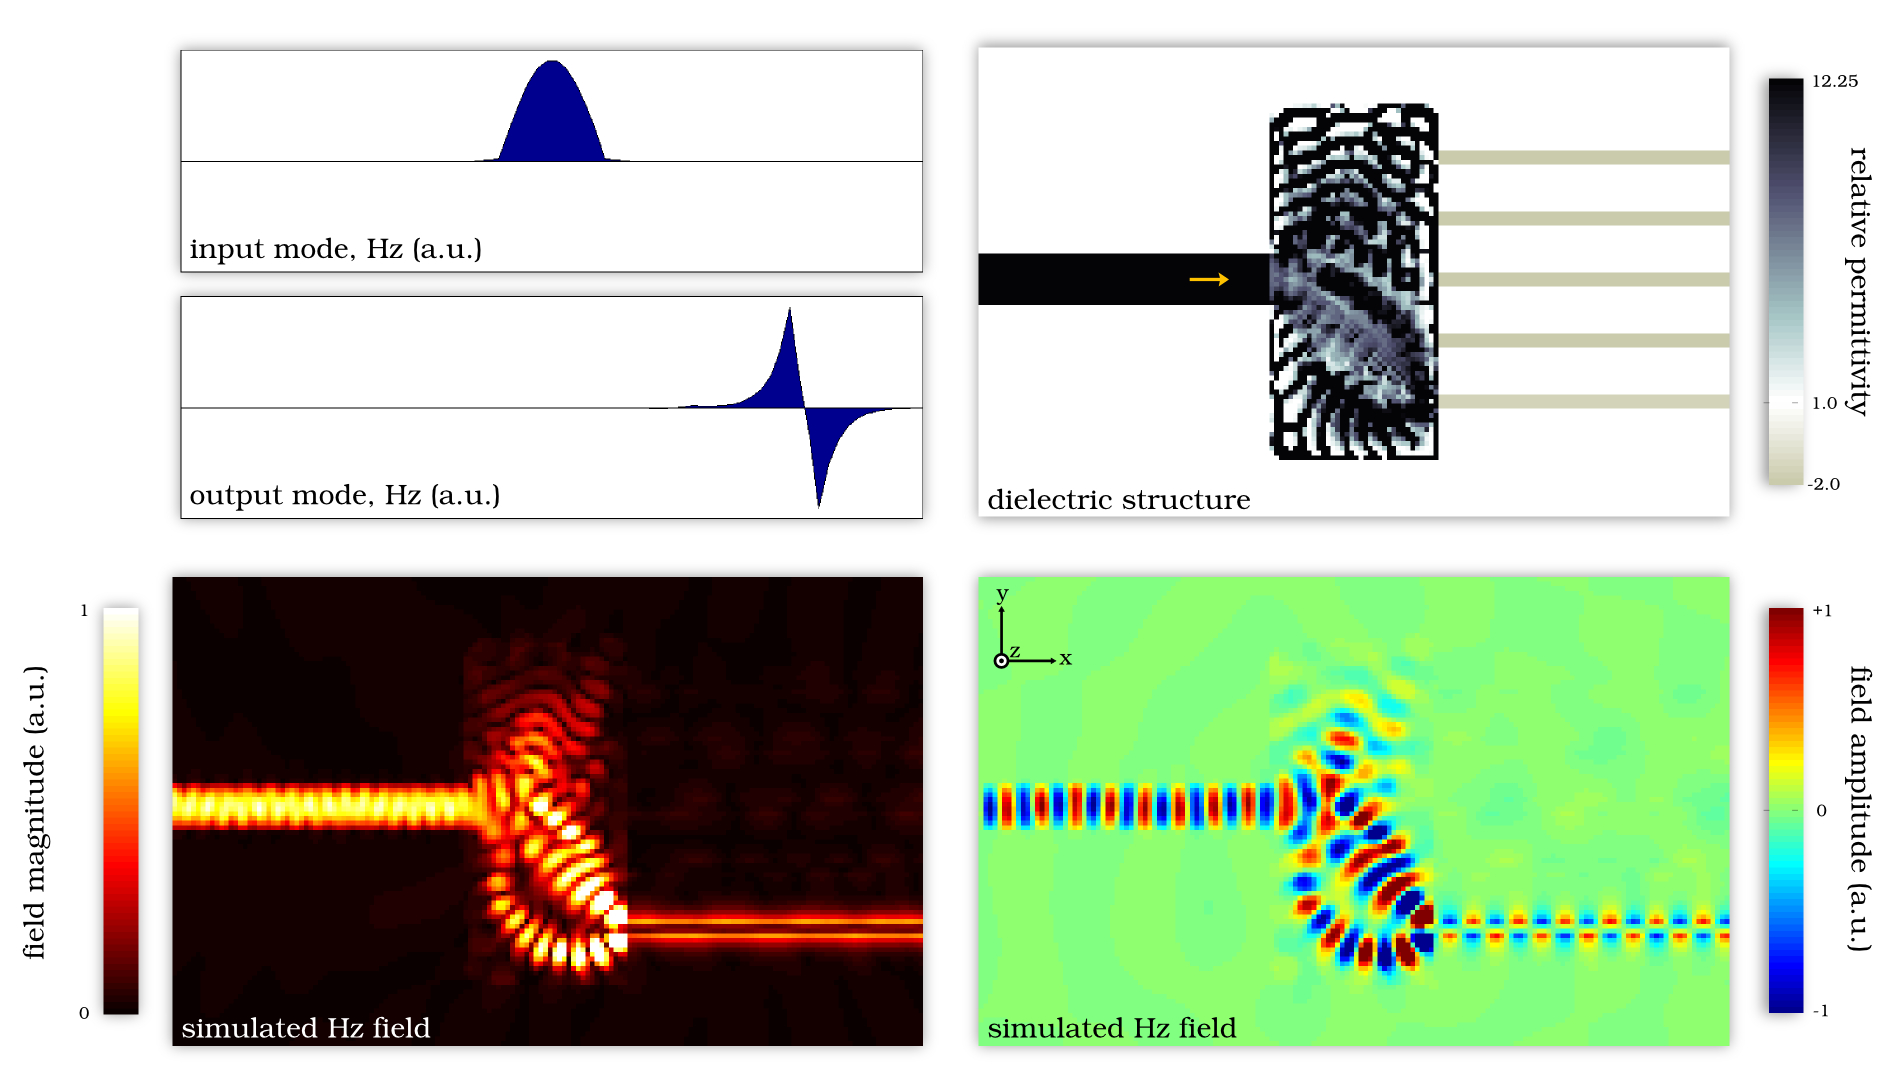
\includegraphics[width=\textwidth]{p3/16}
    \caption{
        Coupler from a dielectric waveguide to the 
            lowest branch of a set of five plasmonic wire waveguides.
        Efficiency: $94.0\%$,
        footprint: $4.38$ square vacuum wavelengths.
        }
        % \label{fig:wire}
\end{figure}
\begin{figure}[h!]
    \centering
    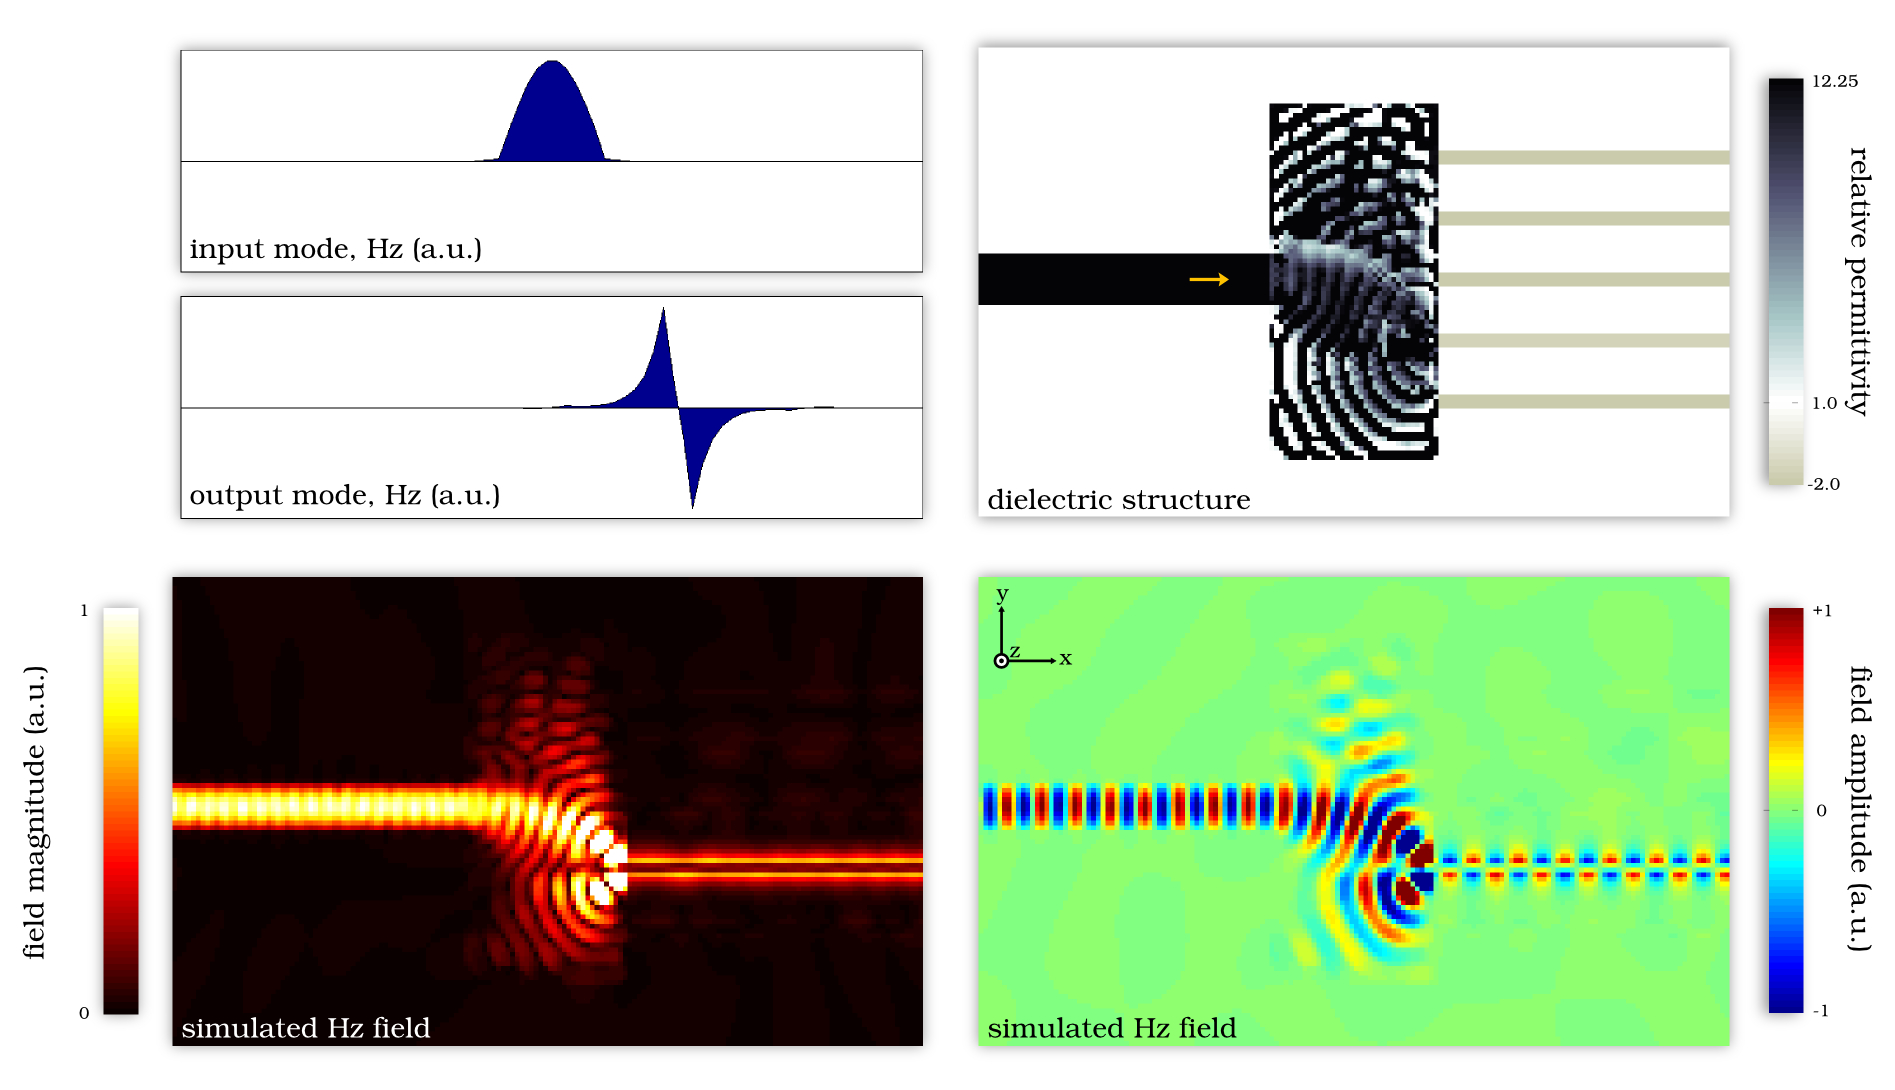
\includegraphics[width=\textwidth]{p3/17}
    \caption{
        Coupler from a dielectric waveguide to the 
            second branch of a set of five plasmonic wire waveguides.
        Efficiency: $97.3\%$,
        footprint: $4.38$ square vacuum wavelengths.
        }
        % \label{fig:wire}
\end{figure}
\begin{figure}[h!]
    \centering
    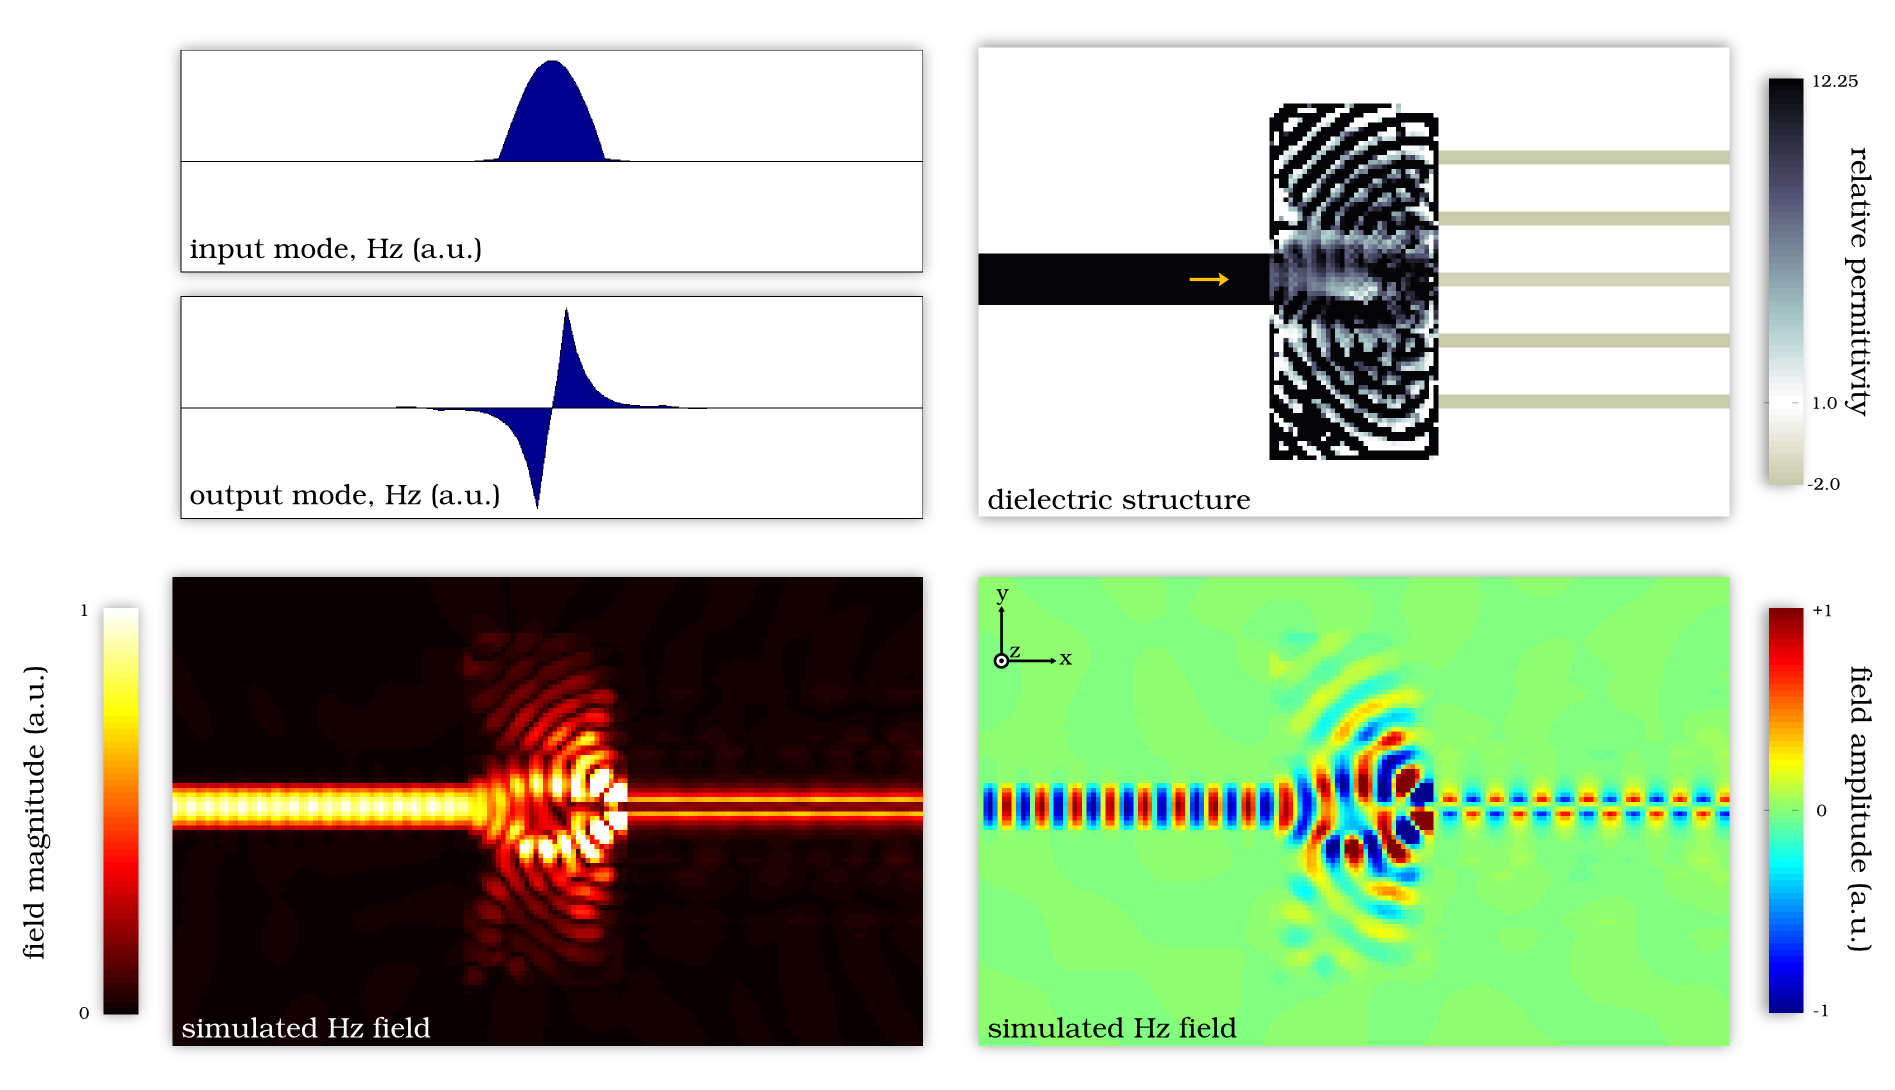
\includegraphics[width=\textwidth]{p3/18}
    \caption{
        Coupler from a dielectric waveguide to the 
            middle branch of a set of five plasmonic wire waveguides.
        Efficiency: $98.5\%$,
        footprint: $4.38$ square vacuum wavelengths.
        }
        % \label{fig:wire}
\end{figure}
\begin{figure}[h!]
    \centering
    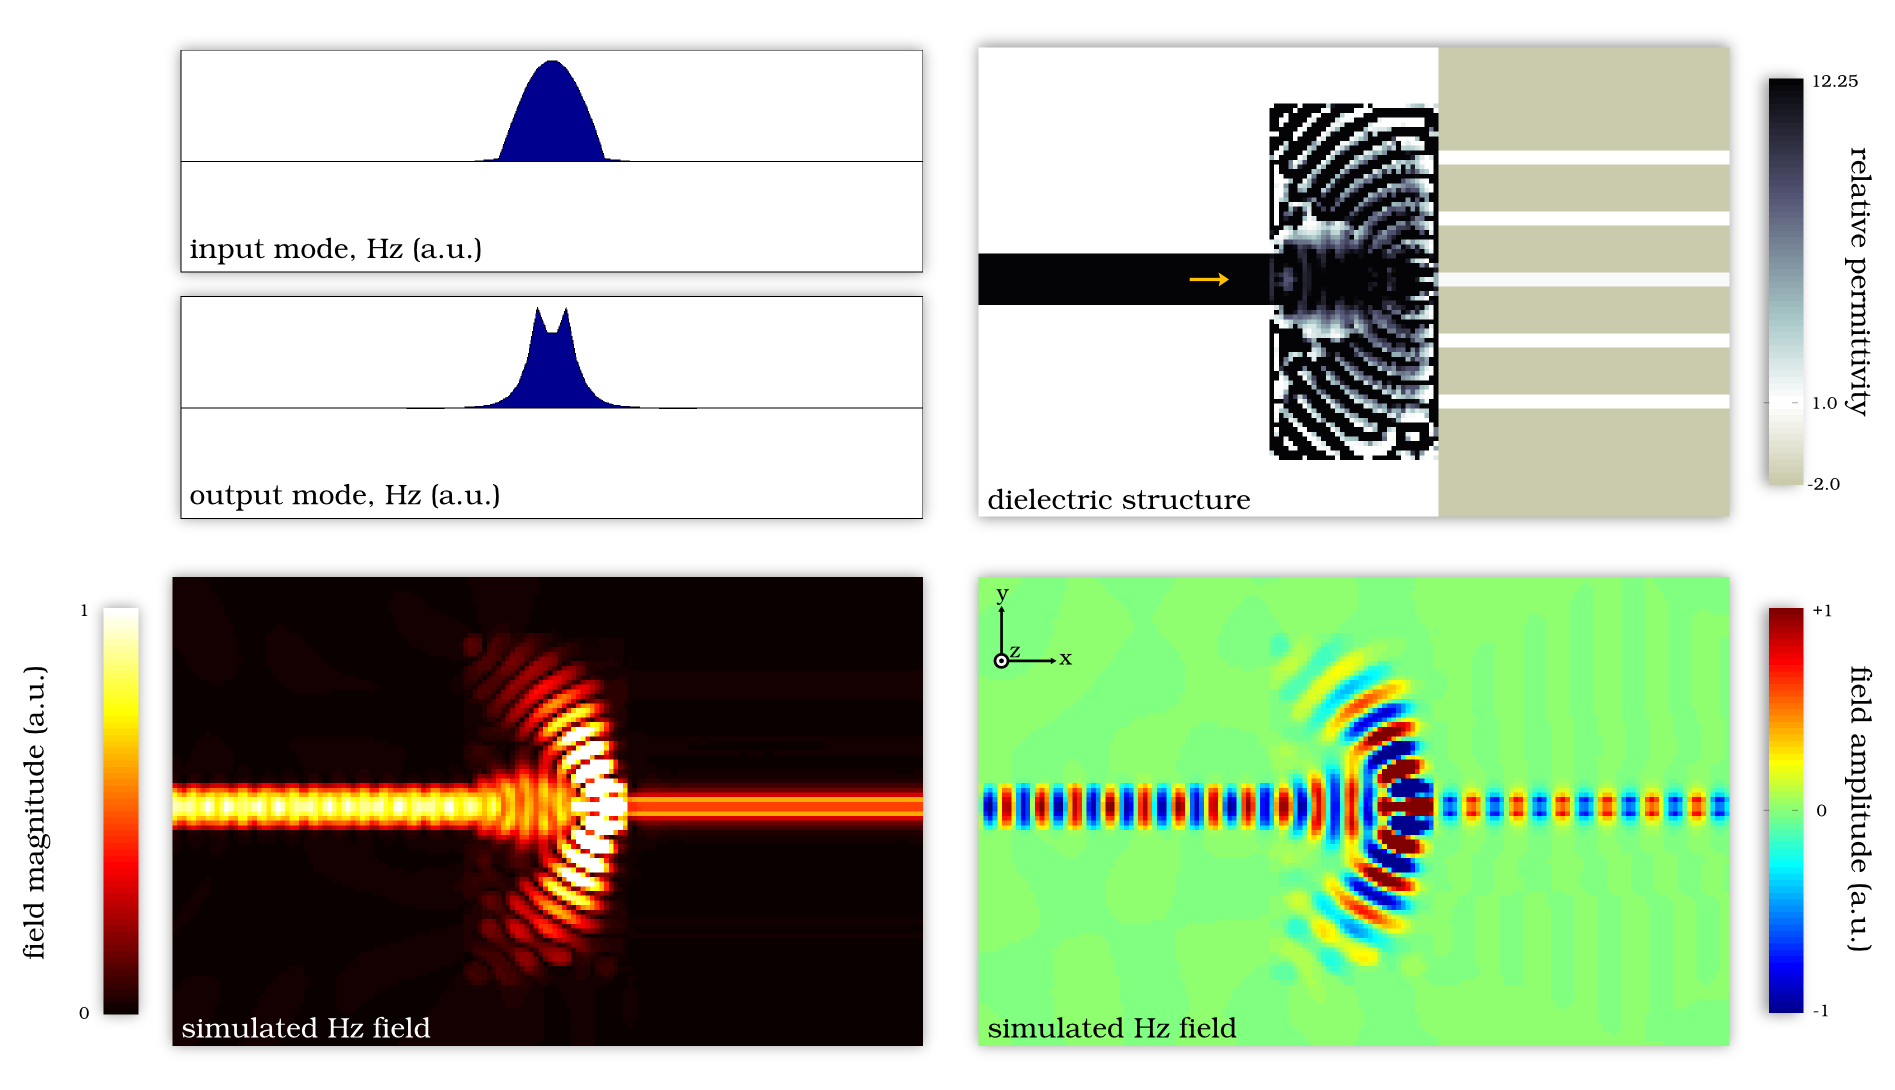
\includegraphics[width=\textwidth]{p3/19}
    \caption{
        Coupler from a dielectric waveguide to the 
            middle branch of a set of five plasmonic 
            metal-insulator-metal waveguides.
        Efficiency: $97.7\%$,
        footprint: $4.38$ square vacuum wavelengths.
        }
        % \label{fig:wire}
\end{figure}
\begin{figure}[h!]
    \centering
    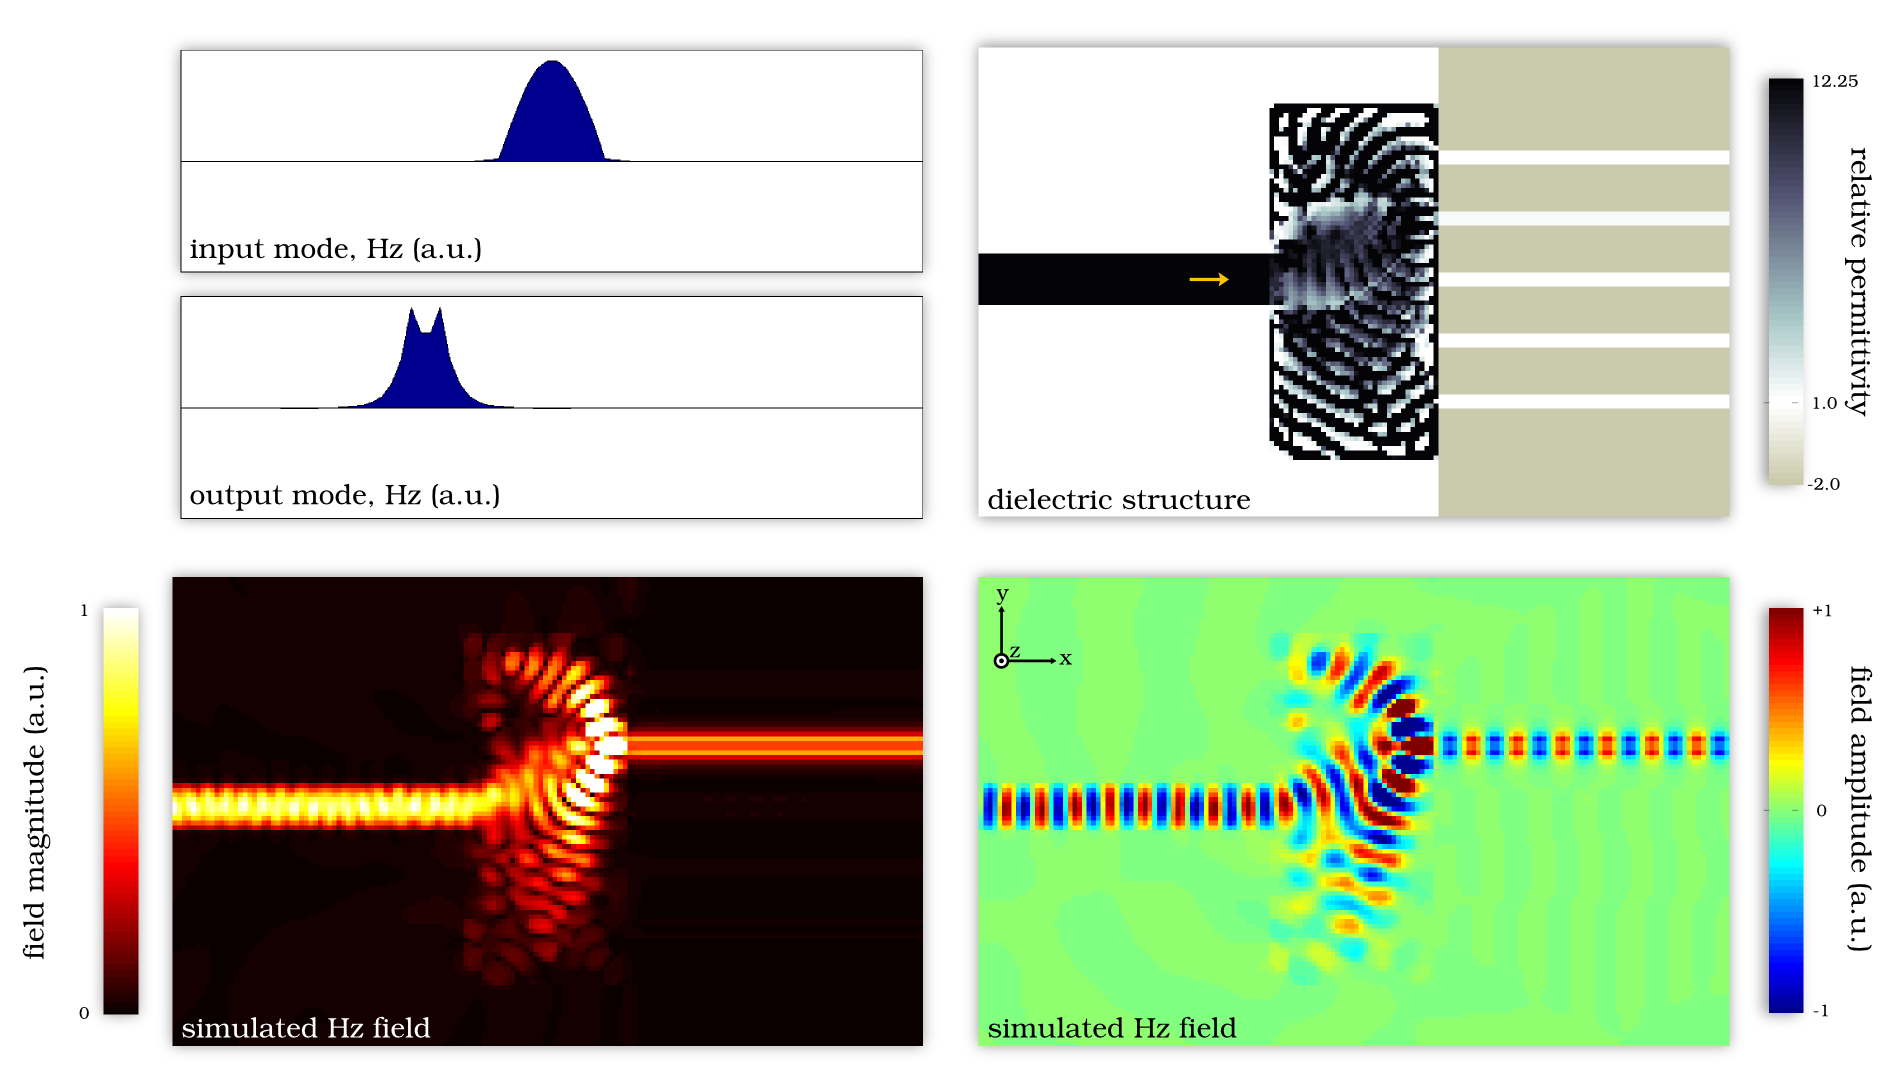
\includegraphics[width=\textwidth]{p3/20}
    \caption{
        Coupler from a dielectric waveguide to the 
            fourth branch of a set of five plasmonic 
            metal-insulator-metal waveguides.
        Efficiency: $95.6\%$,
        footprint: $4.38$ square vacuum wavelengths.
        }
        % \label{fig:wire}
\end{figure}
\begin{figure}[h!]
    \centering
    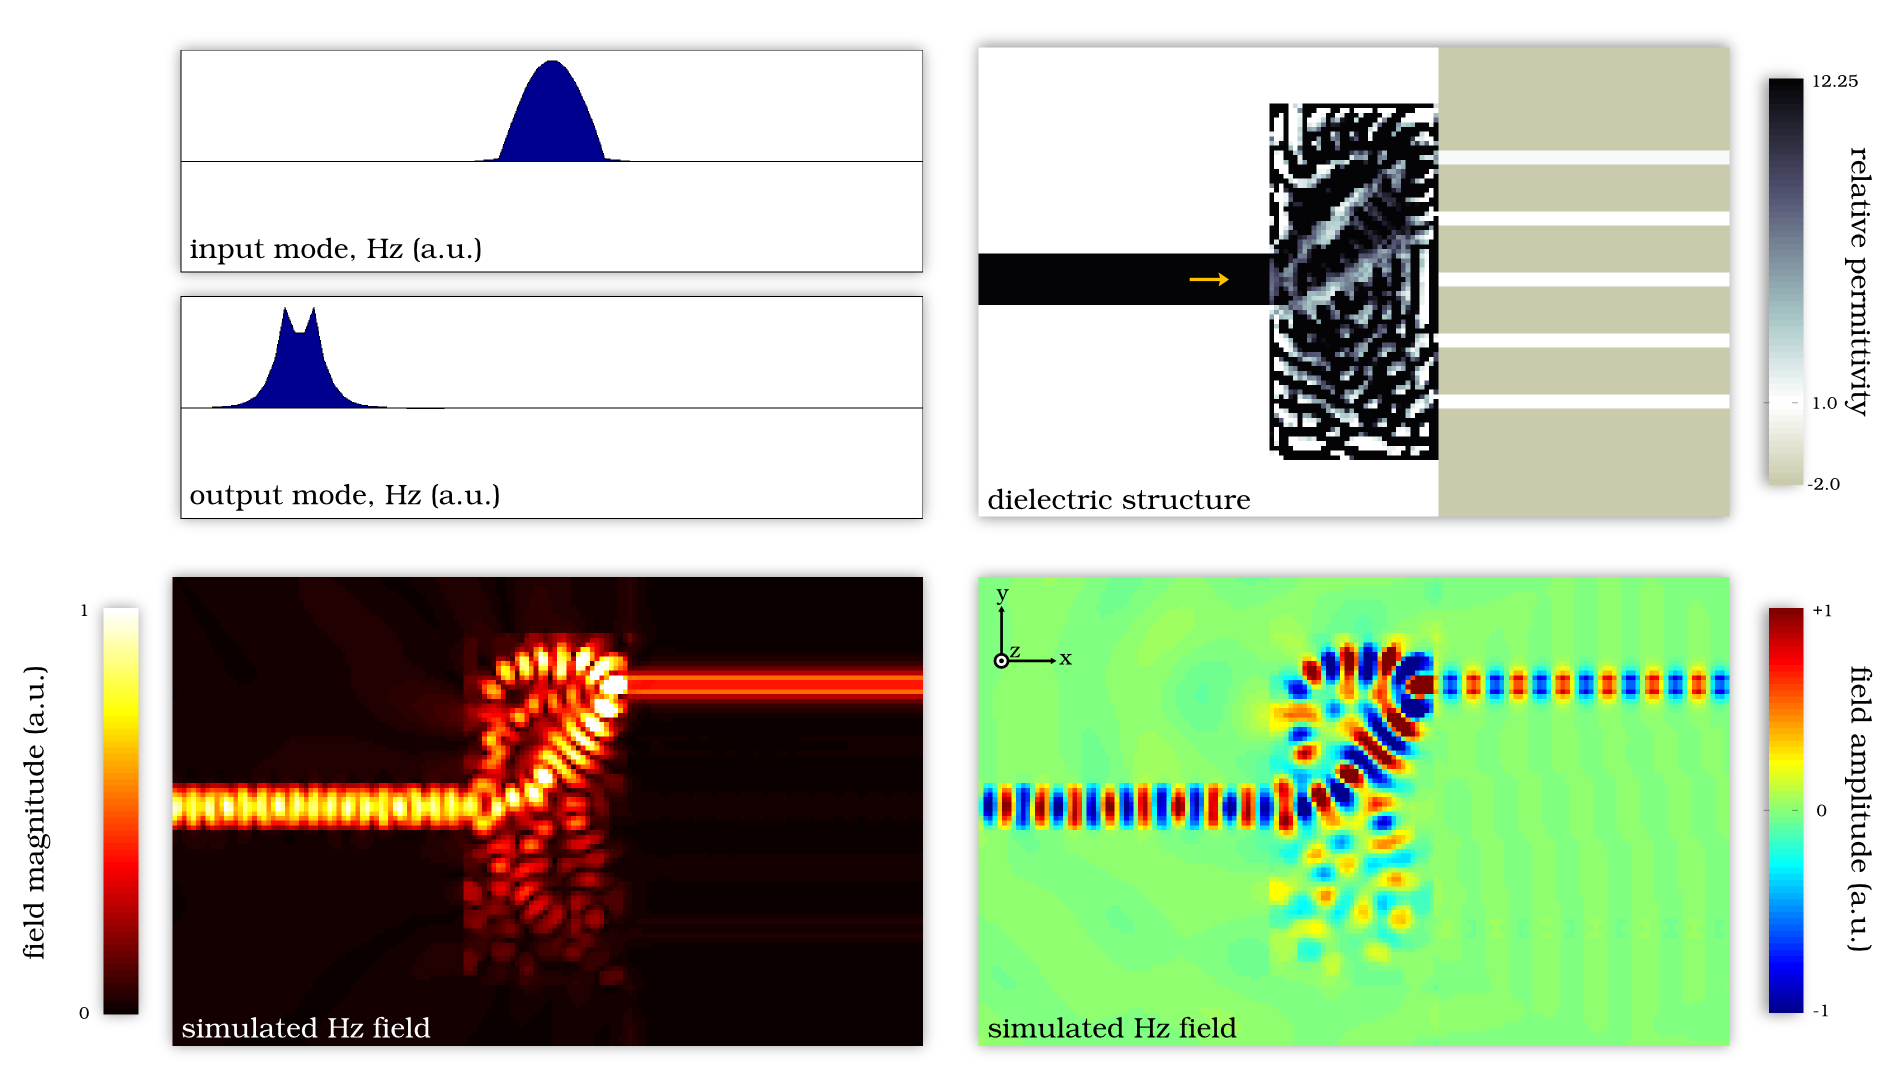
\includegraphics[width=\textwidth]{p3/21}
    \caption{
        Coupler from a dielectric waveguide to the 
            uppermost branch of a set of five plasmonic 
            metal-insulator-metal waveguides.
        Efficiency: $87.5\%$,
        footprint: $4.38$ square vacuum wavelengths.
        }
        % \label{fig:wire}
\end{figure}
\clearpage
% \end{appendix}


% \chapter{Metamaterial-like objective-first results}\label{ob-1 meta}

% \renewcommand{\eq}[1]{eq.~\eqref{eq:#1}}
\renewcommand{\EE}[2]{\begin{subequations}\begin{align}#2\end{align}\label{eq:#1}\end{subequations}}
\chapter[Computational design mathematics]{Mathematical details of nanophotonic computational design method} 
\label{maths}
As previously stated (chapter~\ref{final}), the problem we want to solve is 
    \EE {rigorous problem statement}
        {\minimize&  \sum_i^N f_i(x_i) + g(z) \\
        \subto&     A_i(z)x_i - b_i(z) = 0,\quad\text{for $i = 1, \ldots, N.$}}
To now be more precise,
    \BI $x_i \in \comps^m$ are the field variables,
    \I  $z \in \comps^n$ is the structure variable,
    \I  $f_i(x_i) \in \comps^m \to \reals$ are the field design objectives,
    \I  $g(z) \in \comps^n \to \reals$ is the structure design objective,
    \I  $A_i(z)x_i - b_i(z)$ are the physics residuals, with
    \I  $A_i(z) \in \comps^{n \times n}$ and
    \I  $b_i(z) \in \comps^n$. \EI

\section{Definition of physics residual}
The physics residual, $A_i(z)x_i - b_i(z)$, 
    corresponds to the electromagnetic wave equation
    \E  {wave equation in E}
        {(\curl \mu^{-1} \curl - \omega^2 \epsilon) E = -i \omega J}
        via
    \BI $\curl \mu^{-1} \curl - \omega^2 \epsilon \to A_i(z)$, % where $\epsilon$ is a function of $z$,
    \I  $\epsilon \to S_i z + \epsilon_{\text{const}, i}$,
    \I  $E \to x_i$, and
    \I  $-i \omega J \to b_i(z)$, typically constant with respect to $z$. \EI

\section{Bi-affine property of the physics residual}
Critically, \eq{wave equation in E} is not only linear in $E$,
    but is also affine in $\epsilon$.
This allows us to form the extremely useful relationship,
    \E  {bi-affine property}
        {A_i(z)x_i - b_i(z) = B_i(x_i)z - d_i(x_i) = 0,}
    where $B(x_i) \in \comps^{m \times n}$, $d(x_i) \in \comps^n$ and
    \BI  $-\omega^2 E \to B_i(x_i)$, 
    \I  $\curl \mu^{-1} \curl E \to d_i(x_i)$. \EI

\section{Definition of the field design objective}
Although the field design objective $f_i(x_i)$ 
    can take on virtually any form,
    we choose to define it very specifically as
    \E  {field design objective definition}
        {f_i(x_i) = \sum_j I_+(|c_{ij}\T x_i| - \alpha_{ij})
            + I_+(\beta_{ij} - |c_{ij}\T x_i|),}
    where $c_{ij} \in \comps^m$ and 
    $I_+$ is the indicator function on nonnegative reals,
    \E{}{I_+(u) = \begin{cases} 0 & u \ge 0, \\ 
                                \infty & u < 0. \end{cases}}

Such a design objective implements the constraints 
    $\alpha_{ij} \le |c_{ij}\T x_i| \le \beta_{ij}$
    which can be interpreted physically as 
    constraining the power emitted into the optical modes
    represented by $c_{ij}$.

\section{Choice of the structure design objective}
The form of the structure design objective consists of two parts,
    \BI a structure parameterization function 
        $m(p) \in \reals^l \to \comps^n$, and 
    \I  a parameter weighting function $w(p)\in \reals^l \to \reals$. \EI
Both use the variable $p$ which allows us 
    to cast $z$ into arbitrary parameters of our choice.
Together, the general form of the structure design objective is
    \E  {structure design objective definition}
        {g(z) = I_0(z - m(p)) + w(p),}
    where $I_0$ is the indicator function on the set containing only $0$,
    \E{}{I_0(u) = \begin{cases} 0 & u = 0, \\ 
                                \infty & \text{otherwise.} \end{cases}}
An alternative interpretation of \eq{structure design objective definition} 
    is that it implements a hard constraint on $z$ 
    via the parameterization function $m(z)$,
    as well as a soft constraint on $z$ 
    via the weighting function $w(z)$.

Additionally, constraints on the elements of $p$ include either
    a bounded continuous range of allowable values, or
    a finite set of discrete allowable values.



\section{Convexity analysis}
% \subsection{Joint non-convexity}
First we note that, as presented, 
    \eq{rigorous problem statement} is non-convex 
    in the variables $x_i$ and $z$. % Ref boyd book
Not only are the physics residuals $A_i(z)x_i - b_i(z)$ non-convex,
    but the field design objective, in that it implements the 
    $ \alpha_{ij} \le |c_{ij}\T x_i| $ constraint, is non-convex as well.

That our problem is non-convex means that it is fundamentally hard to solve
    because of the existence of multiple local minima.
Additionally, even if we were to arrive at the global maxima,
    we would not have a straightforward way to verify global optimality.
Lastly, fast convergence even to local minima may be difficult
    because methods such as Newton's method
    can not be directly applied to non-convex problems.

% \subsection{Separable convexity}
That said, \eq{rigorous problem statement} is \emph{separably convex} 
    in $x_i$ and $z$ if we ignore the non-convexity
    in the field design objectives, $f_i(x_i)$, and
    assume that the structure design objective, $g(z)$, is convex as well.
This is given because of the bi-affine property
    of the physics residual, as shown in \eq{bi-affine property}.

The separably convex, or \emph{bi-convex}, properties of our problem
    open the door for the use of alternating direction algorithms,
    and specifically the alternating directions 
    methods of multipliers (ADMM), % Ref. 
    for the implementation of a ``global'' optimization paradigm,
Of course, in this context we do not use the term ``global'' rigorously,
    but only to differentiate it from strategies that rely
    purely on local information.

Lastly, since our problem is not bi-convex 
    in the case of non-convex field or structure design objectives,
    simple extensions to alternating direction algorithms are employed.

% \section{Optimality condition}
% Based on the problem definition in \eq{rigorous problem statement},
%     we can write down a set of equations that, when met,
%     signal that we have arrived at a locally optimal point.
% Otherwise known as the Karush-Kuhn-Tucker (KKT) conditions, % Ref boyd
%     these are, for \eq{rigorous problem statement},
%     \EE {KKT conditions} % Check how these work out for complex values!!!
%         {|c_{ij}\T x_i| - \beta_{ij} &\le 0, \\
%         \alpha_{ij} - |c_{ij}\T x_i| &\le 0, \\
%         A_i(z)x_i - b_i(z) &= 0, \\
% %         % Lambda dual variables not needed because they do not appear 
% %         % in the last KKT condition.
% %         \lambda_{\alpha ij} &\ge 0, \\ 
% %         \lambda_{\beta ij} &\ge 0, \\
% %         \lambda_{\alpha ij}(|c_{ij}\T x_i| - \beta_{ij}) &= 0, \\
% %         \lambda_{\beta ij}(\alpha_{ij} - |c_{ij}\T x_i|) &= 0, \\
%         \nabla_z g(z) + \sum_i B(x_i)\T \nu_i &= 0,
%         }
%     where $\nu_i \in \comps^n$ are dual variables.
% 

% \chapter{The optimization module}

\section{Capabilities of the optimization software}
We have implemented various 
    \emph{optimization paradigms} and \emph{structure updates}
    which a user can arbitrarily combine in order to 
    to solve \eq{rigorous problem statement}.

Specifically, the user can choose to work in either
    a \emph{local} or \emph{global} optimization paradigm:
    \BI the local paradigm uses the adjoint method
            to find small changes in the structure which
            will decrease the design objective;
    \I  the global paradigm uses the objective-first method
            to arrive at a structure by forcing
            the design objective to be met from the start. \EI

% In addition, the user can choose between \emph{continuous} or \emph{discrete}
%     structure updates:
%     \BI a continuous update constrains the values of $p$
%         to be within a continous, bounded range; on the other hand,
%     \I  a discrete update constrains the values of $p$ 
%         within a finite set of allowable values. \EI
% 
\section{Structure of the software}

The module is naturally separated into two submodules, 
    the optimization paradigm (or simply, paradigm) submodule 
    and the structure parameterization (or simply, structure) submodule.
% The interaction between these two submodules is illustrated in \fig{strategy}.

% \begin{figure}[ht]\begin{center}
% \begin{pspicture}(6,5)(-6,-2)
% \psset{gridcolor=green, subgridcolor=yellow}
%     \let\psgrid\relax
% 
%     % Paradigm
%     \rput(0,4.3){optimization paradigm}
%     \psline(-2.2,4)(2.2,4) % top
%     \psline(-2.2,4)(-2.2,2) % left
%     \psline(2.2,4)(2.2,2) % right
%     \psline(-2.2,2)(-1,2)
%     \psline(2.2,2)(1,2)
%     \psline(-1,2.2)(1,2.2)
%     \psline(-1,2)(-1,2.2)
%     \psline(1,2)(1,2.2)
% 
%     % Parameterization
%     \psframe(-.8,0.8)(.8,-0.4) 
%     % \rput[t](0,-0.6){\parbox{3cm}{\center structure\\ update}}
%     \rput[t](0,-0.6){structure update}
% 
%     % Arrows
%     \rput[r](-4.3,3){$z_\text{init}$}
%     \psline{->}(-4,3)(-2.4,3)
% 
%     \rput[r](-1.9,0.8){$Q(z)$}
%     \psline(-1.6,1.8)(-1.6,0.2)
%     \psline{->}(-1.6,0.2)(-1,0.2)
% 
%     \rput[l](1.9,0.8){$\argmin Q(z) + g(z)$}
%     \psline(1.6,0.2)(1,0.2)
%     \psline{<-}(1.6,1.8)(1.6,0.2)
% 
% 
%     \rput[l](4.3,3){$z_\text{final}$}
%     \psline{<-}(4,3)(2.4,3)
% \end{pspicture}
% \caption{Basic layout of the module.
%         The optimization paradigm submodule
%             accepts an initial structure $z_\text{init}$
%             and returns a final, optimized structure $z_\text{final}$.
%         This is accomplished by repeatedly passing quadratic functions $Q(z)$ 
%             to the structure update submodule,
%             which returns an updated structure $z$
%             which minimizes $Q(z) + g(z)$.}
% \label{fig:strategy}
% \end{center} \end{figure}
% 
In essense, a design is achieved via repeated calls to the structure submodule
    by the paradigm submodule,
    in which carefully chosen quadratic functions $Q(z)$ are minimized.

\section{The local optimization paradigm}
The local optimization paradigm applies the adjoint method to solve \eq{rigorous problem statement}
    in a manner analogous to the steepest-descent strategy.
Specifically, we compute the derivative of the total field design objective with respect to $z$,
    \E{total derivative of field design objective}
        {\grad_z F = \sum_i^N \grad_z f_i(x_i),}
    and then pass 
    \E{}{Q(z) = \frac{1}{2}\norm{z-z_0}^2 + \kappa \grad_z F^\cT (z-z_0)}
    to the structure submodule, for some $\kappa$.

The analogy with a steepest-descent strategy is apparent since 
    the global minimum of $Q(z)$ can be found via
    \E{}{\grad_z Q(z) = (z - z_0) + \kappa \grad F = 0,}
    resulting in 
    \E{}{z = z_0 - \kappa \grad_z F,}
    from which we see that the role of $\kappa$ is to determine the step-size 
    in the direction of steepest-descent.

\subsection{Computation of $\grad_z F$}
The derivatives of the individual field design objectives are found via
    \E{}{\frac{d}{dz} f_i(x_i) = \frac{\pd f_i}{\pd x_i} \frac{dx_i}{dz}.}
To obtain ${dx_i}/{dz}$ we first differentiate the corresponding physics residual, 
    $A_i(z) x_i - b_i(z)$,
    \E{}{A_i(z) dx_i + dA_i(z) - db_i(z) = A_i(z)dx_i + B_i(x_i)dz,}
    where $dA_i(z) - db_i(z) = B_i(x_i)dz$ 
    as a result of the bi-affine property of the physics residual \eq{bi-affine property}.

Assuming that physics is already satisfied, $A_i(z) x_i - b_i(z) = 0$,
    and that we want to keep the physics residual at 0,
    the following condition must then be satisfied,
    \E{}{A_i(z) dx_i = -B_i(x_i) dz}
    from which we obtain
    \E{}{\frac{dx}{dz} = -A_i(z)^{-1} B_i(x_i).}

Efficient calculation of $dx_i/dz$ is almost always impossible since $B_i(x_i) \in \comps^{n \times n}$.
At the same time, since ${\pd f_i}/{\pd x_i} \in \comps^{1 \times m}$, we instead compute $df_i(x_i)/dz$ via
    \E{}{\frac{d}{dz} f_i(x_i) = -\frac{\pd f_i}{\pd x_i} A_i(z)^{-1} B_i(x_i) = 
        -\left(A_i(z)^{-\cT} \frac{\pd f_i}{\pd x_i}^\cT\right)^\cT B_i(x_i)}
    which requires only one solve of $A_i^\cT$ as opposed to $n$ solves of $A_i$.

\subsection{Computation of $\pd f_i(x_i) / \pd x_i$}
The definition of $f_i(x_i)$ as given in \eq{field design objective definition} is not differentiable 
    since any deviation away from the power constraints results in $f_i = \infty$.
In order to make the constraints differentiable, then, 
    we use the following relaxed indicator function $I^\text{rel}_+$ in place of $I_+$,
    \E{}{I^\text{rel}_+(u) = \begin{cases} 0 & u \ge 0, \\ 
                                \frac{1}{a}|u|^p & u < 0, \end{cases}}
    where $a$ is a normalization factor and $p \in (0, \infty]$. 
In order to guarantee a well-defined value of $\pd f_i(x_i) / \pd x_i$ even for $p = \infty$,
    we can let $a = \max_i f_i(x_i)$.



\section{The global optimization paradigm}
In contrast to the local paradigm, 
    the global optimization paradigm utilizes an objective-first strategy
    in the design process.
Although such a strategy is not technically global,
    it is differentiated from local strategies because
    it strictly enforces all design objectives,
    even at the expense of non-zero physics residuals.

The optimization paradigm utilizes 
    the alternating directions method of multipliers\cite{Boyd11} (ADMM) optimization technique, 
    which casts \eq{rigorous problem statement} in terms of the following augmented Lagrangians, 
    \E{}{\Lag(x, z, y) = \sum_i^N f_i(x_i) 
            + \frac{\rho}{2} \norm{A_i(z) x_i - b_i(z)}^2 
            +\real\left[y_i^\cT (A_i(z)x_i-b_i(z))\right] + g(z),}
    where $\rho$ is a constant scalar and 
    $y_i$ are dual variables. If we introduce $u_i = y_i / \rho$, then 
    \E{}{\Lag(x,z,u) = \sum_i^N f_i(x_i)
            + \frac{\rho}{2} \norm{A_i(z) x_i - b_i(z) + u_i}^2 
            - \frac{\rho}{2} \norm{u_i}^2 + g(z).}

ADMM obtains the solutions for $x$ and $z$ via
    \EE{}{  x_i &\gets \argmin_{x_i} \Lag(x, z, u), \quad i = 1,\ldots,N \\
            z &\gets \argmin_{z} \Lag(x, z, u), \\
            u_i &\gets u_i + (A_i(x_i) z - b(x_i)), \quad i = 1,\ldots,N.}

To obtain the correct $Q(z)$ which should be passed to the structure submodule,
    we use \eq{bi-affine property} to write
    \E{}{\argmin_z \Lag = \argmin_z g(z) 
            + \sum_i^N \frac{\rho}{2} \norm{B_i(x_i) z - d(x_i) + u_i}^2}
    which means that
    \E{}{Q(z) = \sum_i^N \frac{\rho}{2} \norm{B_i(x_i) z - d(x_i) + u_i}^2}

\subsection{Computation of $\argmin_{x_i} \Lag$}
Updating $x_i$, which is left to the paradigm submodule,
    involves solving $\argmin_{x_i} \Lag(x, z, u)$ via Newton's method for all $i = 1, \ldots, N$.
This can be accomplished via the gradient with respect to $x_i$
    \E{}{\grad_{x_i}\Lag(x, z, u) = \grad_{x_i} f_i(x_i)
                + \rho A_i(z)\T (A_i(z) x_i - b_i(z) + u_i),}
    as well as the Hessian with respect to $x_i$
    \E{}{\grad^2_{x_i}\Lag(x, z, u) = \grad^2_{x_i} f_{x_i} + \rho A_i(z)\T A_i(z),}
    which can be combined to determine the direction of a step in Newton's method,
    \E{}{\Delta x_i = - \grad^2_{x_i} \Lag^{-1} \grad_{x_i} \Lag.}

Solving $\argmin_{x_i} \Lag(x, z, u)$ from an initial $x_i$ thus proceeds by
    repeatedly computing $\Delta x_i$ and then performing a line search along that direction,
    until some convergence criterion is met, typically
    \E{}{\frac{1}{2} \grad_{x_i}\Lag\T \grad^2_{x_i} \Lag^{-1} \grad_{x_i} \Lag \le \text{error threshold}.}

\subsection{Relaxation of $f_i(x_i)$}
In order to compute $\Delta x_i$ we relax the design objectives, $f_i(x_i)$, to a differentiable, and convex form.
Specifically, the upper bound constraint is relaxed via
    \E{}{I_+(\beta_{ij} - |c\T_{ij} x_i|) \to -\frac{1}{t} \ln (\beta_{ij}^2 - \norm{c\T_{ij} x_i}^2),}
    where $t$ is a real positive scalar. The lower bound constraint is relaxed via
    \E{}{I_+(|c\T_{ij} x_i| - \alpha_{ij}) \to -\frac{1}{t} \ln (\real[e^{-i\phi_{ij}}c\T_{ij} x_i] - \alpha_{ij}),}
     where $e^{-i\phi_{ij}}$ is a phase factor on $c\T_{ij} x_i$.
The convention of $\phi_{ij} = \text{angle}(c\T_{ij} x_i)$ is often used
    to determine $\phi_{ij}$ before optimizing for $x_i$.

The gradient can now be obtained as
    \E{}{\grad_{x_i} f_i(x_i) = \sum_j \frac{r_{ij}}{t} c_{ij}}
    where
    \E{}{r_{ij} = \frac{2c\T_{ij} x_i}{\beta_{ij}^2 - \norm{c\T_{ij} x_i}^2} 
                - \frac{e^{i\phi_{ij}}}{\real[e^{-i\phi_{ij}} c\T_{ij} x_i] - \alpha_{ij}},}
    and the Hessian as 
    \E{}{\grad_{x_i}^2 f_i(x_i) = \sum_j \frac{s_{ij}}{t} c_{ij} c\T_{ij}}
    where
    \E{}{s_{ij} = \frac{2}{\beta_{ij}^2 - \norm{c\T_{ij} x_i}^2}
                + \frac{4\norm{c\T_{ij} x_i}^2}{(\beta_{ij}^2 - \norm{c\T_{ij} x_i}^2)^2}
                + \frac{1}{(\real[e^{-i\phi_{ij}} c\T_{ij} x_i] - \alpha_{ij})^2}.}



\subsection{Computation of $\Delta x_i$}
We now show how $\Delta x_i$ may be efficiently computed.
First we introduce
    \E{}{\tilde{c}_i = \frac{1}{\rho t} \sum_j r_j A^{-\cT} c_{ij}}
    in order to write
    \E{}{\grad_{x_i} \Lag(x, z, u) = \rho A_i(z)\T(A_i(z)x_i - b_i(z) 
                            + u_i + \tilde{c}_i).}
For its part, the Hessian can be simplified using the matrix inversion lemma\footnote{$(A + UCV)^{-1} = A^{-1} - A^{-1}U (C^{-1} + V A^{-1} U)^{-1} V A^{-1}$}.
Coupled with the introduction of 
    \E{}{\tilde{C}_i = A_i(z)^{-\cT}\begin{bmatrix} 
                        \sqrt{\frac{s_1}{\rho t}}c_{i1} &
                        \sqrt{\frac{s_2}{\rho t}}c_{i1} &
                        \cdots &
                        \sqrt{\frac{s_{m_i}}{\rho t}}c_{im_i} 
                        \end{bmatrix}}
    we can write
    \E{}{\grad_{x_i}^2 \Lag(x, z, u) = \rho A_i(z)\T (I + \tilde{C}\tilde{C}\T) A_i(z),}
    and more importantly
    \E{}{(\grad_{x_i}^2 \Lag(x, z, u))^{-1} = \frac{1}{\rho} A_i(z)^{-1} M A_i(z)^{-\cT},}
    where
    \E{}{M = (I + \tilde{C} \tilde{C}\T)^{-1} = 
            I - \tilde{C} (I + \tilde{C}\T\tilde{C})^{-1} \tilde{C}\T.}
 
Finally, the expression for $\Delta x_i$ is obtained as
    \E{}{\Delta x_i = - \grad^2_{x_i} \Lag^{-1} \grad_{x_i} \Lag = 
        A_i(z)^{-1} M (A_i(z)x_i - b_i(z) + u_i + \tilde{c}_i).}
        
    
\section{The structure submodule}
% \subsection{The continuous structure update}
A continuous structure update scheme solves
    \E  {structure submodule primary equation}
        {\argmin Q(z) + g(z)}
    by limiting the allowable values of $p$
    in \eq{structure design objective definition} to a continuous range
    of real values.

If both $m(p)$ and $w(p)$ are linear, 
    then \eq{structure submodule primary equation} is convex
    and can be solved using CVX.

On the other hand, if this is not the case, 
    then \eq{structure submodule primary equation}
    is solved using a gradient-descent method.

% 
% \subsection{The discrete structure update}
% A discrete structure update scheme solves 
%     \eq{structure submodule primary equation}
%     while limiting the range of $p$ to a finite set of discrete values.
% 
% In the special case where both $m(p)$ and $w(p)$, as well as $Q(z)$
%     are all linear and diagonal,
%     then \eq{structure submodule primary equation} may be solved trivially.
% Naturally, this is a very unique case and requires some amount 
%     of care to set up on the user's part.
% 
% In general, \eq{structure submodule primary equation} is solved 
%     using a greedy algorithm where the most beneficial change
%     in a single element of $p$ is taken until no beneficial steps remain.
% 

% 
% \begin{thebibliography}{99}
% \bibitem{ADMM} Boyd group ADMM paper
% \end{thebibliography}
% \end{document}



% bibliography.tex should include either 
% \bibliographystyle{...}
% \bibliography{mythesis}
% or some other way of doing the bibliography
% \begin{thebibliography}{99}

\bibitem{Boyd04} S. Boyd, L. Vandenberghe, \emph{Convex Optimization} (Cambridge University Press, 2004).

\bibitem{Boyd11} S. Boyd, N. Parikh, E. Chu, B. Peleato, and J. Eckstein,
    ``Distributed Optimization and Statistical Learning via the Alternating Direction Method of Multipliers,''
    Foundations and Trends in Machine Learning \textbf{3}, 1-122 (2011). 

\bibitem{Gond08} A. Gondarenko, M. Lipson, ``Low modal volume dipole-like dielectric slab resonator,'' Opt. Express \textbf{16}, 17689-17694 (2008).

\bibitem{Grant09} M. Grant and S. Boyd, \emph{CVX: Matlab software for disciplined convex programming}, \texttt{http://stanford.edu/$\sim$boyd/cvx}, June 2009.

\bibitem{Inan00} U. Inan, A. Inan, \emph{Electromagnetic Waves} (Prentice Hall, 2000), page 296.

\bibitem{Jiao05} Y. Jiao, S. Fan, and D. A. B. Miller, 
    ``Demonstrations of systematic photonic crystal design and optimization by low rank adjustment: an extremely compact mode separator'', Opt. Lett. \textbf{30}, 140-142 (2005).

\bibitem{Laere07}F. Van Laere, G. Roelkens, M. Ayre, J. Schrauwen, D. Taillaert, D. Van Thourhout, T. F. Krauss, and R. Baets,
    ``Compact and highly efficient grating couplers between optical fiber and nanophotonic waveguides,''
    J. of Lightwave Tech. \textbf{25}, 151-156 (2007).

\bibitem{Lu10} J. Lu and J. Vuckovic, ``Inverse design of nanophotonic structures using complementary convex optimization,'' Opt. Express \textbf{18}, 3793-3804 (2010).

\bibitem{Lu11} J. Lu, S. Boyd, and J. Vuckovic, 
    ``Inverse design of a three-dimensional nanophotonic resonator,''
    Opt. Express \textbf{19}, 10563-10750 (2011). 

\bibitem{Lu12} J. Lu, J. Vuckovic, ``Objective-first design of high-efficiency, small-footprint couplers between arbitrary nanophotonic waveguide modes,'' 
    Opt. Express \textbf{20}, 7221-7236 (2012)

\bibitem{Lu13} J. Lu, J. Vuckovic, ``Nanophotonic computational design,'' \emph{under review}.

\bibitem{Miller12} D. A. B. Miller, "All linear optical devices are mode converters," Opt. Express \textbf{20}, 23985-23993 (2012)

\bibitem{Osher02} S. Osher and R. Fedkiw, \emph{Level Set Methods and Dynamic Implicit Surfaces: 1st Edition} (Springer, 2002).

\bibitem{Pendry00} J. B. Pendry, ``Negative refraction makes a perfect lens,''
    Physical Review Letters, \textbf{85}, 3966-3969 (2000).

\bibitem{Shin12} W. Shin and S. Fan, ``Choice of the perfectly matched layer boundary condition for frequency-domain Maxwell’s equations solvers,''
    J. of Comp. Phys \textbf{231}, 3406-3431 (2012).
 
\bibitem{Veronis07} G. Veronis, and S. Fan, 
    ``Theoretical investigations of compact couplers between dielectric slab 
    waveguides and two-dimensional metal-dielectric-metal plasmonic waveguides,'' 
    Opt. Express \textbf{15}, 1211-1221 (2007).

\bibitem{Yang10} R. Yang, R. A. Wahsheh, Z. Lu, and M. A. G. Abushagur, 
    ``Efficient light coupling between dielectric slot waveguide and plasmonic
    slot waveguide,'' Opt. Lett. \textbf{35}, 649-651 (2010).

\bibitem{Yee66} K. Yee, ``Numerical solution of initial boundary value problems involving Maxwell’s equations in isotropic media,'' IEEE Trans. Antennas Propag. Mag. \textbf{14}, 302-307 (1966).

% 
% \bibitem{SD05} A. Hakansson, J. Sanchez-Dehesa, ``Inverse designed photonic crystal de-multiplex waveguide coupler,'' Opt. Express \textbf{13}, 5440-5449 (2005).
% 
% \bibitem{AB74} M.~Albani and P.~Bernardi, ``A Numerical Method Based on the Discretization of Maxwell Equations in Integral Form,'' IEEE Trans.~Microwave Theory Tech. \textbf{22}, 446-450 (1974).
% 
% \bibitem{GA79} J.~M.~Gerardy and M.~Ausloos, ``Absorption spectrum of clusters of spheres from the general solution of Maxwell's equations. The long-wavelength limit,'' Phys.~Rev.~B \textbf{22}, 4950-4959 (1979).
% 
% \bibitem{Lon09} P. Deotare, M. McCutcheon, I. Frank, M. Khan, M. Loncar, ``High quality factor photonic crystal nanobeam cavities,'' Appl. Phys. Lett. \textbf{94}, 121106 (2009).
% 
% \bibitem{Sch02} J. Vuckovic, M. Loncar, H. Mabuchi, A. Scherer, ``Design of photonic crystal microcavities for cavity QED,'' Phys. Rev. E \textbf{65}, 1-11 (2002).
% 
% \bibitem{Nod05} Y.~Akahane, T.~Asano, B.~Song, S.~Noda, ``Fine-tuned high-Q photonic-crystal nanocavity,'' Opt. Express \textbf{13}, 1202-1214 (2005).
% 
% 
% \bibitem{Sig04} P. Borel, A. Harpøth, L. Frandsen, M. Kristensen, P. Shi, J. Jensen, and O. Sigmund, ``Topology optimization and fabrication of photonic crystal structures,'' Opt. Express \textbf{12}, 1996-2001 (2004).
% 
% \bibitem{Vuc05} D. Englund, I. Fushman, and J. Vuckovic. ``General Recipe for Designing Photonic Crystal Cavities,'' Opt. Express \textbf{12}, 5961–5975 (2005).
% 
% \bibitem{cholmod} \emph{CHOLMOD} software package, accessed via \emph{Matlab}.
% 
% \bibitem{mycomp} Intel Core 2 Quad $2.5$GHz, 8Gb RAM.
% 
% \bibitem{JJ99} S.~G.~Johnson, J.~D.~Joannopoulos, ``Block-iterative frequency-domain methods for Maxwell’s equations in a planewave basis,'' Opt.~Express \textbf{8}, 967-970 (1999).
% 
% \bibitem{Hen06} K. Hennessy, C.~Högerle, E.~Hu, A. Badolato, A. Imamoğlu, ``Tuning photonic nanocavities by atomic force microscope nano-oxidation,'' Appl.~Phys.~Lett.~\textbf{89}, 041118 (2006).
% 
% \bibitem{Aka05} B.~-S.~Song, S.~Noda, T.~Asano, Y.~Akahane, ``Ultra-high-Q photonic double-heterostructure nanocavity,'' Nat. Mater. \textbf{4}, 207-210 (2005).
% 
% \bibitem{Riv09} K.~Rivoire, Z.~Lin, F.~Hatami, W.~Ted Masselink, and J.~Vuckovic, ``Second harmonic generation in gallium phosphide photonic crystal nanocavities with ultralow continuous wave pump power,'' Optics Express \textbf{17}, 22609-22615 (2009).
% 
% \bibitem{miller} D. A. B. Miller, ``Rationale and challenges for optical interconnects to electronic chips,'' Proc. of the IEEE \textbf{88}, 728-749 (2000).
% 
% \bibitem{yee} K. Yee, ``Numerical solution of initial boundary value problems involving maxwell's equations in isotropic media,'' IEEE Trans. Antennas Propag. Mag. \textbf{14}, 302-307 (1966).
% 
% \bibitem{boydbook} S. Boyd and L. Vandenberghe, \emph{Convex Optimization} (Cambridge University Press, 2004).
% 
% \bibitem{altdir} S. Boyd, N. Parikh, E. Chu, B. Peleato, and J. Eckstein are preparing a manuscript to be called, ``Distributed Optimization and Statistical Learning via the Alternating Direction Method of Multipliers,'' \url{www.stanford.edu/~boyd/papers/distr_opt_stat_learning_admm.html}. 
% 
% \bibitem{cholmod} Y. Chen, T. A. Davis, W. W. Hager, and S. Rajamanickam, ``Algorithm 887: CHOLMOD, supernodal sparse Cholesky factorization and update/downdate,'' ACM Trans. Math. Software \textbf{35}, No. 3, 2009.
% 
% \bibitem{cvx} M. Grant and S. Boyd, \emph{CVX: Matlab software for disciplined convex programming}, version 1.21. \url{cvxr.com/cvx}, January 2011.
% 
% \bibitem{fibergrating} Y. Tang, Z. Wang, L. Wosinski, U. Westergren, and S. He,
%     ``Highly efficient nonuniform grating coupler for silicon-on-insulator 
%     nanophotonic circuits,''
%     Opt. Lett. \textbf{35}, 1290-1292 (2010).
% 
% \bibitem{ridge}  K. K. Lee, D. R. Lim, L.C. Kimerling, J. Shin, and F. Cerrina, 
%     ``Fabrication of ultralow-loss Si/SiO2 waveguides by roughness reduction,''
%     Opt. Lett. \textbf{26}, 1888-1890 (2001).
% 
% \bibitem{pcslow} Y. A. Vlasov, M. O'Boyle, H. F. Hamann, and S. J. McNab,
%     ``Active control of slow light on a chip with photonic crystal waveguides,''
%     Nature \textbf{438}, 65-69 (2005).
% 
% \bibitem{slotfocus} M. Lipson, 
%     ``Guiding, modulating, and emitting light on 
%     silicon-challenges and opportunities,'' 
%     J. Lightwave Technol. \textbf{23}, 4222-4238 (2005).
% 
% \bibitem{active} J. Van Campenhout, P. Rojo Romeo, P. Regreny, C. Seassal, 
%     D. Van Thourhout, S. Verstuyft, L. Di Cioccio, J.-M. Fedeli, 
%     C. Lagahe, and R. Baets, 
%     ``Electrically pumped InP-based microdisk lasers integrated with a 
%     nanophotonic silicon-on-insulator waveguide circuit,'' 
%     Opt. Express \textbf{15}, 6744-6749 (2007).
% 
% \bibitem{metallic} L. Tang, S. E. Kocabas, S. Latif, A. K. Okyay, 
%     D. S. Ly-Gagnon, K. C. Saraswat, and D. A. B. Miller, 
%     ``Nanometre-scale germanium photodetector enhanced by a 
%     near-infrared dipole antenna,'' 
%     Nature Photonics \textbf{2}, 226-229 (2).
% 
% % \bibitem{fwadia} V. R. Almeida, R. R. Panepucci, and M. Lipson, 
% %     ``Nanotaper for compact mode conversion,'' 
% %     Opt. Lett. \textbf{28}, 1302-1304 (2003) 
% % \bibitem{wwadia} S. G. Johnson, P. Bienstman,  M. A. Skorobogatiy, 
% %     M. Ibanescu1, E. Lidorikis, and J. D. Joannopoulos,
% %     ``Adiabatic theorem and continuous coupled-mode theory for 
% %     efficient taper transitions in photonic crystals,''
% %     Phys. Rev. E \textbf{66}, 066608 (2002)
% % \bibitem{deriv} F. Wang, J. S. Jensen, O. Sigmund, 
% %     ``Robust topology optimization of photonic crystal waveguides with 
% %     tailored dispersion properties.'' 
% %     J. Opt. Soc. Am. B \textbf{28}, 387-397 (2011)
% % \bibitem{boydbook} S. Boyd, and L. Vandenberghe, 
% %     \emph{Convex Optimization} 
% %     (Cambridge University Press, 2004)
% 
%
% %
% 
% 
% \bibitem{baets}F. Van Laere, G. Roelkens, M. Ayre, J. Schrauwen, D. Taillaert, D. Van Thourhout, T. F. Krauss, and R. Baets,
%     ``Compact and highly efficient grating couplers between optical fiber and nanophotonic waveguides,''
% 
\end{thebibliography}





\end{document}

